\documentclass[twoside]{book}

% Packages required by doxygen
\usepackage{fixltx2e}
\usepackage{calc}
\usepackage{doxygen}
\usepackage[export]{adjustbox} % also loads graphicx
\usepackage{graphicx}
\usepackage[utf8]{inputenc}
\usepackage{makeidx}
\usepackage{multicol}
\usepackage{multirow}
\PassOptionsToPackage{warn}{textcomp}
\usepackage{textcomp}
\usepackage[nointegrals]{wasysym}
\usepackage[table]{xcolor}

% Font selection
\usepackage[T1]{fontenc}
\usepackage[scaled=.90]{helvet}
\usepackage{courier}
\usepackage{amssymb}
\usepackage{sectsty}
\renewcommand{\familydefault}{\sfdefault}
\allsectionsfont{%
  \fontseries{bc}\selectfont%
  \color{darkgray}%
}
\renewcommand{\DoxyLabelFont}{%
  \fontseries{bc}\selectfont%
  \color{darkgray}%
}
\newcommand{\+}{\discretionary{\mbox{\scriptsize$\hookleftarrow$}}{}{}}

% Page & text layout
\usepackage{geometry}
\geometry{%
  a4paper,%
  top=2.5cm,%
  bottom=2.5cm,%
  left=2.5cm,%
  right=2.5cm%
}
\tolerance=750
\hfuzz=15pt
\hbadness=750
\setlength{\emergencystretch}{15pt}
\setlength{\parindent}{0cm}
\setlength{\parskip}{3ex plus 2ex minus 2ex}
\makeatletter
\renewcommand{\paragraph}{%
  \@startsection{paragraph}{4}{0ex}{-1.0ex}{1.0ex}{%
    \normalfont\normalsize\bfseries\SS@parafont%
  }%
}
\renewcommand{\subparagraph}{%
  \@startsection{subparagraph}{5}{0ex}{-1.0ex}{1.0ex}{%
    \normalfont\normalsize\bfseries\SS@subparafont%
  }%
}
\makeatother

% Headers & footers
\usepackage{fancyhdr}
\pagestyle{fancyplain}
\fancyhead[LE]{\fancyplain{}{\bfseries\thepage}}
\fancyhead[CE]{\fancyplain{}{}}
\fancyhead[RE]{\fancyplain{}{\bfseries\leftmark}}
\fancyhead[LO]{\fancyplain{}{\bfseries\rightmark}}
\fancyhead[CO]{\fancyplain{}{}}
\fancyhead[RO]{\fancyplain{}{\bfseries\thepage}}
\fancyfoot[LE]{\fancyplain{}{}}
\fancyfoot[CE]{\fancyplain{}{}}
\fancyfoot[RE]{\fancyplain{}{\bfseries\scriptsize Generated by Doxygen }}
\fancyfoot[LO]{\fancyplain{}{\bfseries\scriptsize Generated by Doxygen }}
\fancyfoot[CO]{\fancyplain{}{}}
\fancyfoot[RO]{\fancyplain{}{}}
\renewcommand{\footrulewidth}{0.4pt}
\renewcommand{\chaptermark}[1]{%
  \markboth{#1}{}%
}
\renewcommand{\sectionmark}[1]{%
  \markright{\thesection\ #1}%
}

% Indices & bibliography
\usepackage{natbib}
\usepackage[titles]{tocloft}
\setcounter{tocdepth}{3}
\setcounter{secnumdepth}{5}
\makeindex

% Hyperlinks (required, but should be loaded last)
\usepackage{ifpdf}
\ifpdf
  \usepackage[pdftex,pagebackref=true]{hyperref}
\else
  \usepackage[ps2pdf,pagebackref=true]{hyperref}
\fi
\hypersetup{%
  colorlinks=true,%
  linkcolor=blue,%
  citecolor=blue,%
  unicode%
}

% Custom commands
\newcommand{\clearemptydoublepage}{%
  \newpage{\pagestyle{empty}\cleardoublepage}%
}

\usepackage{caption}
\captionsetup{labelsep=space,justification=centering,font={bf},singlelinecheck=off,skip=4pt,position=top}

%===== C O N T E N T S =====

\begin{document}

% Titlepage & ToC
\hypersetup{pageanchor=false,
             bookmarksnumbered=true,
             pdfencoding=unicode
            }
\pagenumbering{alph}
\begin{titlepage}
\vspace*{7cm}
\begin{center}%
{\Large Hist\+Simulation }\\
\vspace*{1cm}
{\large Generated by Doxygen 1.8.13}\\
\end{center}
\end{titlepage}
\clearemptydoublepage
\pagenumbering{roman}
\tableofcontents
\clearemptydoublepage
\pagenumbering{arabic}
\hypersetup{pageanchor=true}

%--- Begin generated contents ---
\chapter{Namespace Index}
\section{Namespace List}
Here is a list of all namespaces with brief descriptions\+:\begin{DoxyCompactList}
\item\contentsline{section}{\hyperlink{namespacequickplot}{quickplot} }{\pageref{namespacequickplot}}{}
\end{DoxyCompactList}

\chapter{File Index}
\section{File List}
Here is a list of all files with brief descriptions\+:\begin{DoxyCompactList}
\item\contentsline{section}{\hyperlink{D-Chooz__far_8glb}{D-\/\+Chooz\+\_\+far.\+glb} }{\pageref{D-Chooz__far_8glb}}{}
\item\contentsline{section}{\hyperlink{D-Chooz__near_8glb}{D-\/\+Chooz\+\_\+near.\+glb} }{\pageref{D-Chooz__near_8glb}}{}
\item\contentsline{section}{\hyperlink{histsim_8dat}{histsim.\+dat} }{\pageref{histsim_8dat}}{}
\item\contentsline{section}{\hyperlink{histsim1_8dat}{histsim1.\+dat} }{\pageref{histsim1_8dat}}{}
\item\contentsline{section}{\hyperlink{histsima_8dat}{histsima.\+dat} }{\pageref{histsima_8dat}}{}
\item\contentsline{section}{\hyperlink{histsimb_8dat}{histsimb.\+dat} }{\pageref{histsimb_8dat}}{}
\item\contentsline{section}{\hyperlink{initialsimulation_8c}{initialsimulation.\+c} }{\pageref{initialsimulation_8c}}{}
\item\contentsline{section}{\hyperlink{initialsimulation_8h}{initialsimulation.\+h} }{\pageref{initialsimulation_8h}}{}
\item\contentsline{section}{\hyperlink{insima_8dat}{insima.\+dat} }{\pageref{insima_8dat}}{}
\item\contentsline{section}{\hyperlink{insimb_8dat}{insimb.\+dat} }{\pageref{insimb_8dat}}{}
\item\contentsline{section}{\hyperlink{myio_8c}{myio.\+c} }{\pageref{myio_8c}}{}
\item\contentsline{section}{\hyperlink{myio_8h}{myio.\+h} }{\pageref{myio_8h}}{}
\item\contentsline{section}{\hyperlink{Reactor_8dat}{Reactor.\+dat} }{\pageref{Reactor_8dat}}{}
\item\contentsline{section}{\hyperlink{XCCreactor_8dat}{X\+C\+Creactor.\+dat} }{\pageref{XCCreactor_8dat}}{}
\item\contentsline{section}{C\+H\+I\+P\+S-\/\+G\+L\+B/\hyperlink{flux-numi-me-7mrad-minus_8dat}{flux-\/numi-\/me-\/7mrad-\/minus.\+dat} }{\pageref{flux-numi-me-7mrad-minus_8dat}}{}
\item\contentsline{section}{C\+H\+I\+P\+S-\/\+G\+L\+B/\hyperlink{flux-numi-me-7mrad-plus_8dat}{flux-\/numi-\/me-\/7mrad-\/plus.\+dat} }{\pageref{flux-numi-me-7mrad-plus_8dat}}{}
\item\contentsline{section}{C\+H\+I\+P\+S-\/\+G\+L\+B/\hyperlink{glb-CHIPS10-7mrad-ME-FAR_8glb}{glb-\/\+C\+H\+I\+P\+S10-\/7mrad-\/\+M\+E-\/\+F\+A\+R.\+glb} }{\pageref{glb-CHIPS10-7mrad-ME-FAR_8glb}}{}
\item\contentsline{section}{C\+H\+I\+P\+S-\/\+G\+L\+B/\hyperlink{glb-CHIPS10-7mrad-ME-NEAR_8glb}{glb-\/\+C\+H\+I\+P\+S10-\/7mrad-\/\+M\+E-\/\+N\+E\+A\+R.\+glb} }{\pageref{glb-CHIPS10-7mrad-ME-NEAR_8glb}}{}
\item\contentsline{section}{C\+H\+I\+P\+S-\/\+G\+L\+B/\hyperlink{smear__anu__mucc__sk2_8dat}{smear\+\_\+anu\+\_\+mucc\+\_\+sk2.\+dat} }{\pageref{smear__anu__mucc__sk2_8dat}}{}
\item\contentsline{section}{C\+H\+I\+P\+S-\/\+G\+L\+B/\hyperlink{smear__anu__nqe__sk2_8dat}{smear\+\_\+anu\+\_\+nqe\+\_\+sk2.\+dat} }{\pageref{smear__anu__nqe__sk2_8dat}}{}
\item\contentsline{section}{C\+H\+I\+P\+S-\/\+G\+L\+B/\hyperlink{smear__anu__qe__sk2_8dat}{smear\+\_\+anu\+\_\+qe\+\_\+sk2.\+dat} }{\pageref{smear__anu__qe__sk2_8dat}}{}
\item\contentsline{section}{C\+H\+I\+P\+S-\/\+G\+L\+B/\hyperlink{smear__nc__sk2_8dat}{smear\+\_\+nc\+\_\+sk2.\+dat} }{\pageref{smear__nc__sk2_8dat}}{}
\item\contentsline{section}{C\+H\+I\+P\+S-\/\+G\+L\+B/\hyperlink{smear__nu__mucc__sk2_8dat}{smear\+\_\+nu\+\_\+mucc\+\_\+sk2.\+dat} }{\pageref{smear__nu__mucc__sk2_8dat}}{}
\item\contentsline{section}{C\+H\+I\+P\+S-\/\+G\+L\+B/\hyperlink{smear__nu__nqe__sk2_8dat}{smear\+\_\+nu\+\_\+nqe\+\_\+sk2.\+dat} }{\pageref{smear__nu__nqe__sk2_8dat}}{}
\item\contentsline{section}{C\+H\+I\+P\+S-\/\+G\+L\+B/\hyperlink{smear__nu__qe__sk2_8dat}{smear\+\_\+nu\+\_\+qe\+\_\+sk2.\+dat} }{\pageref{smear__nu__qe__sk2_8dat}}{}
\item\contentsline{section}{C\+H\+I\+P\+S-\/\+G\+L\+B/\hyperlink{template-WC_8glb}{template-\/\+W\+C.\+glb} }{\pageref{template-WC_8glb}}{}
\item\contentsline{section}{C\+H\+I\+P\+S-\/\+G\+L\+B/\hyperlink{wc__XCC_8dat}{wc\+\_\+\+X\+C\+C.\+dat} }{\pageref{wc__XCC_8dat}}{}
\item\contentsline{section}{C\+H\+I\+P\+S-\/\+G\+L\+B/\hyperlink{wc__XCCNonQE_8dat}{wc\+\_\+\+X\+C\+C\+Non\+Q\+E.\+dat} }{\pageref{wc__XCCNonQE_8dat}}{}
\item\contentsline{section}{C\+H\+I\+P\+S-\/\+G\+L\+B/\hyperlink{wc__XNC_8dat}{wc\+\_\+\+X\+N\+C.\+dat} }{\pageref{wc__XNC_8dat}}{}
\item\contentsline{section}{C\+H\+I\+P\+S-\/\+G\+L\+B/\hyperlink{wc__XQE_8dat}{wc\+\_\+\+X\+Q\+E.\+dat} }{\pageref{wc__XQE_8dat}}{}
\item\contentsline{section}{Plotting/\hyperlink{Plotting_2histsim_8dat}{histsim.\+dat} }{\pageref{Plotting_2histsim_8dat}}{}
\item\contentsline{section}{Plotting/\hyperlink{Plotting_2histsim__channel0_8dat}{histsim\+\_\+channel0.\+dat} }{\pageref{Plotting_2histsim__channel0_8dat}}{}
\item\contentsline{section}{Plotting/\hyperlink{Plotting_2histsim__channel1_8dat}{histsim\+\_\+channel1.\+dat} }{\pageref{Plotting_2histsim__channel1_8dat}}{}
\item\contentsline{section}{Plotting/\hyperlink{Plotting_2histsim__channel10_8dat}{histsim\+\_\+channel10.\+dat} }{\pageref{Plotting_2histsim__channel10_8dat}}{}
\item\contentsline{section}{Plotting/\hyperlink{Plotting_2histsim__channel11_8dat}{histsim\+\_\+channel11.\+dat} }{\pageref{Plotting_2histsim__channel11_8dat}}{}
\item\contentsline{section}{Plotting/\hyperlink{Plotting_2histsim__channel12_8dat}{histsim\+\_\+channel12.\+dat} }{\pageref{Plotting_2histsim__channel12_8dat}}{}
\item\contentsline{section}{Plotting/\hyperlink{Plotting_2histsim__channel13_8dat}{histsim\+\_\+channel13.\+dat} }{\pageref{Plotting_2histsim__channel13_8dat}}{}
\item\contentsline{section}{Plotting/\hyperlink{Plotting_2histsim__channel14_8dat}{histsim\+\_\+channel14.\+dat} }{\pageref{Plotting_2histsim__channel14_8dat}}{}
\item\contentsline{section}{Plotting/\hyperlink{Plotting_2histsim__channel15_8dat}{histsim\+\_\+channel15.\+dat} }{\pageref{Plotting_2histsim__channel15_8dat}}{}
\item\contentsline{section}{Plotting/\hyperlink{Plotting_2histsim__channel16_8dat}{histsim\+\_\+channel16.\+dat} }{\pageref{Plotting_2histsim__channel16_8dat}}{}
\item\contentsline{section}{Plotting/\hyperlink{Plotting_2histsim__channel17_8dat}{histsim\+\_\+channel17.\+dat} }{\pageref{Plotting_2histsim__channel17_8dat}}{}
\item\contentsline{section}{Plotting/\hyperlink{Plotting_2histsim__channel2_8dat}{histsim\+\_\+channel2.\+dat} }{\pageref{Plotting_2histsim__channel2_8dat}}{}
\item\contentsline{section}{Plotting/\hyperlink{Plotting_2histsim__channel3_8dat}{histsim\+\_\+channel3.\+dat} }{\pageref{Plotting_2histsim__channel3_8dat}}{}
\item\contentsline{section}{Plotting/\hyperlink{Plotting_2histsim__channel4_8dat}{histsim\+\_\+channel4.\+dat} }{\pageref{Plotting_2histsim__channel4_8dat}}{}
\item\contentsline{section}{Plotting/\hyperlink{Plotting_2histsim__channel5_8dat}{histsim\+\_\+channel5.\+dat} }{\pageref{Plotting_2histsim__channel5_8dat}}{}
\item\contentsline{section}{Plotting/\hyperlink{Plotting_2histsim__channel6_8dat}{histsim\+\_\+channel6.\+dat} }{\pageref{Plotting_2histsim__channel6_8dat}}{}
\item\contentsline{section}{Plotting/\hyperlink{Plotting_2histsim__channel7_8dat}{histsim\+\_\+channel7.\+dat} }{\pageref{Plotting_2histsim__channel7_8dat}}{}
\item\contentsline{section}{Plotting/\hyperlink{Plotting_2histsim__channel8_8dat}{histsim\+\_\+channel8.\+dat} }{\pageref{Plotting_2histsim__channel8_8dat}}{}
\item\contentsline{section}{Plotting/\hyperlink{Plotting_2histsim__channel9_8dat}{histsim\+\_\+channel9.\+dat} }{\pageref{Plotting_2histsim__channel9_8dat}}{}
\item\contentsline{section}{Plotting/\hyperlink{quickplot_8py}{quickplot.\+py} }{\pageref{quickplot_8py}}{}
\item\contentsline{section}{Plotting/\hyperlink{Plotting_2time1histsim__channel0_8dat}{time1histsim\+\_\+channel0.\+dat} }{\pageref{Plotting_2time1histsim__channel0_8dat}}{}
\item\contentsline{section}{Plotting/\hyperlink{Plotting_2time1histsim__channel1_8dat}{time1histsim\+\_\+channel1.\+dat} }{\pageref{Plotting_2time1histsim__channel1_8dat}}{}
\item\contentsline{section}{Plotting/\hyperlink{Plotting_2time1histsim__channel10_8dat}{time1histsim\+\_\+channel10.\+dat} }{\pageref{Plotting_2time1histsim__channel10_8dat}}{}
\item\contentsline{section}{Plotting/\hyperlink{Plotting_2time1histsim__channel11_8dat}{time1histsim\+\_\+channel11.\+dat} }{\pageref{Plotting_2time1histsim__channel11_8dat}}{}
\item\contentsline{section}{Plotting/\hyperlink{Plotting_2time1histsim__channel12_8dat}{time1histsim\+\_\+channel12.\+dat} }{\pageref{Plotting_2time1histsim__channel12_8dat}}{}
\item\contentsline{section}{Plotting/\hyperlink{Plotting_2time1histsim__channel13_8dat}{time1histsim\+\_\+channel13.\+dat} }{\pageref{Plotting_2time1histsim__channel13_8dat}}{}
\item\contentsline{section}{Plotting/\hyperlink{Plotting_2time1histsim__channel14_8dat}{time1histsim\+\_\+channel14.\+dat} }{\pageref{Plotting_2time1histsim__channel14_8dat}}{}
\item\contentsline{section}{Plotting/\hyperlink{Plotting_2time1histsim__channel15_8dat}{time1histsim\+\_\+channel15.\+dat} }{\pageref{Plotting_2time1histsim__channel15_8dat}}{}
\item\contentsline{section}{Plotting/\hyperlink{Plotting_2time1histsim__channel16_8dat}{time1histsim\+\_\+channel16.\+dat} }{\pageref{Plotting_2time1histsim__channel16_8dat}}{}
\item\contentsline{section}{Plotting/\hyperlink{Plotting_2time1histsim__channel17_8dat}{time1histsim\+\_\+channel17.\+dat} }{\pageref{Plotting_2time1histsim__channel17_8dat}}{}
\item\contentsline{section}{Plotting/\hyperlink{Plotting_2time1histsim__channel2_8dat}{time1histsim\+\_\+channel2.\+dat} }{\pageref{Plotting_2time1histsim__channel2_8dat}}{}
\item\contentsline{section}{Plotting/\hyperlink{Plotting_2time1histsim__channel3_8dat}{time1histsim\+\_\+channel3.\+dat} }{\pageref{Plotting_2time1histsim__channel3_8dat}}{}
\item\contentsline{section}{Plotting/\hyperlink{Plotting_2time1histsim__channel4_8dat}{time1histsim\+\_\+channel4.\+dat} }{\pageref{Plotting_2time1histsim__channel4_8dat}}{}
\item\contentsline{section}{Plotting/\hyperlink{Plotting_2time1histsim__channel5_8dat}{time1histsim\+\_\+channel5.\+dat} }{\pageref{Plotting_2time1histsim__channel5_8dat}}{}
\item\contentsline{section}{Plotting/\hyperlink{Plotting_2time1histsim__channel6_8dat}{time1histsim\+\_\+channel6.\+dat} }{\pageref{Plotting_2time1histsim__channel6_8dat}}{}
\item\contentsline{section}{Plotting/\hyperlink{Plotting_2time1histsim__channel7_8dat}{time1histsim\+\_\+channel7.\+dat} }{\pageref{Plotting_2time1histsim__channel7_8dat}}{}
\item\contentsline{section}{Plotting/\hyperlink{Plotting_2time1histsim__channel8_8dat}{time1histsim\+\_\+channel8.\+dat} }{\pageref{Plotting_2time1histsim__channel8_8dat}}{}
\item\contentsline{section}{Plotting/\hyperlink{Plotting_2time1histsim__channel9_8dat}{time1histsim\+\_\+channel9.\+dat} }{\pageref{Plotting_2time1histsim__channel9_8dat}}{}
\item\contentsline{section}{Plotting/\hyperlink{Plotting_2timehistsim__channel0_8dat}{timehistsim\+\_\+channel0.\+dat} }{\pageref{Plotting_2timehistsim__channel0_8dat}}{}
\item\contentsline{section}{Plotting/\hyperlink{Plotting_2timehistsim__channel1_8dat}{timehistsim\+\_\+channel1.\+dat} }{\pageref{Plotting_2timehistsim__channel1_8dat}}{}
\item\contentsline{section}{Plotting/\hyperlink{Plotting_2timehistsim__channel10_8dat}{timehistsim\+\_\+channel10.\+dat} }{\pageref{Plotting_2timehistsim__channel10_8dat}}{}
\item\contentsline{section}{Plotting/\hyperlink{Plotting_2timehistsim__channel11_8dat}{timehistsim\+\_\+channel11.\+dat} }{\pageref{Plotting_2timehistsim__channel11_8dat}}{}
\item\contentsline{section}{Plotting/\hyperlink{Plotting_2timehistsim__channel12_8dat}{timehistsim\+\_\+channel12.\+dat} }{\pageref{Plotting_2timehistsim__channel12_8dat}}{}
\item\contentsline{section}{Plotting/\hyperlink{Plotting_2timehistsim__channel13_8dat}{timehistsim\+\_\+channel13.\+dat} }{\pageref{Plotting_2timehistsim__channel13_8dat}}{}
\item\contentsline{section}{Plotting/\hyperlink{Plotting_2timehistsim__channel14_8dat}{timehistsim\+\_\+channel14.\+dat} }{\pageref{Plotting_2timehistsim__channel14_8dat}}{}
\item\contentsline{section}{Plotting/\hyperlink{Plotting_2timehistsim__channel15_8dat}{timehistsim\+\_\+channel15.\+dat} }{\pageref{Plotting_2timehistsim__channel15_8dat}}{}
\item\contentsline{section}{Plotting/\hyperlink{Plotting_2timehistsim__channel16_8dat}{timehistsim\+\_\+channel16.\+dat} }{\pageref{Plotting_2timehistsim__channel16_8dat}}{}
\item\contentsline{section}{Plotting/\hyperlink{Plotting_2timehistsim__channel17_8dat}{timehistsim\+\_\+channel17.\+dat} }{\pageref{Plotting_2timehistsim__channel17_8dat}}{}
\item\contentsline{section}{Plotting/\hyperlink{Plotting_2timehistsim__channel2_8dat}{timehistsim\+\_\+channel2.\+dat} }{\pageref{Plotting_2timehistsim__channel2_8dat}}{}
\item\contentsline{section}{Plotting/\hyperlink{Plotting_2timehistsim__channel3_8dat}{timehistsim\+\_\+channel3.\+dat} }{\pageref{Plotting_2timehistsim__channel3_8dat}}{}
\item\contentsline{section}{Plotting/\hyperlink{Plotting_2timehistsim__channel4_8dat}{timehistsim\+\_\+channel4.\+dat} }{\pageref{Plotting_2timehistsim__channel4_8dat}}{}
\item\contentsline{section}{Plotting/\hyperlink{Plotting_2timehistsim__channel5_8dat}{timehistsim\+\_\+channel5.\+dat} }{\pageref{Plotting_2timehistsim__channel5_8dat}}{}
\item\contentsline{section}{Plotting/\hyperlink{Plotting_2timehistsim__channel6_8dat}{timehistsim\+\_\+channel6.\+dat} }{\pageref{Plotting_2timehistsim__channel6_8dat}}{}
\item\contentsline{section}{Plotting/\hyperlink{Plotting_2timehistsim__channel7_8dat}{timehistsim\+\_\+channel7.\+dat} }{\pageref{Plotting_2timehistsim__channel7_8dat}}{}
\item\contentsline{section}{Plotting/\hyperlink{Plotting_2timehistsim__channel8_8dat}{timehistsim\+\_\+channel8.\+dat} }{\pageref{Plotting_2timehistsim__channel8_8dat}}{}
\item\contentsline{section}{Plotting/\hyperlink{Plotting_2timehistsim__channel9_8dat}{timehistsim\+\_\+channel9.\+dat} }{\pageref{Plotting_2timehistsim__channel9_8dat}}{}
\item\contentsline{section}{Text\+Files/\hyperlink{0time2histsim__channel0_8dat}{0time2histsim\+\_\+channel0.\+dat} }{\pageref{0time2histsim__channel0_8dat}}{}
\item\contentsline{section}{Text\+Files/\hyperlink{0time2histsim__channel1_8dat}{0time2histsim\+\_\+channel1.\+dat} }{\pageref{0time2histsim__channel1_8dat}}{}
\item\contentsline{section}{Text\+Files/\hyperlink{0time2histsim__channel10_8dat}{0time2histsim\+\_\+channel10.\+dat} }{\pageref{0time2histsim__channel10_8dat}}{}
\item\contentsline{section}{Text\+Files/\hyperlink{0time2histsim__channel11_8dat}{0time2histsim\+\_\+channel11.\+dat} }{\pageref{0time2histsim__channel11_8dat}}{}
\item\contentsline{section}{Text\+Files/\hyperlink{0time2histsim__channel12_8dat}{0time2histsim\+\_\+channel12.\+dat} }{\pageref{0time2histsim__channel12_8dat}}{}
\item\contentsline{section}{Text\+Files/\hyperlink{0time2histsim__channel13_8dat}{0time2histsim\+\_\+channel13.\+dat} }{\pageref{0time2histsim__channel13_8dat}}{}
\item\contentsline{section}{Text\+Files/\hyperlink{0time2histsim__channel14_8dat}{0time2histsim\+\_\+channel14.\+dat} }{\pageref{0time2histsim__channel14_8dat}}{}
\item\contentsline{section}{Text\+Files/\hyperlink{0time2histsim__channel15_8dat}{0time2histsim\+\_\+channel15.\+dat} }{\pageref{0time2histsim__channel15_8dat}}{}
\item\contentsline{section}{Text\+Files/\hyperlink{0time2histsim__channel16_8dat}{0time2histsim\+\_\+channel16.\+dat} }{\pageref{0time2histsim__channel16_8dat}}{}
\item\contentsline{section}{Text\+Files/\hyperlink{0time2histsim__channel17_8dat}{0time2histsim\+\_\+channel17.\+dat} }{\pageref{0time2histsim__channel17_8dat}}{}
\item\contentsline{section}{Text\+Files/\hyperlink{0time2histsim__channel2_8dat}{0time2histsim\+\_\+channel2.\+dat} }{\pageref{0time2histsim__channel2_8dat}}{}
\item\contentsline{section}{Text\+Files/\hyperlink{0time2histsim__channel3_8dat}{0time2histsim\+\_\+channel3.\+dat} }{\pageref{0time2histsim__channel3_8dat}}{}
\item\contentsline{section}{Text\+Files/\hyperlink{0time2histsim__channel4_8dat}{0time2histsim\+\_\+channel4.\+dat} }{\pageref{0time2histsim__channel4_8dat}}{}
\item\contentsline{section}{Text\+Files/\hyperlink{0time2histsim__channel5_8dat}{0time2histsim\+\_\+channel5.\+dat} }{\pageref{0time2histsim__channel5_8dat}}{}
\item\contentsline{section}{Text\+Files/\hyperlink{0time2histsim__channel6_8dat}{0time2histsim\+\_\+channel6.\+dat} }{\pageref{0time2histsim__channel6_8dat}}{}
\item\contentsline{section}{Text\+Files/\hyperlink{0time2histsim__channel7_8dat}{0time2histsim\+\_\+channel7.\+dat} }{\pageref{0time2histsim__channel7_8dat}}{}
\item\contentsline{section}{Text\+Files/\hyperlink{0time2histsim__channel8_8dat}{0time2histsim\+\_\+channel8.\+dat} }{\pageref{0time2histsim__channel8_8dat}}{}
\item\contentsline{section}{Text\+Files/\hyperlink{0time2histsim__channel9_8dat}{0time2histsim\+\_\+channel9.\+dat} }{\pageref{0time2histsim__channel9_8dat}}{}
\item\contentsline{section}{Text\+Files/\hyperlink{10time2histsim__channel0_8dat}{10time2histsim\+\_\+channel0.\+dat} }{\pageref{10time2histsim__channel0_8dat}}{}
\item\contentsline{section}{Text\+Files/\hyperlink{10time2histsim__channel1_8dat}{10time2histsim\+\_\+channel1.\+dat} }{\pageref{10time2histsim__channel1_8dat}}{}
\item\contentsline{section}{Text\+Files/\hyperlink{10time2histsim__channel10_8dat}{10time2histsim\+\_\+channel10.\+dat} }{\pageref{10time2histsim__channel10_8dat}}{}
\item\contentsline{section}{Text\+Files/\hyperlink{10time2histsim__channel11_8dat}{10time2histsim\+\_\+channel11.\+dat} }{\pageref{10time2histsim__channel11_8dat}}{}
\item\contentsline{section}{Text\+Files/\hyperlink{10time2histsim__channel12_8dat}{10time2histsim\+\_\+channel12.\+dat} }{\pageref{10time2histsim__channel12_8dat}}{}
\item\contentsline{section}{Text\+Files/\hyperlink{10time2histsim__channel13_8dat}{10time2histsim\+\_\+channel13.\+dat} }{\pageref{10time2histsim__channel13_8dat}}{}
\item\contentsline{section}{Text\+Files/\hyperlink{10time2histsim__channel14_8dat}{10time2histsim\+\_\+channel14.\+dat} }{\pageref{10time2histsim__channel14_8dat}}{}
\item\contentsline{section}{Text\+Files/\hyperlink{10time2histsim__channel15_8dat}{10time2histsim\+\_\+channel15.\+dat} }{\pageref{10time2histsim__channel15_8dat}}{}
\item\contentsline{section}{Text\+Files/\hyperlink{10time2histsim__channel16_8dat}{10time2histsim\+\_\+channel16.\+dat} }{\pageref{10time2histsim__channel16_8dat}}{}
\item\contentsline{section}{Text\+Files/\hyperlink{10time2histsim__channel17_8dat}{10time2histsim\+\_\+channel17.\+dat} }{\pageref{10time2histsim__channel17_8dat}}{}
\item\contentsline{section}{Text\+Files/\hyperlink{10time2histsim__channel2_8dat}{10time2histsim\+\_\+channel2.\+dat} }{\pageref{10time2histsim__channel2_8dat}}{}
\item\contentsline{section}{Text\+Files/\hyperlink{10time2histsim__channel3_8dat}{10time2histsim\+\_\+channel3.\+dat} }{\pageref{10time2histsim__channel3_8dat}}{}
\item\contentsline{section}{Text\+Files/\hyperlink{10time2histsim__channel4_8dat}{10time2histsim\+\_\+channel4.\+dat} }{\pageref{10time2histsim__channel4_8dat}}{}
\item\contentsline{section}{Text\+Files/\hyperlink{10time2histsim__channel5_8dat}{10time2histsim\+\_\+channel5.\+dat} }{\pageref{10time2histsim__channel5_8dat}}{}
\item\contentsline{section}{Text\+Files/\hyperlink{10time2histsim__channel6_8dat}{10time2histsim\+\_\+channel6.\+dat} }{\pageref{10time2histsim__channel6_8dat}}{}
\item\contentsline{section}{Text\+Files/\hyperlink{10time2histsim__channel7_8dat}{10time2histsim\+\_\+channel7.\+dat} }{\pageref{10time2histsim__channel7_8dat}}{}
\item\contentsline{section}{Text\+Files/\hyperlink{10time2histsim__channel8_8dat}{10time2histsim\+\_\+channel8.\+dat} }{\pageref{10time2histsim__channel8_8dat}}{}
\item\contentsline{section}{Text\+Files/\hyperlink{10time2histsim__channel9_8dat}{10time2histsim\+\_\+channel9.\+dat} }{\pageref{10time2histsim__channel9_8dat}}{}
\item\contentsline{section}{Text\+Files/\hyperlink{11time2histsim__channel0_8dat}{11time2histsim\+\_\+channel0.\+dat} }{\pageref{11time2histsim__channel0_8dat}}{}
\item\contentsline{section}{Text\+Files/\hyperlink{11time2histsim__channel1_8dat}{11time2histsim\+\_\+channel1.\+dat} }{\pageref{11time2histsim__channel1_8dat}}{}
\item\contentsline{section}{Text\+Files/\hyperlink{11time2histsim__channel10_8dat}{11time2histsim\+\_\+channel10.\+dat} }{\pageref{11time2histsim__channel10_8dat}}{}
\item\contentsline{section}{Text\+Files/\hyperlink{11time2histsim__channel11_8dat}{11time2histsim\+\_\+channel11.\+dat} }{\pageref{11time2histsim__channel11_8dat}}{}
\item\contentsline{section}{Text\+Files/\hyperlink{11time2histsim__channel12_8dat}{11time2histsim\+\_\+channel12.\+dat} }{\pageref{11time2histsim__channel12_8dat}}{}
\item\contentsline{section}{Text\+Files/\hyperlink{11time2histsim__channel13_8dat}{11time2histsim\+\_\+channel13.\+dat} }{\pageref{11time2histsim__channel13_8dat}}{}
\item\contentsline{section}{Text\+Files/\hyperlink{11time2histsim__channel14_8dat}{11time2histsim\+\_\+channel14.\+dat} }{\pageref{11time2histsim__channel14_8dat}}{}
\item\contentsline{section}{Text\+Files/\hyperlink{11time2histsim__channel15_8dat}{11time2histsim\+\_\+channel15.\+dat} }{\pageref{11time2histsim__channel15_8dat}}{}
\item\contentsline{section}{Text\+Files/\hyperlink{11time2histsim__channel16_8dat}{11time2histsim\+\_\+channel16.\+dat} }{\pageref{11time2histsim__channel16_8dat}}{}
\item\contentsline{section}{Text\+Files/\hyperlink{11time2histsim__channel17_8dat}{11time2histsim\+\_\+channel17.\+dat} }{\pageref{11time2histsim__channel17_8dat}}{}
\item\contentsline{section}{Text\+Files/\hyperlink{11time2histsim__channel2_8dat}{11time2histsim\+\_\+channel2.\+dat} }{\pageref{11time2histsim__channel2_8dat}}{}
\item\contentsline{section}{Text\+Files/\hyperlink{11time2histsim__channel3_8dat}{11time2histsim\+\_\+channel3.\+dat} }{\pageref{11time2histsim__channel3_8dat}}{}
\item\contentsline{section}{Text\+Files/\hyperlink{11time2histsim__channel4_8dat}{11time2histsim\+\_\+channel4.\+dat} }{\pageref{11time2histsim__channel4_8dat}}{}
\item\contentsline{section}{Text\+Files/\hyperlink{11time2histsim__channel5_8dat}{11time2histsim\+\_\+channel5.\+dat} }{\pageref{11time2histsim__channel5_8dat}}{}
\item\contentsline{section}{Text\+Files/\hyperlink{11time2histsim__channel6_8dat}{11time2histsim\+\_\+channel6.\+dat} }{\pageref{11time2histsim__channel6_8dat}}{}
\item\contentsline{section}{Text\+Files/\hyperlink{11time2histsim__channel7_8dat}{11time2histsim\+\_\+channel7.\+dat} }{\pageref{11time2histsim__channel7_8dat}}{}
\item\contentsline{section}{Text\+Files/\hyperlink{11time2histsim__channel8_8dat}{11time2histsim\+\_\+channel8.\+dat} }{\pageref{11time2histsim__channel8_8dat}}{}
\item\contentsline{section}{Text\+Files/\hyperlink{11time2histsim__channel9_8dat}{11time2histsim\+\_\+channel9.\+dat} }{\pageref{11time2histsim__channel9_8dat}}{}
\item\contentsline{section}{Text\+Files/\hyperlink{12time2histsim__channel0_8dat}{12time2histsim\+\_\+channel0.\+dat} }{\pageref{12time2histsim__channel0_8dat}}{}
\item\contentsline{section}{Text\+Files/\hyperlink{12time2histsim__channel1_8dat}{12time2histsim\+\_\+channel1.\+dat} }{\pageref{12time2histsim__channel1_8dat}}{}
\item\contentsline{section}{Text\+Files/\hyperlink{12time2histsim__channel10_8dat}{12time2histsim\+\_\+channel10.\+dat} }{\pageref{12time2histsim__channel10_8dat}}{}
\item\contentsline{section}{Text\+Files/\hyperlink{12time2histsim__channel11_8dat}{12time2histsim\+\_\+channel11.\+dat} }{\pageref{12time2histsim__channel11_8dat}}{}
\item\contentsline{section}{Text\+Files/\hyperlink{12time2histsim__channel12_8dat}{12time2histsim\+\_\+channel12.\+dat} }{\pageref{12time2histsim__channel12_8dat}}{}
\item\contentsline{section}{Text\+Files/\hyperlink{12time2histsim__channel13_8dat}{12time2histsim\+\_\+channel13.\+dat} }{\pageref{12time2histsim__channel13_8dat}}{}
\item\contentsline{section}{Text\+Files/\hyperlink{12time2histsim__channel14_8dat}{12time2histsim\+\_\+channel14.\+dat} }{\pageref{12time2histsim__channel14_8dat}}{}
\item\contentsline{section}{Text\+Files/\hyperlink{12time2histsim__channel15_8dat}{12time2histsim\+\_\+channel15.\+dat} }{\pageref{12time2histsim__channel15_8dat}}{}
\item\contentsline{section}{Text\+Files/\hyperlink{12time2histsim__channel16_8dat}{12time2histsim\+\_\+channel16.\+dat} }{\pageref{12time2histsim__channel16_8dat}}{}
\item\contentsline{section}{Text\+Files/\hyperlink{12time2histsim__channel17_8dat}{12time2histsim\+\_\+channel17.\+dat} }{\pageref{12time2histsim__channel17_8dat}}{}
\item\contentsline{section}{Text\+Files/\hyperlink{12time2histsim__channel2_8dat}{12time2histsim\+\_\+channel2.\+dat} }{\pageref{12time2histsim__channel2_8dat}}{}
\item\contentsline{section}{Text\+Files/\hyperlink{12time2histsim__channel3_8dat}{12time2histsim\+\_\+channel3.\+dat} }{\pageref{12time2histsim__channel3_8dat}}{}
\item\contentsline{section}{Text\+Files/\hyperlink{12time2histsim__channel4_8dat}{12time2histsim\+\_\+channel4.\+dat} }{\pageref{12time2histsim__channel4_8dat}}{}
\item\contentsline{section}{Text\+Files/\hyperlink{12time2histsim__channel5_8dat}{12time2histsim\+\_\+channel5.\+dat} }{\pageref{12time2histsim__channel5_8dat}}{}
\item\contentsline{section}{Text\+Files/\hyperlink{12time2histsim__channel6_8dat}{12time2histsim\+\_\+channel6.\+dat} }{\pageref{12time2histsim__channel6_8dat}}{}
\item\contentsline{section}{Text\+Files/\hyperlink{12time2histsim__channel7_8dat}{12time2histsim\+\_\+channel7.\+dat} }{\pageref{12time2histsim__channel7_8dat}}{}
\item\contentsline{section}{Text\+Files/\hyperlink{12time2histsim__channel8_8dat}{12time2histsim\+\_\+channel8.\+dat} }{\pageref{12time2histsim__channel8_8dat}}{}
\item\contentsline{section}{Text\+Files/\hyperlink{12time2histsim__channel9_8dat}{12time2histsim\+\_\+channel9.\+dat} }{\pageref{12time2histsim__channel9_8dat}}{}
\item\contentsline{section}{Text\+Files/\hyperlink{13time2histsim__channel0_8dat}{13time2histsim\+\_\+channel0.\+dat} }{\pageref{13time2histsim__channel0_8dat}}{}
\item\contentsline{section}{Text\+Files/\hyperlink{13time2histsim__channel1_8dat}{13time2histsim\+\_\+channel1.\+dat} }{\pageref{13time2histsim__channel1_8dat}}{}
\item\contentsline{section}{Text\+Files/\hyperlink{13time2histsim__channel10_8dat}{13time2histsim\+\_\+channel10.\+dat} }{\pageref{13time2histsim__channel10_8dat}}{}
\item\contentsline{section}{Text\+Files/\hyperlink{13time2histsim__channel11_8dat}{13time2histsim\+\_\+channel11.\+dat} }{\pageref{13time2histsim__channel11_8dat}}{}
\item\contentsline{section}{Text\+Files/\hyperlink{13time2histsim__channel12_8dat}{13time2histsim\+\_\+channel12.\+dat} }{\pageref{13time2histsim__channel12_8dat}}{}
\item\contentsline{section}{Text\+Files/\hyperlink{13time2histsim__channel13_8dat}{13time2histsim\+\_\+channel13.\+dat} }{\pageref{13time2histsim__channel13_8dat}}{}
\item\contentsline{section}{Text\+Files/\hyperlink{13time2histsim__channel14_8dat}{13time2histsim\+\_\+channel14.\+dat} }{\pageref{13time2histsim__channel14_8dat}}{}
\item\contentsline{section}{Text\+Files/\hyperlink{13time2histsim__channel15_8dat}{13time2histsim\+\_\+channel15.\+dat} }{\pageref{13time2histsim__channel15_8dat}}{}
\item\contentsline{section}{Text\+Files/\hyperlink{13time2histsim__channel16_8dat}{13time2histsim\+\_\+channel16.\+dat} }{\pageref{13time2histsim__channel16_8dat}}{}
\item\contentsline{section}{Text\+Files/\hyperlink{13time2histsim__channel17_8dat}{13time2histsim\+\_\+channel17.\+dat} }{\pageref{13time2histsim__channel17_8dat}}{}
\item\contentsline{section}{Text\+Files/\hyperlink{13time2histsim__channel2_8dat}{13time2histsim\+\_\+channel2.\+dat} }{\pageref{13time2histsim__channel2_8dat}}{}
\item\contentsline{section}{Text\+Files/\hyperlink{13time2histsim__channel3_8dat}{13time2histsim\+\_\+channel3.\+dat} }{\pageref{13time2histsim__channel3_8dat}}{}
\item\contentsline{section}{Text\+Files/\hyperlink{13time2histsim__channel4_8dat}{13time2histsim\+\_\+channel4.\+dat} }{\pageref{13time2histsim__channel4_8dat}}{}
\item\contentsline{section}{Text\+Files/\hyperlink{13time2histsim__channel5_8dat}{13time2histsim\+\_\+channel5.\+dat} }{\pageref{13time2histsim__channel5_8dat}}{}
\item\contentsline{section}{Text\+Files/\hyperlink{13time2histsim__channel6_8dat}{13time2histsim\+\_\+channel6.\+dat} }{\pageref{13time2histsim__channel6_8dat}}{}
\item\contentsline{section}{Text\+Files/\hyperlink{13time2histsim__channel7_8dat}{13time2histsim\+\_\+channel7.\+dat} }{\pageref{13time2histsim__channel7_8dat}}{}
\item\contentsline{section}{Text\+Files/\hyperlink{13time2histsim__channel8_8dat}{13time2histsim\+\_\+channel8.\+dat} }{\pageref{13time2histsim__channel8_8dat}}{}
\item\contentsline{section}{Text\+Files/\hyperlink{13time2histsim__channel9_8dat}{13time2histsim\+\_\+channel9.\+dat} }{\pageref{13time2histsim__channel9_8dat}}{}
\item\contentsline{section}{Text\+Files/\hyperlink{14time2histsim__channel0_8dat}{14time2histsim\+\_\+channel0.\+dat} }{\pageref{14time2histsim__channel0_8dat}}{}
\item\contentsline{section}{Text\+Files/\hyperlink{14time2histsim__channel1_8dat}{14time2histsim\+\_\+channel1.\+dat} }{\pageref{14time2histsim__channel1_8dat}}{}
\item\contentsline{section}{Text\+Files/\hyperlink{14time2histsim__channel10_8dat}{14time2histsim\+\_\+channel10.\+dat} }{\pageref{14time2histsim__channel10_8dat}}{}
\item\contentsline{section}{Text\+Files/\hyperlink{14time2histsim__channel11_8dat}{14time2histsim\+\_\+channel11.\+dat} }{\pageref{14time2histsim__channel11_8dat}}{}
\item\contentsline{section}{Text\+Files/\hyperlink{14time2histsim__channel12_8dat}{14time2histsim\+\_\+channel12.\+dat} }{\pageref{14time2histsim__channel12_8dat}}{}
\item\contentsline{section}{Text\+Files/\hyperlink{14time2histsim__channel13_8dat}{14time2histsim\+\_\+channel13.\+dat} }{\pageref{14time2histsim__channel13_8dat}}{}
\item\contentsline{section}{Text\+Files/\hyperlink{14time2histsim__channel14_8dat}{14time2histsim\+\_\+channel14.\+dat} }{\pageref{14time2histsim__channel14_8dat}}{}
\item\contentsline{section}{Text\+Files/\hyperlink{14time2histsim__channel15_8dat}{14time2histsim\+\_\+channel15.\+dat} }{\pageref{14time2histsim__channel15_8dat}}{}
\item\contentsline{section}{Text\+Files/\hyperlink{14time2histsim__channel16_8dat}{14time2histsim\+\_\+channel16.\+dat} }{\pageref{14time2histsim__channel16_8dat}}{}
\item\contentsline{section}{Text\+Files/\hyperlink{14time2histsim__channel17_8dat}{14time2histsim\+\_\+channel17.\+dat} }{\pageref{14time2histsim__channel17_8dat}}{}
\item\contentsline{section}{Text\+Files/\hyperlink{14time2histsim__channel2_8dat}{14time2histsim\+\_\+channel2.\+dat} }{\pageref{14time2histsim__channel2_8dat}}{}
\item\contentsline{section}{Text\+Files/\hyperlink{14time2histsim__channel3_8dat}{14time2histsim\+\_\+channel3.\+dat} }{\pageref{14time2histsim__channel3_8dat}}{}
\item\contentsline{section}{Text\+Files/\hyperlink{14time2histsim__channel4_8dat}{14time2histsim\+\_\+channel4.\+dat} }{\pageref{14time2histsim__channel4_8dat}}{}
\item\contentsline{section}{Text\+Files/\hyperlink{14time2histsim__channel5_8dat}{14time2histsim\+\_\+channel5.\+dat} }{\pageref{14time2histsim__channel5_8dat}}{}
\item\contentsline{section}{Text\+Files/\hyperlink{14time2histsim__channel6_8dat}{14time2histsim\+\_\+channel6.\+dat} }{\pageref{14time2histsim__channel6_8dat}}{}
\item\contentsline{section}{Text\+Files/\hyperlink{14time2histsim__channel7_8dat}{14time2histsim\+\_\+channel7.\+dat} }{\pageref{14time2histsim__channel7_8dat}}{}
\item\contentsline{section}{Text\+Files/\hyperlink{14time2histsim__channel8_8dat}{14time2histsim\+\_\+channel8.\+dat} }{\pageref{14time2histsim__channel8_8dat}}{}
\item\contentsline{section}{Text\+Files/\hyperlink{14time2histsim__channel9_8dat}{14time2histsim\+\_\+channel9.\+dat} }{\pageref{14time2histsim__channel9_8dat}}{}
\item\contentsline{section}{Text\+Files/\hyperlink{15time2histsim__channel0_8dat}{15time2histsim\+\_\+channel0.\+dat} }{\pageref{15time2histsim__channel0_8dat}}{}
\item\contentsline{section}{Text\+Files/\hyperlink{15time2histsim__channel1_8dat}{15time2histsim\+\_\+channel1.\+dat} }{\pageref{15time2histsim__channel1_8dat}}{}
\item\contentsline{section}{Text\+Files/\hyperlink{15time2histsim__channel10_8dat}{15time2histsim\+\_\+channel10.\+dat} }{\pageref{15time2histsim__channel10_8dat}}{}
\item\contentsline{section}{Text\+Files/\hyperlink{15time2histsim__channel11_8dat}{15time2histsim\+\_\+channel11.\+dat} }{\pageref{15time2histsim__channel11_8dat}}{}
\item\contentsline{section}{Text\+Files/\hyperlink{15time2histsim__channel12_8dat}{15time2histsim\+\_\+channel12.\+dat} }{\pageref{15time2histsim__channel12_8dat}}{}
\item\contentsline{section}{Text\+Files/\hyperlink{15time2histsim__channel13_8dat}{15time2histsim\+\_\+channel13.\+dat} }{\pageref{15time2histsim__channel13_8dat}}{}
\item\contentsline{section}{Text\+Files/\hyperlink{15time2histsim__channel14_8dat}{15time2histsim\+\_\+channel14.\+dat} }{\pageref{15time2histsim__channel14_8dat}}{}
\item\contentsline{section}{Text\+Files/\hyperlink{15time2histsim__channel15_8dat}{15time2histsim\+\_\+channel15.\+dat} }{\pageref{15time2histsim__channel15_8dat}}{}
\item\contentsline{section}{Text\+Files/\hyperlink{15time2histsim__channel16_8dat}{15time2histsim\+\_\+channel16.\+dat} }{\pageref{15time2histsim__channel16_8dat}}{}
\item\contentsline{section}{Text\+Files/\hyperlink{15time2histsim__channel17_8dat}{15time2histsim\+\_\+channel17.\+dat} }{\pageref{15time2histsim__channel17_8dat}}{}
\item\contentsline{section}{Text\+Files/\hyperlink{15time2histsim__channel2_8dat}{15time2histsim\+\_\+channel2.\+dat} }{\pageref{15time2histsim__channel2_8dat}}{}
\item\contentsline{section}{Text\+Files/\hyperlink{15time2histsim__channel3_8dat}{15time2histsim\+\_\+channel3.\+dat} }{\pageref{15time2histsim__channel3_8dat}}{}
\item\contentsline{section}{Text\+Files/\hyperlink{15time2histsim__channel4_8dat}{15time2histsim\+\_\+channel4.\+dat} }{\pageref{15time2histsim__channel4_8dat}}{}
\item\contentsline{section}{Text\+Files/\hyperlink{15time2histsim__channel5_8dat}{15time2histsim\+\_\+channel5.\+dat} }{\pageref{15time2histsim__channel5_8dat}}{}
\item\contentsline{section}{Text\+Files/\hyperlink{15time2histsim__channel6_8dat}{15time2histsim\+\_\+channel6.\+dat} }{\pageref{15time2histsim__channel6_8dat}}{}
\item\contentsline{section}{Text\+Files/\hyperlink{15time2histsim__channel7_8dat}{15time2histsim\+\_\+channel7.\+dat} }{\pageref{15time2histsim__channel7_8dat}}{}
\item\contentsline{section}{Text\+Files/\hyperlink{15time2histsim__channel8_8dat}{15time2histsim\+\_\+channel8.\+dat} }{\pageref{15time2histsim__channel8_8dat}}{}
\item\contentsline{section}{Text\+Files/\hyperlink{15time2histsim__channel9_8dat}{15time2histsim\+\_\+channel9.\+dat} }{\pageref{15time2histsim__channel9_8dat}}{}
\item\contentsline{section}{Text\+Files/\hyperlink{16time2histsim__channel0_8dat}{16time2histsim\+\_\+channel0.\+dat} }{\pageref{16time2histsim__channel0_8dat}}{}
\item\contentsline{section}{Text\+Files/\hyperlink{16time2histsim__channel1_8dat}{16time2histsim\+\_\+channel1.\+dat} }{\pageref{16time2histsim__channel1_8dat}}{}
\item\contentsline{section}{Text\+Files/\hyperlink{16time2histsim__channel10_8dat}{16time2histsim\+\_\+channel10.\+dat} }{\pageref{16time2histsim__channel10_8dat}}{}
\item\contentsline{section}{Text\+Files/\hyperlink{16time2histsim__channel11_8dat}{16time2histsim\+\_\+channel11.\+dat} }{\pageref{16time2histsim__channel11_8dat}}{}
\item\contentsline{section}{Text\+Files/\hyperlink{16time2histsim__channel12_8dat}{16time2histsim\+\_\+channel12.\+dat} }{\pageref{16time2histsim__channel12_8dat}}{}
\item\contentsline{section}{Text\+Files/\hyperlink{16time2histsim__channel13_8dat}{16time2histsim\+\_\+channel13.\+dat} }{\pageref{16time2histsim__channel13_8dat}}{}
\item\contentsline{section}{Text\+Files/\hyperlink{16time2histsim__channel14_8dat}{16time2histsim\+\_\+channel14.\+dat} }{\pageref{16time2histsim__channel14_8dat}}{}
\item\contentsline{section}{Text\+Files/\hyperlink{16time2histsim__channel15_8dat}{16time2histsim\+\_\+channel15.\+dat} }{\pageref{16time2histsim__channel15_8dat}}{}
\item\contentsline{section}{Text\+Files/\hyperlink{16time2histsim__channel16_8dat}{16time2histsim\+\_\+channel16.\+dat} }{\pageref{16time2histsim__channel16_8dat}}{}
\item\contentsline{section}{Text\+Files/\hyperlink{16time2histsim__channel17_8dat}{16time2histsim\+\_\+channel17.\+dat} }{\pageref{16time2histsim__channel17_8dat}}{}
\item\contentsline{section}{Text\+Files/\hyperlink{16time2histsim__channel2_8dat}{16time2histsim\+\_\+channel2.\+dat} }{\pageref{16time2histsim__channel2_8dat}}{}
\item\contentsline{section}{Text\+Files/\hyperlink{16time2histsim__channel3_8dat}{16time2histsim\+\_\+channel3.\+dat} }{\pageref{16time2histsim__channel3_8dat}}{}
\item\contentsline{section}{Text\+Files/\hyperlink{16time2histsim__channel4_8dat}{16time2histsim\+\_\+channel4.\+dat} }{\pageref{16time2histsim__channel4_8dat}}{}
\item\contentsline{section}{Text\+Files/\hyperlink{16time2histsim__channel5_8dat}{16time2histsim\+\_\+channel5.\+dat} }{\pageref{16time2histsim__channel5_8dat}}{}
\item\contentsline{section}{Text\+Files/\hyperlink{16time2histsim__channel6_8dat}{16time2histsim\+\_\+channel6.\+dat} }{\pageref{16time2histsim__channel6_8dat}}{}
\item\contentsline{section}{Text\+Files/\hyperlink{16time2histsim__channel7_8dat}{16time2histsim\+\_\+channel7.\+dat} }{\pageref{16time2histsim__channel7_8dat}}{}
\item\contentsline{section}{Text\+Files/\hyperlink{16time2histsim__channel8_8dat}{16time2histsim\+\_\+channel8.\+dat} }{\pageref{16time2histsim__channel8_8dat}}{}
\item\contentsline{section}{Text\+Files/\hyperlink{16time2histsim__channel9_8dat}{16time2histsim\+\_\+channel9.\+dat} }{\pageref{16time2histsim__channel9_8dat}}{}
\item\contentsline{section}{Text\+Files/\hyperlink{17time2histsim__channel0_8dat}{17time2histsim\+\_\+channel0.\+dat} }{\pageref{17time2histsim__channel0_8dat}}{}
\item\contentsline{section}{Text\+Files/\hyperlink{17time2histsim__channel1_8dat}{17time2histsim\+\_\+channel1.\+dat} }{\pageref{17time2histsim__channel1_8dat}}{}
\item\contentsline{section}{Text\+Files/\hyperlink{17time2histsim__channel10_8dat}{17time2histsim\+\_\+channel10.\+dat} }{\pageref{17time2histsim__channel10_8dat}}{}
\item\contentsline{section}{Text\+Files/\hyperlink{17time2histsim__channel11_8dat}{17time2histsim\+\_\+channel11.\+dat} }{\pageref{17time2histsim__channel11_8dat}}{}
\item\contentsline{section}{Text\+Files/\hyperlink{17time2histsim__channel12_8dat}{17time2histsim\+\_\+channel12.\+dat} }{\pageref{17time2histsim__channel12_8dat}}{}
\item\contentsline{section}{Text\+Files/\hyperlink{17time2histsim__channel13_8dat}{17time2histsim\+\_\+channel13.\+dat} }{\pageref{17time2histsim__channel13_8dat}}{}
\item\contentsline{section}{Text\+Files/\hyperlink{17time2histsim__channel14_8dat}{17time2histsim\+\_\+channel14.\+dat} }{\pageref{17time2histsim__channel14_8dat}}{}
\item\contentsline{section}{Text\+Files/\hyperlink{17time2histsim__channel15_8dat}{17time2histsim\+\_\+channel15.\+dat} }{\pageref{17time2histsim__channel15_8dat}}{}
\item\contentsline{section}{Text\+Files/\hyperlink{17time2histsim__channel16_8dat}{17time2histsim\+\_\+channel16.\+dat} }{\pageref{17time2histsim__channel16_8dat}}{}
\item\contentsline{section}{Text\+Files/\hyperlink{17time2histsim__channel17_8dat}{17time2histsim\+\_\+channel17.\+dat} }{\pageref{17time2histsim__channel17_8dat}}{}
\item\contentsline{section}{Text\+Files/\hyperlink{17time2histsim__channel2_8dat}{17time2histsim\+\_\+channel2.\+dat} }{\pageref{17time2histsim__channel2_8dat}}{}
\item\contentsline{section}{Text\+Files/\hyperlink{17time2histsim__channel3_8dat}{17time2histsim\+\_\+channel3.\+dat} }{\pageref{17time2histsim__channel3_8dat}}{}
\item\contentsline{section}{Text\+Files/\hyperlink{17time2histsim__channel4_8dat}{17time2histsim\+\_\+channel4.\+dat} }{\pageref{17time2histsim__channel4_8dat}}{}
\item\contentsline{section}{Text\+Files/\hyperlink{17time2histsim__channel5_8dat}{17time2histsim\+\_\+channel5.\+dat} }{\pageref{17time2histsim__channel5_8dat}}{}
\item\contentsline{section}{Text\+Files/\hyperlink{17time2histsim__channel6_8dat}{17time2histsim\+\_\+channel6.\+dat} }{\pageref{17time2histsim__channel6_8dat}}{}
\item\contentsline{section}{Text\+Files/\hyperlink{17time2histsim__channel7_8dat}{17time2histsim\+\_\+channel7.\+dat} }{\pageref{17time2histsim__channel7_8dat}}{}
\item\contentsline{section}{Text\+Files/\hyperlink{17time2histsim__channel8_8dat}{17time2histsim\+\_\+channel8.\+dat} }{\pageref{17time2histsim__channel8_8dat}}{}
\item\contentsline{section}{Text\+Files/\hyperlink{17time2histsim__channel9_8dat}{17time2histsim\+\_\+channel9.\+dat} }{\pageref{17time2histsim__channel9_8dat}}{}
\item\contentsline{section}{Text\+Files/\hyperlink{18time2histsim__channel0_8dat}{18time2histsim\+\_\+channel0.\+dat} }{\pageref{18time2histsim__channel0_8dat}}{}
\item\contentsline{section}{Text\+Files/\hyperlink{18time2histsim__channel1_8dat}{18time2histsim\+\_\+channel1.\+dat} }{\pageref{18time2histsim__channel1_8dat}}{}
\item\contentsline{section}{Text\+Files/\hyperlink{18time2histsim__channel10_8dat}{18time2histsim\+\_\+channel10.\+dat} }{\pageref{18time2histsim__channel10_8dat}}{}
\item\contentsline{section}{Text\+Files/\hyperlink{18time2histsim__channel11_8dat}{18time2histsim\+\_\+channel11.\+dat} }{\pageref{18time2histsim__channel11_8dat}}{}
\item\contentsline{section}{Text\+Files/\hyperlink{18time2histsim__channel12_8dat}{18time2histsim\+\_\+channel12.\+dat} }{\pageref{18time2histsim__channel12_8dat}}{}
\item\contentsline{section}{Text\+Files/\hyperlink{18time2histsim__channel13_8dat}{18time2histsim\+\_\+channel13.\+dat} }{\pageref{18time2histsim__channel13_8dat}}{}
\item\contentsline{section}{Text\+Files/\hyperlink{18time2histsim__channel14_8dat}{18time2histsim\+\_\+channel14.\+dat} }{\pageref{18time2histsim__channel14_8dat}}{}
\item\contentsline{section}{Text\+Files/\hyperlink{18time2histsim__channel15_8dat}{18time2histsim\+\_\+channel15.\+dat} }{\pageref{18time2histsim__channel15_8dat}}{}
\item\contentsline{section}{Text\+Files/\hyperlink{18time2histsim__channel16_8dat}{18time2histsim\+\_\+channel16.\+dat} }{\pageref{18time2histsim__channel16_8dat}}{}
\item\contentsline{section}{Text\+Files/\hyperlink{18time2histsim__channel17_8dat}{18time2histsim\+\_\+channel17.\+dat} }{\pageref{18time2histsim__channel17_8dat}}{}
\item\contentsline{section}{Text\+Files/\hyperlink{18time2histsim__channel2_8dat}{18time2histsim\+\_\+channel2.\+dat} }{\pageref{18time2histsim__channel2_8dat}}{}
\item\contentsline{section}{Text\+Files/\hyperlink{18time2histsim__channel3_8dat}{18time2histsim\+\_\+channel3.\+dat} }{\pageref{18time2histsim__channel3_8dat}}{}
\item\contentsline{section}{Text\+Files/\hyperlink{18time2histsim__channel4_8dat}{18time2histsim\+\_\+channel4.\+dat} }{\pageref{18time2histsim__channel4_8dat}}{}
\item\contentsline{section}{Text\+Files/\hyperlink{18time2histsim__channel5_8dat}{18time2histsim\+\_\+channel5.\+dat} }{\pageref{18time2histsim__channel5_8dat}}{}
\item\contentsline{section}{Text\+Files/\hyperlink{18time2histsim__channel6_8dat}{18time2histsim\+\_\+channel6.\+dat} }{\pageref{18time2histsim__channel6_8dat}}{}
\item\contentsline{section}{Text\+Files/\hyperlink{18time2histsim__channel7_8dat}{18time2histsim\+\_\+channel7.\+dat} }{\pageref{18time2histsim__channel7_8dat}}{}
\item\contentsline{section}{Text\+Files/\hyperlink{18time2histsim__channel8_8dat}{18time2histsim\+\_\+channel8.\+dat} }{\pageref{18time2histsim__channel8_8dat}}{}
\item\contentsline{section}{Text\+Files/\hyperlink{18time2histsim__channel9_8dat}{18time2histsim\+\_\+channel9.\+dat} }{\pageref{18time2histsim__channel9_8dat}}{}
\item\contentsline{section}{Text\+Files/\hyperlink{19time2histsim__channel0_8dat}{19time2histsim\+\_\+channel0.\+dat} }{\pageref{19time2histsim__channel0_8dat}}{}
\item\contentsline{section}{Text\+Files/\hyperlink{19time2histsim__channel1_8dat}{19time2histsim\+\_\+channel1.\+dat} }{\pageref{19time2histsim__channel1_8dat}}{}
\item\contentsline{section}{Text\+Files/\hyperlink{19time2histsim__channel10_8dat}{19time2histsim\+\_\+channel10.\+dat} }{\pageref{19time2histsim__channel10_8dat}}{}
\item\contentsline{section}{Text\+Files/\hyperlink{19time2histsim__channel11_8dat}{19time2histsim\+\_\+channel11.\+dat} }{\pageref{19time2histsim__channel11_8dat}}{}
\item\contentsline{section}{Text\+Files/\hyperlink{19time2histsim__channel12_8dat}{19time2histsim\+\_\+channel12.\+dat} }{\pageref{19time2histsim__channel12_8dat}}{}
\item\contentsline{section}{Text\+Files/\hyperlink{19time2histsim__channel13_8dat}{19time2histsim\+\_\+channel13.\+dat} }{\pageref{19time2histsim__channel13_8dat}}{}
\item\contentsline{section}{Text\+Files/\hyperlink{19time2histsim__channel14_8dat}{19time2histsim\+\_\+channel14.\+dat} }{\pageref{19time2histsim__channel14_8dat}}{}
\item\contentsline{section}{Text\+Files/\hyperlink{19time2histsim__channel15_8dat}{19time2histsim\+\_\+channel15.\+dat} }{\pageref{19time2histsim__channel15_8dat}}{}
\item\contentsline{section}{Text\+Files/\hyperlink{19time2histsim__channel16_8dat}{19time2histsim\+\_\+channel16.\+dat} }{\pageref{19time2histsim__channel16_8dat}}{}
\item\contentsline{section}{Text\+Files/\hyperlink{19time2histsim__channel17_8dat}{19time2histsim\+\_\+channel17.\+dat} }{\pageref{19time2histsim__channel17_8dat}}{}
\item\contentsline{section}{Text\+Files/\hyperlink{19time2histsim__channel2_8dat}{19time2histsim\+\_\+channel2.\+dat} }{\pageref{19time2histsim__channel2_8dat}}{}
\item\contentsline{section}{Text\+Files/\hyperlink{19time2histsim__channel3_8dat}{19time2histsim\+\_\+channel3.\+dat} }{\pageref{19time2histsim__channel3_8dat}}{}
\item\contentsline{section}{Text\+Files/\hyperlink{19time2histsim__channel4_8dat}{19time2histsim\+\_\+channel4.\+dat} }{\pageref{19time2histsim__channel4_8dat}}{}
\item\contentsline{section}{Text\+Files/\hyperlink{19time2histsim__channel5_8dat}{19time2histsim\+\_\+channel5.\+dat} }{\pageref{19time2histsim__channel5_8dat}}{}
\item\contentsline{section}{Text\+Files/\hyperlink{19time2histsim__channel6_8dat}{19time2histsim\+\_\+channel6.\+dat} }{\pageref{19time2histsim__channel6_8dat}}{}
\item\contentsline{section}{Text\+Files/\hyperlink{19time2histsim__channel7_8dat}{19time2histsim\+\_\+channel7.\+dat} }{\pageref{19time2histsim__channel7_8dat}}{}
\item\contentsline{section}{Text\+Files/\hyperlink{19time2histsim__channel8_8dat}{19time2histsim\+\_\+channel8.\+dat} }{\pageref{19time2histsim__channel8_8dat}}{}
\item\contentsline{section}{Text\+Files/\hyperlink{19time2histsim__channel9_8dat}{19time2histsim\+\_\+channel9.\+dat} }{\pageref{19time2histsim__channel9_8dat}}{}
\item\contentsline{section}{Text\+Files/\hyperlink{1time2histsim__channel0_8dat}{1time2histsim\+\_\+channel0.\+dat} }{\pageref{1time2histsim__channel0_8dat}}{}
\item\contentsline{section}{Text\+Files/\hyperlink{1time2histsim__channel1_8dat}{1time2histsim\+\_\+channel1.\+dat} }{\pageref{1time2histsim__channel1_8dat}}{}
\item\contentsline{section}{Text\+Files/\hyperlink{1time2histsim__channel10_8dat}{1time2histsim\+\_\+channel10.\+dat} }{\pageref{1time2histsim__channel10_8dat}}{}
\item\contentsline{section}{Text\+Files/\hyperlink{1time2histsim__channel11_8dat}{1time2histsim\+\_\+channel11.\+dat} }{\pageref{1time2histsim__channel11_8dat}}{}
\item\contentsline{section}{Text\+Files/\hyperlink{1time2histsim__channel12_8dat}{1time2histsim\+\_\+channel12.\+dat} }{\pageref{1time2histsim__channel12_8dat}}{}
\item\contentsline{section}{Text\+Files/\hyperlink{1time2histsim__channel13_8dat}{1time2histsim\+\_\+channel13.\+dat} }{\pageref{1time2histsim__channel13_8dat}}{}
\item\contentsline{section}{Text\+Files/\hyperlink{1time2histsim__channel14_8dat}{1time2histsim\+\_\+channel14.\+dat} }{\pageref{1time2histsim__channel14_8dat}}{}
\item\contentsline{section}{Text\+Files/\hyperlink{1time2histsim__channel15_8dat}{1time2histsim\+\_\+channel15.\+dat} }{\pageref{1time2histsim__channel15_8dat}}{}
\item\contentsline{section}{Text\+Files/\hyperlink{1time2histsim__channel16_8dat}{1time2histsim\+\_\+channel16.\+dat} }{\pageref{1time2histsim__channel16_8dat}}{}
\item\contentsline{section}{Text\+Files/\hyperlink{1time2histsim__channel17_8dat}{1time2histsim\+\_\+channel17.\+dat} }{\pageref{1time2histsim__channel17_8dat}}{}
\item\contentsline{section}{Text\+Files/\hyperlink{1time2histsim__channel2_8dat}{1time2histsim\+\_\+channel2.\+dat} }{\pageref{1time2histsim__channel2_8dat}}{}
\item\contentsline{section}{Text\+Files/\hyperlink{1time2histsim__channel3_8dat}{1time2histsim\+\_\+channel3.\+dat} }{\pageref{1time2histsim__channel3_8dat}}{}
\item\contentsline{section}{Text\+Files/\hyperlink{1time2histsim__channel4_8dat}{1time2histsim\+\_\+channel4.\+dat} }{\pageref{1time2histsim__channel4_8dat}}{}
\item\contentsline{section}{Text\+Files/\hyperlink{1time2histsim__channel5_8dat}{1time2histsim\+\_\+channel5.\+dat} }{\pageref{1time2histsim__channel5_8dat}}{}
\item\contentsline{section}{Text\+Files/\hyperlink{1time2histsim__channel6_8dat}{1time2histsim\+\_\+channel6.\+dat} }{\pageref{1time2histsim__channel6_8dat}}{}
\item\contentsline{section}{Text\+Files/\hyperlink{1time2histsim__channel7_8dat}{1time2histsim\+\_\+channel7.\+dat} }{\pageref{1time2histsim__channel7_8dat}}{}
\item\contentsline{section}{Text\+Files/\hyperlink{1time2histsim__channel8_8dat}{1time2histsim\+\_\+channel8.\+dat} }{\pageref{1time2histsim__channel8_8dat}}{}
\item\contentsline{section}{Text\+Files/\hyperlink{1time2histsim__channel9_8dat}{1time2histsim\+\_\+channel9.\+dat} }{\pageref{1time2histsim__channel9_8dat}}{}
\item\contentsline{section}{Text\+Files/\hyperlink{20time2histsim__channel0_8dat}{20time2histsim\+\_\+channel0.\+dat} }{\pageref{20time2histsim__channel0_8dat}}{}
\item\contentsline{section}{Text\+Files/\hyperlink{20time2histsim__channel1_8dat}{20time2histsim\+\_\+channel1.\+dat} }{\pageref{20time2histsim__channel1_8dat}}{}
\item\contentsline{section}{Text\+Files/\hyperlink{20time2histsim__channel10_8dat}{20time2histsim\+\_\+channel10.\+dat} }{\pageref{20time2histsim__channel10_8dat}}{}
\item\contentsline{section}{Text\+Files/\hyperlink{20time2histsim__channel11_8dat}{20time2histsim\+\_\+channel11.\+dat} }{\pageref{20time2histsim__channel11_8dat}}{}
\item\contentsline{section}{Text\+Files/\hyperlink{20time2histsim__channel12_8dat}{20time2histsim\+\_\+channel12.\+dat} }{\pageref{20time2histsim__channel12_8dat}}{}
\item\contentsline{section}{Text\+Files/\hyperlink{20time2histsim__channel13_8dat}{20time2histsim\+\_\+channel13.\+dat} }{\pageref{20time2histsim__channel13_8dat}}{}
\item\contentsline{section}{Text\+Files/\hyperlink{20time2histsim__channel14_8dat}{20time2histsim\+\_\+channel14.\+dat} }{\pageref{20time2histsim__channel14_8dat}}{}
\item\contentsline{section}{Text\+Files/\hyperlink{20time2histsim__channel15_8dat}{20time2histsim\+\_\+channel15.\+dat} }{\pageref{20time2histsim__channel15_8dat}}{}
\item\contentsline{section}{Text\+Files/\hyperlink{20time2histsim__channel16_8dat}{20time2histsim\+\_\+channel16.\+dat} }{\pageref{20time2histsim__channel16_8dat}}{}
\item\contentsline{section}{Text\+Files/\hyperlink{20time2histsim__channel17_8dat}{20time2histsim\+\_\+channel17.\+dat} }{\pageref{20time2histsim__channel17_8dat}}{}
\item\contentsline{section}{Text\+Files/\hyperlink{20time2histsim__channel2_8dat}{20time2histsim\+\_\+channel2.\+dat} }{\pageref{20time2histsim__channel2_8dat}}{}
\item\contentsline{section}{Text\+Files/\hyperlink{20time2histsim__channel3_8dat}{20time2histsim\+\_\+channel3.\+dat} }{\pageref{20time2histsim__channel3_8dat}}{}
\item\contentsline{section}{Text\+Files/\hyperlink{20time2histsim__channel4_8dat}{20time2histsim\+\_\+channel4.\+dat} }{\pageref{20time2histsim__channel4_8dat}}{}
\item\contentsline{section}{Text\+Files/\hyperlink{20time2histsim__channel5_8dat}{20time2histsim\+\_\+channel5.\+dat} }{\pageref{20time2histsim__channel5_8dat}}{}
\item\contentsline{section}{Text\+Files/\hyperlink{20time2histsim__channel6_8dat}{20time2histsim\+\_\+channel6.\+dat} }{\pageref{20time2histsim__channel6_8dat}}{}
\item\contentsline{section}{Text\+Files/\hyperlink{20time2histsim__channel7_8dat}{20time2histsim\+\_\+channel7.\+dat} }{\pageref{20time2histsim__channel7_8dat}}{}
\item\contentsline{section}{Text\+Files/\hyperlink{20time2histsim__channel8_8dat}{20time2histsim\+\_\+channel8.\+dat} }{\pageref{20time2histsim__channel8_8dat}}{}
\item\contentsline{section}{Text\+Files/\hyperlink{20time2histsim__channel9_8dat}{20time2histsim\+\_\+channel9.\+dat} }{\pageref{20time2histsim__channel9_8dat}}{}
\item\contentsline{section}{Text\+Files/\hyperlink{21time2histsim__channel0_8dat}{21time2histsim\+\_\+channel0.\+dat} }{\pageref{21time2histsim__channel0_8dat}}{}
\item\contentsline{section}{Text\+Files/\hyperlink{21time2histsim__channel1_8dat}{21time2histsim\+\_\+channel1.\+dat} }{\pageref{21time2histsim__channel1_8dat}}{}
\item\contentsline{section}{Text\+Files/\hyperlink{21time2histsim__channel10_8dat}{21time2histsim\+\_\+channel10.\+dat} }{\pageref{21time2histsim__channel10_8dat}}{}
\item\contentsline{section}{Text\+Files/\hyperlink{21time2histsim__channel11_8dat}{21time2histsim\+\_\+channel11.\+dat} }{\pageref{21time2histsim__channel11_8dat}}{}
\item\contentsline{section}{Text\+Files/\hyperlink{21time2histsim__channel12_8dat}{21time2histsim\+\_\+channel12.\+dat} }{\pageref{21time2histsim__channel12_8dat}}{}
\item\contentsline{section}{Text\+Files/\hyperlink{21time2histsim__channel13_8dat}{21time2histsim\+\_\+channel13.\+dat} }{\pageref{21time2histsim__channel13_8dat}}{}
\item\contentsline{section}{Text\+Files/\hyperlink{21time2histsim__channel14_8dat}{21time2histsim\+\_\+channel14.\+dat} }{\pageref{21time2histsim__channel14_8dat}}{}
\item\contentsline{section}{Text\+Files/\hyperlink{21time2histsim__channel15_8dat}{21time2histsim\+\_\+channel15.\+dat} }{\pageref{21time2histsim__channel15_8dat}}{}
\item\contentsline{section}{Text\+Files/\hyperlink{21time2histsim__channel16_8dat}{21time2histsim\+\_\+channel16.\+dat} }{\pageref{21time2histsim__channel16_8dat}}{}
\item\contentsline{section}{Text\+Files/\hyperlink{21time2histsim__channel17_8dat}{21time2histsim\+\_\+channel17.\+dat} }{\pageref{21time2histsim__channel17_8dat}}{}
\item\contentsline{section}{Text\+Files/\hyperlink{21time2histsim__channel2_8dat}{21time2histsim\+\_\+channel2.\+dat} }{\pageref{21time2histsim__channel2_8dat}}{}
\item\contentsline{section}{Text\+Files/\hyperlink{21time2histsim__channel3_8dat}{21time2histsim\+\_\+channel3.\+dat} }{\pageref{21time2histsim__channel3_8dat}}{}
\item\contentsline{section}{Text\+Files/\hyperlink{21time2histsim__channel4_8dat}{21time2histsim\+\_\+channel4.\+dat} }{\pageref{21time2histsim__channel4_8dat}}{}
\item\contentsline{section}{Text\+Files/\hyperlink{21time2histsim__channel5_8dat}{21time2histsim\+\_\+channel5.\+dat} }{\pageref{21time2histsim__channel5_8dat}}{}
\item\contentsline{section}{Text\+Files/\hyperlink{21time2histsim__channel6_8dat}{21time2histsim\+\_\+channel6.\+dat} }{\pageref{21time2histsim__channel6_8dat}}{}
\item\contentsline{section}{Text\+Files/\hyperlink{21time2histsim__channel7_8dat}{21time2histsim\+\_\+channel7.\+dat} }{\pageref{21time2histsim__channel7_8dat}}{}
\item\contentsline{section}{Text\+Files/\hyperlink{21time2histsim__channel8_8dat}{21time2histsim\+\_\+channel8.\+dat} }{\pageref{21time2histsim__channel8_8dat}}{}
\item\contentsline{section}{Text\+Files/\hyperlink{21time2histsim__channel9_8dat}{21time2histsim\+\_\+channel9.\+dat} }{\pageref{21time2histsim__channel9_8dat}}{}
\item\contentsline{section}{Text\+Files/\hyperlink{22time2histsim__channel0_8dat}{22time2histsim\+\_\+channel0.\+dat} }{\pageref{22time2histsim__channel0_8dat}}{}
\item\contentsline{section}{Text\+Files/\hyperlink{22time2histsim__channel1_8dat}{22time2histsim\+\_\+channel1.\+dat} }{\pageref{22time2histsim__channel1_8dat}}{}
\item\contentsline{section}{Text\+Files/\hyperlink{22time2histsim__channel10_8dat}{22time2histsim\+\_\+channel10.\+dat} }{\pageref{22time2histsim__channel10_8dat}}{}
\item\contentsline{section}{Text\+Files/\hyperlink{22time2histsim__channel11_8dat}{22time2histsim\+\_\+channel11.\+dat} }{\pageref{22time2histsim__channel11_8dat}}{}
\item\contentsline{section}{Text\+Files/\hyperlink{22time2histsim__channel12_8dat}{22time2histsim\+\_\+channel12.\+dat} }{\pageref{22time2histsim__channel12_8dat}}{}
\item\contentsline{section}{Text\+Files/\hyperlink{22time2histsim__channel13_8dat}{22time2histsim\+\_\+channel13.\+dat} }{\pageref{22time2histsim__channel13_8dat}}{}
\item\contentsline{section}{Text\+Files/\hyperlink{22time2histsim__channel14_8dat}{22time2histsim\+\_\+channel14.\+dat} }{\pageref{22time2histsim__channel14_8dat}}{}
\item\contentsline{section}{Text\+Files/\hyperlink{22time2histsim__channel15_8dat}{22time2histsim\+\_\+channel15.\+dat} }{\pageref{22time2histsim__channel15_8dat}}{}
\item\contentsline{section}{Text\+Files/\hyperlink{22time2histsim__channel16_8dat}{22time2histsim\+\_\+channel16.\+dat} }{\pageref{22time2histsim__channel16_8dat}}{}
\item\contentsline{section}{Text\+Files/\hyperlink{22time2histsim__channel17_8dat}{22time2histsim\+\_\+channel17.\+dat} }{\pageref{22time2histsim__channel17_8dat}}{}
\item\contentsline{section}{Text\+Files/\hyperlink{22time2histsim__channel2_8dat}{22time2histsim\+\_\+channel2.\+dat} }{\pageref{22time2histsim__channel2_8dat}}{}
\item\contentsline{section}{Text\+Files/\hyperlink{22time2histsim__channel3_8dat}{22time2histsim\+\_\+channel3.\+dat} }{\pageref{22time2histsim__channel3_8dat}}{}
\item\contentsline{section}{Text\+Files/\hyperlink{22time2histsim__channel4_8dat}{22time2histsim\+\_\+channel4.\+dat} }{\pageref{22time2histsim__channel4_8dat}}{}
\item\contentsline{section}{Text\+Files/\hyperlink{22time2histsim__channel5_8dat}{22time2histsim\+\_\+channel5.\+dat} }{\pageref{22time2histsim__channel5_8dat}}{}
\item\contentsline{section}{Text\+Files/\hyperlink{22time2histsim__channel6_8dat}{22time2histsim\+\_\+channel6.\+dat} }{\pageref{22time2histsim__channel6_8dat}}{}
\item\contentsline{section}{Text\+Files/\hyperlink{22time2histsim__channel7_8dat}{22time2histsim\+\_\+channel7.\+dat} }{\pageref{22time2histsim__channel7_8dat}}{}
\item\contentsline{section}{Text\+Files/\hyperlink{22time2histsim__channel8_8dat}{22time2histsim\+\_\+channel8.\+dat} }{\pageref{22time2histsim__channel8_8dat}}{}
\item\contentsline{section}{Text\+Files/\hyperlink{22time2histsim__channel9_8dat}{22time2histsim\+\_\+channel9.\+dat} }{\pageref{22time2histsim__channel9_8dat}}{}
\item\contentsline{section}{Text\+Files/\hyperlink{23time2histsim__channel0_8dat}{23time2histsim\+\_\+channel0.\+dat} }{\pageref{23time2histsim__channel0_8dat}}{}
\item\contentsline{section}{Text\+Files/\hyperlink{23time2histsim__channel1_8dat}{23time2histsim\+\_\+channel1.\+dat} }{\pageref{23time2histsim__channel1_8dat}}{}
\item\contentsline{section}{Text\+Files/\hyperlink{23time2histsim__channel10_8dat}{23time2histsim\+\_\+channel10.\+dat} }{\pageref{23time2histsim__channel10_8dat}}{}
\item\contentsline{section}{Text\+Files/\hyperlink{23time2histsim__channel11_8dat}{23time2histsim\+\_\+channel11.\+dat} }{\pageref{23time2histsim__channel11_8dat}}{}
\item\contentsline{section}{Text\+Files/\hyperlink{23time2histsim__channel12_8dat}{23time2histsim\+\_\+channel12.\+dat} }{\pageref{23time2histsim__channel12_8dat}}{}
\item\contentsline{section}{Text\+Files/\hyperlink{23time2histsim__channel13_8dat}{23time2histsim\+\_\+channel13.\+dat} }{\pageref{23time2histsim__channel13_8dat}}{}
\item\contentsline{section}{Text\+Files/\hyperlink{23time2histsim__channel14_8dat}{23time2histsim\+\_\+channel14.\+dat} }{\pageref{23time2histsim__channel14_8dat}}{}
\item\contentsline{section}{Text\+Files/\hyperlink{23time2histsim__channel15_8dat}{23time2histsim\+\_\+channel15.\+dat} }{\pageref{23time2histsim__channel15_8dat}}{}
\item\contentsline{section}{Text\+Files/\hyperlink{23time2histsim__channel16_8dat}{23time2histsim\+\_\+channel16.\+dat} }{\pageref{23time2histsim__channel16_8dat}}{}
\item\contentsline{section}{Text\+Files/\hyperlink{23time2histsim__channel17_8dat}{23time2histsim\+\_\+channel17.\+dat} }{\pageref{23time2histsim__channel17_8dat}}{}
\item\contentsline{section}{Text\+Files/\hyperlink{23time2histsim__channel2_8dat}{23time2histsim\+\_\+channel2.\+dat} }{\pageref{23time2histsim__channel2_8dat}}{}
\item\contentsline{section}{Text\+Files/\hyperlink{23time2histsim__channel3_8dat}{23time2histsim\+\_\+channel3.\+dat} }{\pageref{23time2histsim__channel3_8dat}}{}
\item\contentsline{section}{Text\+Files/\hyperlink{23time2histsim__channel4_8dat}{23time2histsim\+\_\+channel4.\+dat} }{\pageref{23time2histsim__channel4_8dat}}{}
\item\contentsline{section}{Text\+Files/\hyperlink{23time2histsim__channel5_8dat}{23time2histsim\+\_\+channel5.\+dat} }{\pageref{23time2histsim__channel5_8dat}}{}
\item\contentsline{section}{Text\+Files/\hyperlink{23time2histsim__channel6_8dat}{23time2histsim\+\_\+channel6.\+dat} }{\pageref{23time2histsim__channel6_8dat}}{}
\item\contentsline{section}{Text\+Files/\hyperlink{23time2histsim__channel7_8dat}{23time2histsim\+\_\+channel7.\+dat} }{\pageref{23time2histsim__channel7_8dat}}{}
\item\contentsline{section}{Text\+Files/\hyperlink{23time2histsim__channel8_8dat}{23time2histsim\+\_\+channel8.\+dat} }{\pageref{23time2histsim__channel8_8dat}}{}
\item\contentsline{section}{Text\+Files/\hyperlink{23time2histsim__channel9_8dat}{23time2histsim\+\_\+channel9.\+dat} }{\pageref{23time2histsim__channel9_8dat}}{}
\item\contentsline{section}{Text\+Files/\hyperlink{24time2histsim__channel0_8dat}{24time2histsim\+\_\+channel0.\+dat} }{\pageref{24time2histsim__channel0_8dat}}{}
\item\contentsline{section}{Text\+Files/\hyperlink{24time2histsim__channel1_8dat}{24time2histsim\+\_\+channel1.\+dat} }{\pageref{24time2histsim__channel1_8dat}}{}
\item\contentsline{section}{Text\+Files/\hyperlink{24time2histsim__channel10_8dat}{24time2histsim\+\_\+channel10.\+dat} }{\pageref{24time2histsim__channel10_8dat}}{}
\item\contentsline{section}{Text\+Files/\hyperlink{24time2histsim__channel11_8dat}{24time2histsim\+\_\+channel11.\+dat} }{\pageref{24time2histsim__channel11_8dat}}{}
\item\contentsline{section}{Text\+Files/\hyperlink{24time2histsim__channel12_8dat}{24time2histsim\+\_\+channel12.\+dat} }{\pageref{24time2histsim__channel12_8dat}}{}
\item\contentsline{section}{Text\+Files/\hyperlink{24time2histsim__channel13_8dat}{24time2histsim\+\_\+channel13.\+dat} }{\pageref{24time2histsim__channel13_8dat}}{}
\item\contentsline{section}{Text\+Files/\hyperlink{24time2histsim__channel14_8dat}{24time2histsim\+\_\+channel14.\+dat} }{\pageref{24time2histsim__channel14_8dat}}{}
\item\contentsline{section}{Text\+Files/\hyperlink{24time2histsim__channel15_8dat}{24time2histsim\+\_\+channel15.\+dat} }{\pageref{24time2histsim__channel15_8dat}}{}
\item\contentsline{section}{Text\+Files/\hyperlink{24time2histsim__channel16_8dat}{24time2histsim\+\_\+channel16.\+dat} }{\pageref{24time2histsim__channel16_8dat}}{}
\item\contentsline{section}{Text\+Files/\hyperlink{24time2histsim__channel17_8dat}{24time2histsim\+\_\+channel17.\+dat} }{\pageref{24time2histsim__channel17_8dat}}{}
\item\contentsline{section}{Text\+Files/\hyperlink{24time2histsim__channel2_8dat}{24time2histsim\+\_\+channel2.\+dat} }{\pageref{24time2histsim__channel2_8dat}}{}
\item\contentsline{section}{Text\+Files/\hyperlink{24time2histsim__channel3_8dat}{24time2histsim\+\_\+channel3.\+dat} }{\pageref{24time2histsim__channel3_8dat}}{}
\item\contentsline{section}{Text\+Files/\hyperlink{24time2histsim__channel4_8dat}{24time2histsim\+\_\+channel4.\+dat} }{\pageref{24time2histsim__channel4_8dat}}{}
\item\contentsline{section}{Text\+Files/\hyperlink{24time2histsim__channel5_8dat}{24time2histsim\+\_\+channel5.\+dat} }{\pageref{24time2histsim__channel5_8dat}}{}
\item\contentsline{section}{Text\+Files/\hyperlink{24time2histsim__channel6_8dat}{24time2histsim\+\_\+channel6.\+dat} }{\pageref{24time2histsim__channel6_8dat}}{}
\item\contentsline{section}{Text\+Files/\hyperlink{24time2histsim__channel7_8dat}{24time2histsim\+\_\+channel7.\+dat} }{\pageref{24time2histsim__channel7_8dat}}{}
\item\contentsline{section}{Text\+Files/\hyperlink{24time2histsim__channel8_8dat}{24time2histsim\+\_\+channel8.\+dat} }{\pageref{24time2histsim__channel8_8dat}}{}
\item\contentsline{section}{Text\+Files/\hyperlink{24time2histsim__channel9_8dat}{24time2histsim\+\_\+channel9.\+dat} }{\pageref{24time2histsim__channel9_8dat}}{}
\item\contentsline{section}{Text\+Files/\hyperlink{25time2histsim__channel0_8dat}{25time2histsim\+\_\+channel0.\+dat} }{\pageref{25time2histsim__channel0_8dat}}{}
\item\contentsline{section}{Text\+Files/\hyperlink{25time2histsim__channel1_8dat}{25time2histsim\+\_\+channel1.\+dat} }{\pageref{25time2histsim__channel1_8dat}}{}
\item\contentsline{section}{Text\+Files/\hyperlink{25time2histsim__channel10_8dat}{25time2histsim\+\_\+channel10.\+dat} }{\pageref{25time2histsim__channel10_8dat}}{}
\item\contentsline{section}{Text\+Files/\hyperlink{25time2histsim__channel11_8dat}{25time2histsim\+\_\+channel11.\+dat} }{\pageref{25time2histsim__channel11_8dat}}{}
\item\contentsline{section}{Text\+Files/\hyperlink{25time2histsim__channel12_8dat}{25time2histsim\+\_\+channel12.\+dat} }{\pageref{25time2histsim__channel12_8dat}}{}
\item\contentsline{section}{Text\+Files/\hyperlink{25time2histsim__channel13_8dat}{25time2histsim\+\_\+channel13.\+dat} }{\pageref{25time2histsim__channel13_8dat}}{}
\item\contentsline{section}{Text\+Files/\hyperlink{25time2histsim__channel14_8dat}{25time2histsim\+\_\+channel14.\+dat} }{\pageref{25time2histsim__channel14_8dat}}{}
\item\contentsline{section}{Text\+Files/\hyperlink{25time2histsim__channel15_8dat}{25time2histsim\+\_\+channel15.\+dat} }{\pageref{25time2histsim__channel15_8dat}}{}
\item\contentsline{section}{Text\+Files/\hyperlink{25time2histsim__channel16_8dat}{25time2histsim\+\_\+channel16.\+dat} }{\pageref{25time2histsim__channel16_8dat}}{}
\item\contentsline{section}{Text\+Files/\hyperlink{25time2histsim__channel17_8dat}{25time2histsim\+\_\+channel17.\+dat} }{\pageref{25time2histsim__channel17_8dat}}{}
\item\contentsline{section}{Text\+Files/\hyperlink{25time2histsim__channel2_8dat}{25time2histsim\+\_\+channel2.\+dat} }{\pageref{25time2histsim__channel2_8dat}}{}
\item\contentsline{section}{Text\+Files/\hyperlink{25time2histsim__channel3_8dat}{25time2histsim\+\_\+channel3.\+dat} }{\pageref{25time2histsim__channel3_8dat}}{}
\item\contentsline{section}{Text\+Files/\hyperlink{25time2histsim__channel4_8dat}{25time2histsim\+\_\+channel4.\+dat} }{\pageref{25time2histsim__channel4_8dat}}{}
\item\contentsline{section}{Text\+Files/\hyperlink{25time2histsim__channel5_8dat}{25time2histsim\+\_\+channel5.\+dat} }{\pageref{25time2histsim__channel5_8dat}}{}
\item\contentsline{section}{Text\+Files/\hyperlink{25time2histsim__channel6_8dat}{25time2histsim\+\_\+channel6.\+dat} }{\pageref{25time2histsim__channel6_8dat}}{}
\item\contentsline{section}{Text\+Files/\hyperlink{25time2histsim__channel7_8dat}{25time2histsim\+\_\+channel7.\+dat} }{\pageref{25time2histsim__channel7_8dat}}{}
\item\contentsline{section}{Text\+Files/\hyperlink{25time2histsim__channel8_8dat}{25time2histsim\+\_\+channel8.\+dat} }{\pageref{25time2histsim__channel8_8dat}}{}
\item\contentsline{section}{Text\+Files/\hyperlink{25time2histsim__channel9_8dat}{25time2histsim\+\_\+channel9.\+dat} }{\pageref{25time2histsim__channel9_8dat}}{}
\item\contentsline{section}{Text\+Files/\hyperlink{26time2histsim__channel0_8dat}{26time2histsim\+\_\+channel0.\+dat} }{\pageref{26time2histsim__channel0_8dat}}{}
\item\contentsline{section}{Text\+Files/\hyperlink{26time2histsim__channel1_8dat}{26time2histsim\+\_\+channel1.\+dat} }{\pageref{26time2histsim__channel1_8dat}}{}
\item\contentsline{section}{Text\+Files/\hyperlink{26time2histsim__channel10_8dat}{26time2histsim\+\_\+channel10.\+dat} }{\pageref{26time2histsim__channel10_8dat}}{}
\item\contentsline{section}{Text\+Files/\hyperlink{26time2histsim__channel11_8dat}{26time2histsim\+\_\+channel11.\+dat} }{\pageref{26time2histsim__channel11_8dat}}{}
\item\contentsline{section}{Text\+Files/\hyperlink{26time2histsim__channel12_8dat}{26time2histsim\+\_\+channel12.\+dat} }{\pageref{26time2histsim__channel12_8dat}}{}
\item\contentsline{section}{Text\+Files/\hyperlink{26time2histsim__channel13_8dat}{26time2histsim\+\_\+channel13.\+dat} }{\pageref{26time2histsim__channel13_8dat}}{}
\item\contentsline{section}{Text\+Files/\hyperlink{26time2histsim__channel14_8dat}{26time2histsim\+\_\+channel14.\+dat} }{\pageref{26time2histsim__channel14_8dat}}{}
\item\contentsline{section}{Text\+Files/\hyperlink{26time2histsim__channel15_8dat}{26time2histsim\+\_\+channel15.\+dat} }{\pageref{26time2histsim__channel15_8dat}}{}
\item\contentsline{section}{Text\+Files/\hyperlink{26time2histsim__channel16_8dat}{26time2histsim\+\_\+channel16.\+dat} }{\pageref{26time2histsim__channel16_8dat}}{}
\item\contentsline{section}{Text\+Files/\hyperlink{26time2histsim__channel17_8dat}{26time2histsim\+\_\+channel17.\+dat} }{\pageref{26time2histsim__channel17_8dat}}{}
\item\contentsline{section}{Text\+Files/\hyperlink{26time2histsim__channel2_8dat}{26time2histsim\+\_\+channel2.\+dat} }{\pageref{26time2histsim__channel2_8dat}}{}
\item\contentsline{section}{Text\+Files/\hyperlink{26time2histsim__channel3_8dat}{26time2histsim\+\_\+channel3.\+dat} }{\pageref{26time2histsim__channel3_8dat}}{}
\item\contentsline{section}{Text\+Files/\hyperlink{26time2histsim__channel4_8dat}{26time2histsim\+\_\+channel4.\+dat} }{\pageref{26time2histsim__channel4_8dat}}{}
\item\contentsline{section}{Text\+Files/\hyperlink{26time2histsim__channel5_8dat}{26time2histsim\+\_\+channel5.\+dat} }{\pageref{26time2histsim__channel5_8dat}}{}
\item\contentsline{section}{Text\+Files/\hyperlink{26time2histsim__channel6_8dat}{26time2histsim\+\_\+channel6.\+dat} }{\pageref{26time2histsim__channel6_8dat}}{}
\item\contentsline{section}{Text\+Files/\hyperlink{26time2histsim__channel7_8dat}{26time2histsim\+\_\+channel7.\+dat} }{\pageref{26time2histsim__channel7_8dat}}{}
\item\contentsline{section}{Text\+Files/\hyperlink{26time2histsim__channel8_8dat}{26time2histsim\+\_\+channel8.\+dat} }{\pageref{26time2histsim__channel8_8dat}}{}
\item\contentsline{section}{Text\+Files/\hyperlink{26time2histsim__channel9_8dat}{26time2histsim\+\_\+channel9.\+dat} }{\pageref{26time2histsim__channel9_8dat}}{}
\item\contentsline{section}{Text\+Files/\hyperlink{27time2histsim__channel0_8dat}{27time2histsim\+\_\+channel0.\+dat} }{\pageref{27time2histsim__channel0_8dat}}{}
\item\contentsline{section}{Text\+Files/\hyperlink{27time2histsim__channel1_8dat}{27time2histsim\+\_\+channel1.\+dat} }{\pageref{27time2histsim__channel1_8dat}}{}
\item\contentsline{section}{Text\+Files/\hyperlink{27time2histsim__channel10_8dat}{27time2histsim\+\_\+channel10.\+dat} }{\pageref{27time2histsim__channel10_8dat}}{}
\item\contentsline{section}{Text\+Files/\hyperlink{27time2histsim__channel11_8dat}{27time2histsim\+\_\+channel11.\+dat} }{\pageref{27time2histsim__channel11_8dat}}{}
\item\contentsline{section}{Text\+Files/\hyperlink{27time2histsim__channel12_8dat}{27time2histsim\+\_\+channel12.\+dat} }{\pageref{27time2histsim__channel12_8dat}}{}
\item\contentsline{section}{Text\+Files/\hyperlink{27time2histsim__channel13_8dat}{27time2histsim\+\_\+channel13.\+dat} }{\pageref{27time2histsim__channel13_8dat}}{}
\item\contentsline{section}{Text\+Files/\hyperlink{27time2histsim__channel14_8dat}{27time2histsim\+\_\+channel14.\+dat} }{\pageref{27time2histsim__channel14_8dat}}{}
\item\contentsline{section}{Text\+Files/\hyperlink{27time2histsim__channel15_8dat}{27time2histsim\+\_\+channel15.\+dat} }{\pageref{27time2histsim__channel15_8dat}}{}
\item\contentsline{section}{Text\+Files/\hyperlink{27time2histsim__channel16_8dat}{27time2histsim\+\_\+channel16.\+dat} }{\pageref{27time2histsim__channel16_8dat}}{}
\item\contentsline{section}{Text\+Files/\hyperlink{27time2histsim__channel17_8dat}{27time2histsim\+\_\+channel17.\+dat} }{\pageref{27time2histsim__channel17_8dat}}{}
\item\contentsline{section}{Text\+Files/\hyperlink{27time2histsim__channel2_8dat}{27time2histsim\+\_\+channel2.\+dat} }{\pageref{27time2histsim__channel2_8dat}}{}
\item\contentsline{section}{Text\+Files/\hyperlink{27time2histsim__channel3_8dat}{27time2histsim\+\_\+channel3.\+dat} }{\pageref{27time2histsim__channel3_8dat}}{}
\item\contentsline{section}{Text\+Files/\hyperlink{27time2histsim__channel4_8dat}{27time2histsim\+\_\+channel4.\+dat} }{\pageref{27time2histsim__channel4_8dat}}{}
\item\contentsline{section}{Text\+Files/\hyperlink{27time2histsim__channel5_8dat}{27time2histsim\+\_\+channel5.\+dat} }{\pageref{27time2histsim__channel5_8dat}}{}
\item\contentsline{section}{Text\+Files/\hyperlink{27time2histsim__channel6_8dat}{27time2histsim\+\_\+channel6.\+dat} }{\pageref{27time2histsim__channel6_8dat}}{}
\item\contentsline{section}{Text\+Files/\hyperlink{27time2histsim__channel7_8dat}{27time2histsim\+\_\+channel7.\+dat} }{\pageref{27time2histsim__channel7_8dat}}{}
\item\contentsline{section}{Text\+Files/\hyperlink{27time2histsim__channel8_8dat}{27time2histsim\+\_\+channel8.\+dat} }{\pageref{27time2histsim__channel8_8dat}}{}
\item\contentsline{section}{Text\+Files/\hyperlink{27time2histsim__channel9_8dat}{27time2histsim\+\_\+channel9.\+dat} }{\pageref{27time2histsim__channel9_8dat}}{}
\item\contentsline{section}{Text\+Files/\hyperlink{28time2histsim__channel0_8dat}{28time2histsim\+\_\+channel0.\+dat} }{\pageref{28time2histsim__channel0_8dat}}{}
\item\contentsline{section}{Text\+Files/\hyperlink{28time2histsim__channel1_8dat}{28time2histsim\+\_\+channel1.\+dat} }{\pageref{28time2histsim__channel1_8dat}}{}
\item\contentsline{section}{Text\+Files/\hyperlink{28time2histsim__channel10_8dat}{28time2histsim\+\_\+channel10.\+dat} }{\pageref{28time2histsim__channel10_8dat}}{}
\item\contentsline{section}{Text\+Files/\hyperlink{28time2histsim__channel11_8dat}{28time2histsim\+\_\+channel11.\+dat} }{\pageref{28time2histsim__channel11_8dat}}{}
\item\contentsline{section}{Text\+Files/\hyperlink{28time2histsim__channel12_8dat}{28time2histsim\+\_\+channel12.\+dat} }{\pageref{28time2histsim__channel12_8dat}}{}
\item\contentsline{section}{Text\+Files/\hyperlink{28time2histsim__channel13_8dat}{28time2histsim\+\_\+channel13.\+dat} }{\pageref{28time2histsim__channel13_8dat}}{}
\item\contentsline{section}{Text\+Files/\hyperlink{28time2histsim__channel14_8dat}{28time2histsim\+\_\+channel14.\+dat} }{\pageref{28time2histsim__channel14_8dat}}{}
\item\contentsline{section}{Text\+Files/\hyperlink{28time2histsim__channel15_8dat}{28time2histsim\+\_\+channel15.\+dat} }{\pageref{28time2histsim__channel15_8dat}}{}
\item\contentsline{section}{Text\+Files/\hyperlink{28time2histsim__channel16_8dat}{28time2histsim\+\_\+channel16.\+dat} }{\pageref{28time2histsim__channel16_8dat}}{}
\item\contentsline{section}{Text\+Files/\hyperlink{28time2histsim__channel17_8dat}{28time2histsim\+\_\+channel17.\+dat} }{\pageref{28time2histsim__channel17_8dat}}{}
\item\contentsline{section}{Text\+Files/\hyperlink{28time2histsim__channel2_8dat}{28time2histsim\+\_\+channel2.\+dat} }{\pageref{28time2histsim__channel2_8dat}}{}
\item\contentsline{section}{Text\+Files/\hyperlink{28time2histsim__channel3_8dat}{28time2histsim\+\_\+channel3.\+dat} }{\pageref{28time2histsim__channel3_8dat}}{}
\item\contentsline{section}{Text\+Files/\hyperlink{28time2histsim__channel4_8dat}{28time2histsim\+\_\+channel4.\+dat} }{\pageref{28time2histsim__channel4_8dat}}{}
\item\contentsline{section}{Text\+Files/\hyperlink{28time2histsim__channel5_8dat}{28time2histsim\+\_\+channel5.\+dat} }{\pageref{28time2histsim__channel5_8dat}}{}
\item\contentsline{section}{Text\+Files/\hyperlink{28time2histsim__channel6_8dat}{28time2histsim\+\_\+channel6.\+dat} }{\pageref{28time2histsim__channel6_8dat}}{}
\item\contentsline{section}{Text\+Files/\hyperlink{28time2histsim__channel7_8dat}{28time2histsim\+\_\+channel7.\+dat} }{\pageref{28time2histsim__channel7_8dat}}{}
\item\contentsline{section}{Text\+Files/\hyperlink{28time2histsim__channel8_8dat}{28time2histsim\+\_\+channel8.\+dat} }{\pageref{28time2histsim__channel8_8dat}}{}
\item\contentsline{section}{Text\+Files/\hyperlink{28time2histsim__channel9_8dat}{28time2histsim\+\_\+channel9.\+dat} }{\pageref{28time2histsim__channel9_8dat}}{}
\item\contentsline{section}{Text\+Files/\hyperlink{29time2histsim__channel0_8dat}{29time2histsim\+\_\+channel0.\+dat} }{\pageref{29time2histsim__channel0_8dat}}{}
\item\contentsline{section}{Text\+Files/\hyperlink{29time2histsim__channel1_8dat}{29time2histsim\+\_\+channel1.\+dat} }{\pageref{29time2histsim__channel1_8dat}}{}
\item\contentsline{section}{Text\+Files/\hyperlink{29time2histsim__channel10_8dat}{29time2histsim\+\_\+channel10.\+dat} }{\pageref{29time2histsim__channel10_8dat}}{}
\item\contentsline{section}{Text\+Files/\hyperlink{29time2histsim__channel11_8dat}{29time2histsim\+\_\+channel11.\+dat} }{\pageref{29time2histsim__channel11_8dat}}{}
\item\contentsline{section}{Text\+Files/\hyperlink{29time2histsim__channel12_8dat}{29time2histsim\+\_\+channel12.\+dat} }{\pageref{29time2histsim__channel12_8dat}}{}
\item\contentsline{section}{Text\+Files/\hyperlink{29time2histsim__channel13_8dat}{29time2histsim\+\_\+channel13.\+dat} }{\pageref{29time2histsim__channel13_8dat}}{}
\item\contentsline{section}{Text\+Files/\hyperlink{29time2histsim__channel14_8dat}{29time2histsim\+\_\+channel14.\+dat} }{\pageref{29time2histsim__channel14_8dat}}{}
\item\contentsline{section}{Text\+Files/\hyperlink{29time2histsim__channel15_8dat}{29time2histsim\+\_\+channel15.\+dat} }{\pageref{29time2histsim__channel15_8dat}}{}
\item\contentsline{section}{Text\+Files/\hyperlink{29time2histsim__channel16_8dat}{29time2histsim\+\_\+channel16.\+dat} }{\pageref{29time2histsim__channel16_8dat}}{}
\item\contentsline{section}{Text\+Files/\hyperlink{29time2histsim__channel17_8dat}{29time2histsim\+\_\+channel17.\+dat} }{\pageref{29time2histsim__channel17_8dat}}{}
\item\contentsline{section}{Text\+Files/\hyperlink{29time2histsim__channel2_8dat}{29time2histsim\+\_\+channel2.\+dat} }{\pageref{29time2histsim__channel2_8dat}}{}
\item\contentsline{section}{Text\+Files/\hyperlink{29time2histsim__channel3_8dat}{29time2histsim\+\_\+channel3.\+dat} }{\pageref{29time2histsim__channel3_8dat}}{}
\item\contentsline{section}{Text\+Files/\hyperlink{29time2histsim__channel4_8dat}{29time2histsim\+\_\+channel4.\+dat} }{\pageref{29time2histsim__channel4_8dat}}{}
\item\contentsline{section}{Text\+Files/\hyperlink{29time2histsim__channel5_8dat}{29time2histsim\+\_\+channel5.\+dat} }{\pageref{29time2histsim__channel5_8dat}}{}
\item\contentsline{section}{Text\+Files/\hyperlink{29time2histsim__channel6_8dat}{29time2histsim\+\_\+channel6.\+dat} }{\pageref{29time2histsim__channel6_8dat}}{}
\item\contentsline{section}{Text\+Files/\hyperlink{29time2histsim__channel7_8dat}{29time2histsim\+\_\+channel7.\+dat} }{\pageref{29time2histsim__channel7_8dat}}{}
\item\contentsline{section}{Text\+Files/\hyperlink{29time2histsim__channel8_8dat}{29time2histsim\+\_\+channel8.\+dat} }{\pageref{29time2histsim__channel8_8dat}}{}
\item\contentsline{section}{Text\+Files/\hyperlink{29time2histsim__channel9_8dat}{29time2histsim\+\_\+channel9.\+dat} }{\pageref{29time2histsim__channel9_8dat}}{}
\item\contentsline{section}{Text\+Files/\hyperlink{2time2histsim__channel0_8dat}{2time2histsim\+\_\+channel0.\+dat} }{\pageref{2time2histsim__channel0_8dat}}{}
\item\contentsline{section}{Text\+Files/\hyperlink{2time2histsim__channel1_8dat}{2time2histsim\+\_\+channel1.\+dat} }{\pageref{2time2histsim__channel1_8dat}}{}
\item\contentsline{section}{Text\+Files/\hyperlink{2time2histsim__channel10_8dat}{2time2histsim\+\_\+channel10.\+dat} }{\pageref{2time2histsim__channel10_8dat}}{}
\item\contentsline{section}{Text\+Files/\hyperlink{2time2histsim__channel11_8dat}{2time2histsim\+\_\+channel11.\+dat} }{\pageref{2time2histsim__channel11_8dat}}{}
\item\contentsline{section}{Text\+Files/\hyperlink{2time2histsim__channel12_8dat}{2time2histsim\+\_\+channel12.\+dat} }{\pageref{2time2histsim__channel12_8dat}}{}
\item\contentsline{section}{Text\+Files/\hyperlink{2time2histsim__channel13_8dat}{2time2histsim\+\_\+channel13.\+dat} }{\pageref{2time2histsim__channel13_8dat}}{}
\item\contentsline{section}{Text\+Files/\hyperlink{2time2histsim__channel14_8dat}{2time2histsim\+\_\+channel14.\+dat} }{\pageref{2time2histsim__channel14_8dat}}{}
\item\contentsline{section}{Text\+Files/\hyperlink{2time2histsim__channel15_8dat}{2time2histsim\+\_\+channel15.\+dat} }{\pageref{2time2histsim__channel15_8dat}}{}
\item\contentsline{section}{Text\+Files/\hyperlink{2time2histsim__channel16_8dat}{2time2histsim\+\_\+channel16.\+dat} }{\pageref{2time2histsim__channel16_8dat}}{}
\item\contentsline{section}{Text\+Files/\hyperlink{2time2histsim__channel17_8dat}{2time2histsim\+\_\+channel17.\+dat} }{\pageref{2time2histsim__channel17_8dat}}{}
\item\contentsline{section}{Text\+Files/\hyperlink{2time2histsim__channel2_8dat}{2time2histsim\+\_\+channel2.\+dat} }{\pageref{2time2histsim__channel2_8dat}}{}
\item\contentsline{section}{Text\+Files/\hyperlink{2time2histsim__channel3_8dat}{2time2histsim\+\_\+channel3.\+dat} }{\pageref{2time2histsim__channel3_8dat}}{}
\item\contentsline{section}{Text\+Files/\hyperlink{2time2histsim__channel4_8dat}{2time2histsim\+\_\+channel4.\+dat} }{\pageref{2time2histsim__channel4_8dat}}{}
\item\contentsline{section}{Text\+Files/\hyperlink{2time2histsim__channel5_8dat}{2time2histsim\+\_\+channel5.\+dat} }{\pageref{2time2histsim__channel5_8dat}}{}
\item\contentsline{section}{Text\+Files/\hyperlink{2time2histsim__channel6_8dat}{2time2histsim\+\_\+channel6.\+dat} }{\pageref{2time2histsim__channel6_8dat}}{}
\item\contentsline{section}{Text\+Files/\hyperlink{2time2histsim__channel7_8dat}{2time2histsim\+\_\+channel7.\+dat} }{\pageref{2time2histsim__channel7_8dat}}{}
\item\contentsline{section}{Text\+Files/\hyperlink{2time2histsim__channel8_8dat}{2time2histsim\+\_\+channel8.\+dat} }{\pageref{2time2histsim__channel8_8dat}}{}
\item\contentsline{section}{Text\+Files/\hyperlink{2time2histsim__channel9_8dat}{2time2histsim\+\_\+channel9.\+dat} }{\pageref{2time2histsim__channel9_8dat}}{}
\item\contentsline{section}{Text\+Files/\hyperlink{30time2histsim__channel0_8dat}{30time2histsim\+\_\+channel0.\+dat} }{\pageref{30time2histsim__channel0_8dat}}{}
\item\contentsline{section}{Text\+Files/\hyperlink{30time2histsim__channel1_8dat}{30time2histsim\+\_\+channel1.\+dat} }{\pageref{30time2histsim__channel1_8dat}}{}
\item\contentsline{section}{Text\+Files/\hyperlink{30time2histsim__channel10_8dat}{30time2histsim\+\_\+channel10.\+dat} }{\pageref{30time2histsim__channel10_8dat}}{}
\item\contentsline{section}{Text\+Files/\hyperlink{30time2histsim__channel11_8dat}{30time2histsim\+\_\+channel11.\+dat} }{\pageref{30time2histsim__channel11_8dat}}{}
\item\contentsline{section}{Text\+Files/\hyperlink{30time2histsim__channel12_8dat}{30time2histsim\+\_\+channel12.\+dat} }{\pageref{30time2histsim__channel12_8dat}}{}
\item\contentsline{section}{Text\+Files/\hyperlink{30time2histsim__channel13_8dat}{30time2histsim\+\_\+channel13.\+dat} }{\pageref{30time2histsim__channel13_8dat}}{}
\item\contentsline{section}{Text\+Files/\hyperlink{30time2histsim__channel14_8dat}{30time2histsim\+\_\+channel14.\+dat} }{\pageref{30time2histsim__channel14_8dat}}{}
\item\contentsline{section}{Text\+Files/\hyperlink{30time2histsim__channel15_8dat}{30time2histsim\+\_\+channel15.\+dat} }{\pageref{30time2histsim__channel15_8dat}}{}
\item\contentsline{section}{Text\+Files/\hyperlink{30time2histsim__channel16_8dat}{30time2histsim\+\_\+channel16.\+dat} }{\pageref{30time2histsim__channel16_8dat}}{}
\item\contentsline{section}{Text\+Files/\hyperlink{30time2histsim__channel17_8dat}{30time2histsim\+\_\+channel17.\+dat} }{\pageref{30time2histsim__channel17_8dat}}{}
\item\contentsline{section}{Text\+Files/\hyperlink{30time2histsim__channel2_8dat}{30time2histsim\+\_\+channel2.\+dat} }{\pageref{30time2histsim__channel2_8dat}}{}
\item\contentsline{section}{Text\+Files/\hyperlink{30time2histsim__channel3_8dat}{30time2histsim\+\_\+channel3.\+dat} }{\pageref{30time2histsim__channel3_8dat}}{}
\item\contentsline{section}{Text\+Files/\hyperlink{30time2histsim__channel4_8dat}{30time2histsim\+\_\+channel4.\+dat} }{\pageref{30time2histsim__channel4_8dat}}{}
\item\contentsline{section}{Text\+Files/\hyperlink{30time2histsim__channel5_8dat}{30time2histsim\+\_\+channel5.\+dat} }{\pageref{30time2histsim__channel5_8dat}}{}
\item\contentsline{section}{Text\+Files/\hyperlink{30time2histsim__channel6_8dat}{30time2histsim\+\_\+channel6.\+dat} }{\pageref{30time2histsim__channel6_8dat}}{}
\item\contentsline{section}{Text\+Files/\hyperlink{30time2histsim__channel7_8dat}{30time2histsim\+\_\+channel7.\+dat} }{\pageref{30time2histsim__channel7_8dat}}{}
\item\contentsline{section}{Text\+Files/\hyperlink{30time2histsim__channel8_8dat}{30time2histsim\+\_\+channel8.\+dat} }{\pageref{30time2histsim__channel8_8dat}}{}
\item\contentsline{section}{Text\+Files/\hyperlink{30time2histsim__channel9_8dat}{30time2histsim\+\_\+channel9.\+dat} }{\pageref{30time2histsim__channel9_8dat}}{}
\item\contentsline{section}{Text\+Files/\hyperlink{3time2histsim__channel0_8dat}{3time2histsim\+\_\+channel0.\+dat} }{\pageref{3time2histsim__channel0_8dat}}{}
\item\contentsline{section}{Text\+Files/\hyperlink{3time2histsim__channel1_8dat}{3time2histsim\+\_\+channel1.\+dat} }{\pageref{3time2histsim__channel1_8dat}}{}
\item\contentsline{section}{Text\+Files/\hyperlink{3time2histsim__channel10_8dat}{3time2histsim\+\_\+channel10.\+dat} }{\pageref{3time2histsim__channel10_8dat}}{}
\item\contentsline{section}{Text\+Files/\hyperlink{3time2histsim__channel11_8dat}{3time2histsim\+\_\+channel11.\+dat} }{\pageref{3time2histsim__channel11_8dat}}{}
\item\contentsline{section}{Text\+Files/\hyperlink{3time2histsim__channel12_8dat}{3time2histsim\+\_\+channel12.\+dat} }{\pageref{3time2histsim__channel12_8dat}}{}
\item\contentsline{section}{Text\+Files/\hyperlink{3time2histsim__channel13_8dat}{3time2histsim\+\_\+channel13.\+dat} }{\pageref{3time2histsim__channel13_8dat}}{}
\item\contentsline{section}{Text\+Files/\hyperlink{3time2histsim__channel14_8dat}{3time2histsim\+\_\+channel14.\+dat} }{\pageref{3time2histsim__channel14_8dat}}{}
\item\contentsline{section}{Text\+Files/\hyperlink{3time2histsim__channel15_8dat}{3time2histsim\+\_\+channel15.\+dat} }{\pageref{3time2histsim__channel15_8dat}}{}
\item\contentsline{section}{Text\+Files/\hyperlink{3time2histsim__channel16_8dat}{3time2histsim\+\_\+channel16.\+dat} }{\pageref{3time2histsim__channel16_8dat}}{}
\item\contentsline{section}{Text\+Files/\hyperlink{3time2histsim__channel17_8dat}{3time2histsim\+\_\+channel17.\+dat} }{\pageref{3time2histsim__channel17_8dat}}{}
\item\contentsline{section}{Text\+Files/\hyperlink{3time2histsim__channel2_8dat}{3time2histsim\+\_\+channel2.\+dat} }{\pageref{3time2histsim__channel2_8dat}}{}
\item\contentsline{section}{Text\+Files/\hyperlink{3time2histsim__channel3_8dat}{3time2histsim\+\_\+channel3.\+dat} }{\pageref{3time2histsim__channel3_8dat}}{}
\item\contentsline{section}{Text\+Files/\hyperlink{3time2histsim__channel4_8dat}{3time2histsim\+\_\+channel4.\+dat} }{\pageref{3time2histsim__channel4_8dat}}{}
\item\contentsline{section}{Text\+Files/\hyperlink{3time2histsim__channel5_8dat}{3time2histsim\+\_\+channel5.\+dat} }{\pageref{3time2histsim__channel5_8dat}}{}
\item\contentsline{section}{Text\+Files/\hyperlink{3time2histsim__channel6_8dat}{3time2histsim\+\_\+channel6.\+dat} }{\pageref{3time2histsim__channel6_8dat}}{}
\item\contentsline{section}{Text\+Files/\hyperlink{3time2histsim__channel7_8dat}{3time2histsim\+\_\+channel7.\+dat} }{\pageref{3time2histsim__channel7_8dat}}{}
\item\contentsline{section}{Text\+Files/\hyperlink{3time2histsim__channel8_8dat}{3time2histsim\+\_\+channel8.\+dat} }{\pageref{3time2histsim__channel8_8dat}}{}
\item\contentsline{section}{Text\+Files/\hyperlink{3time2histsim__channel9_8dat}{3time2histsim\+\_\+channel9.\+dat} }{\pageref{3time2histsim__channel9_8dat}}{}
\item\contentsline{section}{Text\+Files/\hyperlink{4time2histsim__channel0_8dat}{4time2histsim\+\_\+channel0.\+dat} }{\pageref{4time2histsim__channel0_8dat}}{}
\item\contentsline{section}{Text\+Files/\hyperlink{4time2histsim__channel1_8dat}{4time2histsim\+\_\+channel1.\+dat} }{\pageref{4time2histsim__channel1_8dat}}{}
\item\contentsline{section}{Text\+Files/\hyperlink{4time2histsim__channel10_8dat}{4time2histsim\+\_\+channel10.\+dat} }{\pageref{4time2histsim__channel10_8dat}}{}
\item\contentsline{section}{Text\+Files/\hyperlink{4time2histsim__channel11_8dat}{4time2histsim\+\_\+channel11.\+dat} }{\pageref{4time2histsim__channel11_8dat}}{}
\item\contentsline{section}{Text\+Files/\hyperlink{4time2histsim__channel12_8dat}{4time2histsim\+\_\+channel12.\+dat} }{\pageref{4time2histsim__channel12_8dat}}{}
\item\contentsline{section}{Text\+Files/\hyperlink{4time2histsim__channel13_8dat}{4time2histsim\+\_\+channel13.\+dat} }{\pageref{4time2histsim__channel13_8dat}}{}
\item\contentsline{section}{Text\+Files/\hyperlink{4time2histsim__channel14_8dat}{4time2histsim\+\_\+channel14.\+dat} }{\pageref{4time2histsim__channel14_8dat}}{}
\item\contentsline{section}{Text\+Files/\hyperlink{4time2histsim__channel15_8dat}{4time2histsim\+\_\+channel15.\+dat} }{\pageref{4time2histsim__channel15_8dat}}{}
\item\contentsline{section}{Text\+Files/\hyperlink{4time2histsim__channel16_8dat}{4time2histsim\+\_\+channel16.\+dat} }{\pageref{4time2histsim__channel16_8dat}}{}
\item\contentsline{section}{Text\+Files/\hyperlink{4time2histsim__channel17_8dat}{4time2histsim\+\_\+channel17.\+dat} }{\pageref{4time2histsim__channel17_8dat}}{}
\item\contentsline{section}{Text\+Files/\hyperlink{4time2histsim__channel2_8dat}{4time2histsim\+\_\+channel2.\+dat} }{\pageref{4time2histsim__channel2_8dat}}{}
\item\contentsline{section}{Text\+Files/\hyperlink{4time2histsim__channel3_8dat}{4time2histsim\+\_\+channel3.\+dat} }{\pageref{4time2histsim__channel3_8dat}}{}
\item\contentsline{section}{Text\+Files/\hyperlink{4time2histsim__channel4_8dat}{4time2histsim\+\_\+channel4.\+dat} }{\pageref{4time2histsim__channel4_8dat}}{}
\item\contentsline{section}{Text\+Files/\hyperlink{4time2histsim__channel5_8dat}{4time2histsim\+\_\+channel5.\+dat} }{\pageref{4time2histsim__channel5_8dat}}{}
\item\contentsline{section}{Text\+Files/\hyperlink{4time2histsim__channel6_8dat}{4time2histsim\+\_\+channel6.\+dat} }{\pageref{4time2histsim__channel6_8dat}}{}
\item\contentsline{section}{Text\+Files/\hyperlink{4time2histsim__channel7_8dat}{4time2histsim\+\_\+channel7.\+dat} }{\pageref{4time2histsim__channel7_8dat}}{}
\item\contentsline{section}{Text\+Files/\hyperlink{4time2histsim__channel8_8dat}{4time2histsim\+\_\+channel8.\+dat} }{\pageref{4time2histsim__channel8_8dat}}{}
\item\contentsline{section}{Text\+Files/\hyperlink{4time2histsim__channel9_8dat}{4time2histsim\+\_\+channel9.\+dat} }{\pageref{4time2histsim__channel9_8dat}}{}
\item\contentsline{section}{Text\+Files/\hyperlink{5time2histsim__channel0_8dat}{5time2histsim\+\_\+channel0.\+dat} }{\pageref{5time2histsim__channel0_8dat}}{}
\item\contentsline{section}{Text\+Files/\hyperlink{5time2histsim__channel1_8dat}{5time2histsim\+\_\+channel1.\+dat} }{\pageref{5time2histsim__channel1_8dat}}{}
\item\contentsline{section}{Text\+Files/\hyperlink{5time2histsim__channel10_8dat}{5time2histsim\+\_\+channel10.\+dat} }{\pageref{5time2histsim__channel10_8dat}}{}
\item\contentsline{section}{Text\+Files/\hyperlink{5time2histsim__channel11_8dat}{5time2histsim\+\_\+channel11.\+dat} }{\pageref{5time2histsim__channel11_8dat}}{}
\item\contentsline{section}{Text\+Files/\hyperlink{5time2histsim__channel12_8dat}{5time2histsim\+\_\+channel12.\+dat} }{\pageref{5time2histsim__channel12_8dat}}{}
\item\contentsline{section}{Text\+Files/\hyperlink{5time2histsim__channel13_8dat}{5time2histsim\+\_\+channel13.\+dat} }{\pageref{5time2histsim__channel13_8dat}}{}
\item\contentsline{section}{Text\+Files/\hyperlink{5time2histsim__channel14_8dat}{5time2histsim\+\_\+channel14.\+dat} }{\pageref{5time2histsim__channel14_8dat}}{}
\item\contentsline{section}{Text\+Files/\hyperlink{5time2histsim__channel15_8dat}{5time2histsim\+\_\+channel15.\+dat} }{\pageref{5time2histsim__channel15_8dat}}{}
\item\contentsline{section}{Text\+Files/\hyperlink{5time2histsim__channel16_8dat}{5time2histsim\+\_\+channel16.\+dat} }{\pageref{5time2histsim__channel16_8dat}}{}
\item\contentsline{section}{Text\+Files/\hyperlink{5time2histsim__channel17_8dat}{5time2histsim\+\_\+channel17.\+dat} }{\pageref{5time2histsim__channel17_8dat}}{}
\item\contentsline{section}{Text\+Files/\hyperlink{5time2histsim__channel2_8dat}{5time2histsim\+\_\+channel2.\+dat} }{\pageref{5time2histsim__channel2_8dat}}{}
\item\contentsline{section}{Text\+Files/\hyperlink{5time2histsim__channel3_8dat}{5time2histsim\+\_\+channel3.\+dat} }{\pageref{5time2histsim__channel3_8dat}}{}
\item\contentsline{section}{Text\+Files/\hyperlink{5time2histsim__channel4_8dat}{5time2histsim\+\_\+channel4.\+dat} }{\pageref{5time2histsim__channel4_8dat}}{}
\item\contentsline{section}{Text\+Files/\hyperlink{5time2histsim__channel5_8dat}{5time2histsim\+\_\+channel5.\+dat} }{\pageref{5time2histsim__channel5_8dat}}{}
\item\contentsline{section}{Text\+Files/\hyperlink{5time2histsim__channel6_8dat}{5time2histsim\+\_\+channel6.\+dat} }{\pageref{5time2histsim__channel6_8dat}}{}
\item\contentsline{section}{Text\+Files/\hyperlink{5time2histsim__channel7_8dat}{5time2histsim\+\_\+channel7.\+dat} }{\pageref{5time2histsim__channel7_8dat}}{}
\item\contentsline{section}{Text\+Files/\hyperlink{5time2histsim__channel8_8dat}{5time2histsim\+\_\+channel8.\+dat} }{\pageref{5time2histsim__channel8_8dat}}{}
\item\contentsline{section}{Text\+Files/\hyperlink{5time2histsim__channel9_8dat}{5time2histsim\+\_\+channel9.\+dat} }{\pageref{5time2histsim__channel9_8dat}}{}
\item\contentsline{section}{Text\+Files/\hyperlink{6time2histsim__channel0_8dat}{6time2histsim\+\_\+channel0.\+dat} }{\pageref{6time2histsim__channel0_8dat}}{}
\item\contentsline{section}{Text\+Files/\hyperlink{6time2histsim__channel1_8dat}{6time2histsim\+\_\+channel1.\+dat} }{\pageref{6time2histsim__channel1_8dat}}{}
\item\contentsline{section}{Text\+Files/\hyperlink{6time2histsim__channel10_8dat}{6time2histsim\+\_\+channel10.\+dat} }{\pageref{6time2histsim__channel10_8dat}}{}
\item\contentsline{section}{Text\+Files/\hyperlink{6time2histsim__channel11_8dat}{6time2histsim\+\_\+channel11.\+dat} }{\pageref{6time2histsim__channel11_8dat}}{}
\item\contentsline{section}{Text\+Files/\hyperlink{6time2histsim__channel12_8dat}{6time2histsim\+\_\+channel12.\+dat} }{\pageref{6time2histsim__channel12_8dat}}{}
\item\contentsline{section}{Text\+Files/\hyperlink{6time2histsim__channel13_8dat}{6time2histsim\+\_\+channel13.\+dat} }{\pageref{6time2histsim__channel13_8dat}}{}
\item\contentsline{section}{Text\+Files/\hyperlink{6time2histsim__channel14_8dat}{6time2histsim\+\_\+channel14.\+dat} }{\pageref{6time2histsim__channel14_8dat}}{}
\item\contentsline{section}{Text\+Files/\hyperlink{6time2histsim__channel15_8dat}{6time2histsim\+\_\+channel15.\+dat} }{\pageref{6time2histsim__channel15_8dat}}{}
\item\contentsline{section}{Text\+Files/\hyperlink{6time2histsim__channel16_8dat}{6time2histsim\+\_\+channel16.\+dat} }{\pageref{6time2histsim__channel16_8dat}}{}
\item\contentsline{section}{Text\+Files/\hyperlink{6time2histsim__channel17_8dat}{6time2histsim\+\_\+channel17.\+dat} }{\pageref{6time2histsim__channel17_8dat}}{}
\item\contentsline{section}{Text\+Files/\hyperlink{6time2histsim__channel2_8dat}{6time2histsim\+\_\+channel2.\+dat} }{\pageref{6time2histsim__channel2_8dat}}{}
\item\contentsline{section}{Text\+Files/\hyperlink{6time2histsim__channel3_8dat}{6time2histsim\+\_\+channel3.\+dat} }{\pageref{6time2histsim__channel3_8dat}}{}
\item\contentsline{section}{Text\+Files/\hyperlink{6time2histsim__channel4_8dat}{6time2histsim\+\_\+channel4.\+dat} }{\pageref{6time2histsim__channel4_8dat}}{}
\item\contentsline{section}{Text\+Files/\hyperlink{6time2histsim__channel5_8dat}{6time2histsim\+\_\+channel5.\+dat} }{\pageref{6time2histsim__channel5_8dat}}{}
\item\contentsline{section}{Text\+Files/\hyperlink{6time2histsim__channel6_8dat}{6time2histsim\+\_\+channel6.\+dat} }{\pageref{6time2histsim__channel6_8dat}}{}
\item\contentsline{section}{Text\+Files/\hyperlink{6time2histsim__channel7_8dat}{6time2histsim\+\_\+channel7.\+dat} }{\pageref{6time2histsim__channel7_8dat}}{}
\item\contentsline{section}{Text\+Files/\hyperlink{6time2histsim__channel8_8dat}{6time2histsim\+\_\+channel8.\+dat} }{\pageref{6time2histsim__channel8_8dat}}{}
\item\contentsline{section}{Text\+Files/\hyperlink{6time2histsim__channel9_8dat}{6time2histsim\+\_\+channel9.\+dat} }{\pageref{6time2histsim__channel9_8dat}}{}
\item\contentsline{section}{Text\+Files/\hyperlink{7time2histsim__channel0_8dat}{7time2histsim\+\_\+channel0.\+dat} }{\pageref{7time2histsim__channel0_8dat}}{}
\item\contentsline{section}{Text\+Files/\hyperlink{7time2histsim__channel1_8dat}{7time2histsim\+\_\+channel1.\+dat} }{\pageref{7time2histsim__channel1_8dat}}{}
\item\contentsline{section}{Text\+Files/\hyperlink{7time2histsim__channel10_8dat}{7time2histsim\+\_\+channel10.\+dat} }{\pageref{7time2histsim__channel10_8dat}}{}
\item\contentsline{section}{Text\+Files/\hyperlink{7time2histsim__channel11_8dat}{7time2histsim\+\_\+channel11.\+dat} }{\pageref{7time2histsim__channel11_8dat}}{}
\item\contentsline{section}{Text\+Files/\hyperlink{7time2histsim__channel12_8dat}{7time2histsim\+\_\+channel12.\+dat} }{\pageref{7time2histsim__channel12_8dat}}{}
\item\contentsline{section}{Text\+Files/\hyperlink{7time2histsim__channel13_8dat}{7time2histsim\+\_\+channel13.\+dat} }{\pageref{7time2histsim__channel13_8dat}}{}
\item\contentsline{section}{Text\+Files/\hyperlink{7time2histsim__channel14_8dat}{7time2histsim\+\_\+channel14.\+dat} }{\pageref{7time2histsim__channel14_8dat}}{}
\item\contentsline{section}{Text\+Files/\hyperlink{7time2histsim__channel15_8dat}{7time2histsim\+\_\+channel15.\+dat} }{\pageref{7time2histsim__channel15_8dat}}{}
\item\contentsline{section}{Text\+Files/\hyperlink{7time2histsim__channel16_8dat}{7time2histsim\+\_\+channel16.\+dat} }{\pageref{7time2histsim__channel16_8dat}}{}
\item\contentsline{section}{Text\+Files/\hyperlink{7time2histsim__channel17_8dat}{7time2histsim\+\_\+channel17.\+dat} }{\pageref{7time2histsim__channel17_8dat}}{}
\item\contentsline{section}{Text\+Files/\hyperlink{7time2histsim__channel2_8dat}{7time2histsim\+\_\+channel2.\+dat} }{\pageref{7time2histsim__channel2_8dat}}{}
\item\contentsline{section}{Text\+Files/\hyperlink{7time2histsim__channel3_8dat}{7time2histsim\+\_\+channel3.\+dat} }{\pageref{7time2histsim__channel3_8dat}}{}
\item\contentsline{section}{Text\+Files/\hyperlink{7time2histsim__channel4_8dat}{7time2histsim\+\_\+channel4.\+dat} }{\pageref{7time2histsim__channel4_8dat}}{}
\item\contentsline{section}{Text\+Files/\hyperlink{7time2histsim__channel5_8dat}{7time2histsim\+\_\+channel5.\+dat} }{\pageref{7time2histsim__channel5_8dat}}{}
\item\contentsline{section}{Text\+Files/\hyperlink{7time2histsim__channel6_8dat}{7time2histsim\+\_\+channel6.\+dat} }{\pageref{7time2histsim__channel6_8dat}}{}
\item\contentsline{section}{Text\+Files/\hyperlink{7time2histsim__channel7_8dat}{7time2histsim\+\_\+channel7.\+dat} }{\pageref{7time2histsim__channel7_8dat}}{}
\item\contentsline{section}{Text\+Files/\hyperlink{7time2histsim__channel8_8dat}{7time2histsim\+\_\+channel8.\+dat} }{\pageref{7time2histsim__channel8_8dat}}{}
\item\contentsline{section}{Text\+Files/\hyperlink{7time2histsim__channel9_8dat}{7time2histsim\+\_\+channel9.\+dat} }{\pageref{7time2histsim__channel9_8dat}}{}
\item\contentsline{section}{Text\+Files/\hyperlink{8time2histsim__channel0_8dat}{8time2histsim\+\_\+channel0.\+dat} }{\pageref{8time2histsim__channel0_8dat}}{}
\item\contentsline{section}{Text\+Files/\hyperlink{8time2histsim__channel1_8dat}{8time2histsim\+\_\+channel1.\+dat} }{\pageref{8time2histsim__channel1_8dat}}{}
\item\contentsline{section}{Text\+Files/\hyperlink{8time2histsim__channel10_8dat}{8time2histsim\+\_\+channel10.\+dat} }{\pageref{8time2histsim__channel10_8dat}}{}
\item\contentsline{section}{Text\+Files/\hyperlink{8time2histsim__channel11_8dat}{8time2histsim\+\_\+channel11.\+dat} }{\pageref{8time2histsim__channel11_8dat}}{}
\item\contentsline{section}{Text\+Files/\hyperlink{8time2histsim__channel12_8dat}{8time2histsim\+\_\+channel12.\+dat} }{\pageref{8time2histsim__channel12_8dat}}{}
\item\contentsline{section}{Text\+Files/\hyperlink{8time2histsim__channel13_8dat}{8time2histsim\+\_\+channel13.\+dat} }{\pageref{8time2histsim__channel13_8dat}}{}
\item\contentsline{section}{Text\+Files/\hyperlink{8time2histsim__channel14_8dat}{8time2histsim\+\_\+channel14.\+dat} }{\pageref{8time2histsim__channel14_8dat}}{}
\item\contentsline{section}{Text\+Files/\hyperlink{8time2histsim__channel15_8dat}{8time2histsim\+\_\+channel15.\+dat} }{\pageref{8time2histsim__channel15_8dat}}{}
\item\contentsline{section}{Text\+Files/\hyperlink{8time2histsim__channel16_8dat}{8time2histsim\+\_\+channel16.\+dat} }{\pageref{8time2histsim__channel16_8dat}}{}
\item\contentsline{section}{Text\+Files/\hyperlink{8time2histsim__channel17_8dat}{8time2histsim\+\_\+channel17.\+dat} }{\pageref{8time2histsim__channel17_8dat}}{}
\item\contentsline{section}{Text\+Files/\hyperlink{8time2histsim__channel2_8dat}{8time2histsim\+\_\+channel2.\+dat} }{\pageref{8time2histsim__channel2_8dat}}{}
\item\contentsline{section}{Text\+Files/\hyperlink{8time2histsim__channel3_8dat}{8time2histsim\+\_\+channel3.\+dat} }{\pageref{8time2histsim__channel3_8dat}}{}
\item\contentsline{section}{Text\+Files/\hyperlink{8time2histsim__channel4_8dat}{8time2histsim\+\_\+channel4.\+dat} }{\pageref{8time2histsim__channel4_8dat}}{}
\item\contentsline{section}{Text\+Files/\hyperlink{8time2histsim__channel5_8dat}{8time2histsim\+\_\+channel5.\+dat} }{\pageref{8time2histsim__channel5_8dat}}{}
\item\contentsline{section}{Text\+Files/\hyperlink{8time2histsim__channel6_8dat}{8time2histsim\+\_\+channel6.\+dat} }{\pageref{8time2histsim__channel6_8dat}}{}
\item\contentsline{section}{Text\+Files/\hyperlink{8time2histsim__channel7_8dat}{8time2histsim\+\_\+channel7.\+dat} }{\pageref{8time2histsim__channel7_8dat}}{}
\item\contentsline{section}{Text\+Files/\hyperlink{8time2histsim__channel8_8dat}{8time2histsim\+\_\+channel8.\+dat} }{\pageref{8time2histsim__channel8_8dat}}{}
\item\contentsline{section}{Text\+Files/\hyperlink{8time2histsim__channel9_8dat}{8time2histsim\+\_\+channel9.\+dat} }{\pageref{8time2histsim__channel9_8dat}}{}
\item\contentsline{section}{Text\+Files/\hyperlink{9time2histsim__channel0_8dat}{9time2histsim\+\_\+channel0.\+dat} }{\pageref{9time2histsim__channel0_8dat}}{}
\item\contentsline{section}{Text\+Files/\hyperlink{9time2histsim__channel1_8dat}{9time2histsim\+\_\+channel1.\+dat} }{\pageref{9time2histsim__channel1_8dat}}{}
\item\contentsline{section}{Text\+Files/\hyperlink{9time2histsim__channel10_8dat}{9time2histsim\+\_\+channel10.\+dat} }{\pageref{9time2histsim__channel10_8dat}}{}
\item\contentsline{section}{Text\+Files/\hyperlink{9time2histsim__channel11_8dat}{9time2histsim\+\_\+channel11.\+dat} }{\pageref{9time2histsim__channel11_8dat}}{}
\item\contentsline{section}{Text\+Files/\hyperlink{9time2histsim__channel12_8dat}{9time2histsim\+\_\+channel12.\+dat} }{\pageref{9time2histsim__channel12_8dat}}{}
\item\contentsline{section}{Text\+Files/\hyperlink{9time2histsim__channel13_8dat}{9time2histsim\+\_\+channel13.\+dat} }{\pageref{9time2histsim__channel13_8dat}}{}
\item\contentsline{section}{Text\+Files/\hyperlink{9time2histsim__channel14_8dat}{9time2histsim\+\_\+channel14.\+dat} }{\pageref{9time2histsim__channel14_8dat}}{}
\item\contentsline{section}{Text\+Files/\hyperlink{9time2histsim__channel15_8dat}{9time2histsim\+\_\+channel15.\+dat} }{\pageref{9time2histsim__channel15_8dat}}{}
\item\contentsline{section}{Text\+Files/\hyperlink{9time2histsim__channel16_8dat}{9time2histsim\+\_\+channel16.\+dat} }{\pageref{9time2histsim__channel16_8dat}}{}
\item\contentsline{section}{Text\+Files/\hyperlink{9time2histsim__channel17_8dat}{9time2histsim\+\_\+channel17.\+dat} }{\pageref{9time2histsim__channel17_8dat}}{}
\item\contentsline{section}{Text\+Files/\hyperlink{9time2histsim__channel2_8dat}{9time2histsim\+\_\+channel2.\+dat} }{\pageref{9time2histsim__channel2_8dat}}{}
\item\contentsline{section}{Text\+Files/\hyperlink{9time2histsim__channel3_8dat}{9time2histsim\+\_\+channel3.\+dat} }{\pageref{9time2histsim__channel3_8dat}}{}
\item\contentsline{section}{Text\+Files/\hyperlink{9time2histsim__channel4_8dat}{9time2histsim\+\_\+channel4.\+dat} }{\pageref{9time2histsim__channel4_8dat}}{}
\item\contentsline{section}{Text\+Files/\hyperlink{9time2histsim__channel5_8dat}{9time2histsim\+\_\+channel5.\+dat} }{\pageref{9time2histsim__channel5_8dat}}{}
\item\contentsline{section}{Text\+Files/\hyperlink{9time2histsim__channel6_8dat}{9time2histsim\+\_\+channel6.\+dat} }{\pageref{9time2histsim__channel6_8dat}}{}
\item\contentsline{section}{Text\+Files/\hyperlink{9time2histsim__channel7_8dat}{9time2histsim\+\_\+channel7.\+dat} }{\pageref{9time2histsim__channel7_8dat}}{}
\item\contentsline{section}{Text\+Files/\hyperlink{9time2histsim__channel8_8dat}{9time2histsim\+\_\+channel8.\+dat} }{\pageref{9time2histsim__channel8_8dat}}{}
\item\contentsline{section}{Text\+Files/\hyperlink{9time2histsim__channel9_8dat}{9time2histsim\+\_\+channel9.\+dat} }{\pageref{9time2histsim__channel9_8dat}}{}
\item\contentsline{section}{Text\+Files/\hyperlink{TextFiles_2histsim__channel0_8dat}{histsim\+\_\+channel0.\+dat} }{\pageref{TextFiles_2histsim__channel0_8dat}}{}
\item\contentsline{section}{Text\+Files/\hyperlink{TextFiles_2histsim__channel1_8dat}{histsim\+\_\+channel1.\+dat} }{\pageref{TextFiles_2histsim__channel1_8dat}}{}
\item\contentsline{section}{Text\+Files/\hyperlink{TextFiles_2histsim__channel10_8dat}{histsim\+\_\+channel10.\+dat} }{\pageref{TextFiles_2histsim__channel10_8dat}}{}
\item\contentsline{section}{Text\+Files/\hyperlink{TextFiles_2histsim__channel11_8dat}{histsim\+\_\+channel11.\+dat} }{\pageref{TextFiles_2histsim__channel11_8dat}}{}
\item\contentsline{section}{Text\+Files/\hyperlink{TextFiles_2histsim__channel12_8dat}{histsim\+\_\+channel12.\+dat} }{\pageref{TextFiles_2histsim__channel12_8dat}}{}
\item\contentsline{section}{Text\+Files/\hyperlink{TextFiles_2histsim__channel13_8dat}{histsim\+\_\+channel13.\+dat} }{\pageref{TextFiles_2histsim__channel13_8dat}}{}
\item\contentsline{section}{Text\+Files/\hyperlink{TextFiles_2histsim__channel14_8dat}{histsim\+\_\+channel14.\+dat} }{\pageref{TextFiles_2histsim__channel14_8dat}}{}
\item\contentsline{section}{Text\+Files/\hyperlink{TextFiles_2histsim__channel15_8dat}{histsim\+\_\+channel15.\+dat} }{\pageref{TextFiles_2histsim__channel15_8dat}}{}
\item\contentsline{section}{Text\+Files/\hyperlink{TextFiles_2histsim__channel16_8dat}{histsim\+\_\+channel16.\+dat} }{\pageref{TextFiles_2histsim__channel16_8dat}}{}
\item\contentsline{section}{Text\+Files/\hyperlink{TextFiles_2histsim__channel17_8dat}{histsim\+\_\+channel17.\+dat} }{\pageref{TextFiles_2histsim__channel17_8dat}}{}
\item\contentsline{section}{Text\+Files/\hyperlink{TextFiles_2histsim__channel2_8dat}{histsim\+\_\+channel2.\+dat} }{\pageref{TextFiles_2histsim__channel2_8dat}}{}
\item\contentsline{section}{Text\+Files/\hyperlink{TextFiles_2histsim__channel3_8dat}{histsim\+\_\+channel3.\+dat} }{\pageref{TextFiles_2histsim__channel3_8dat}}{}
\item\contentsline{section}{Text\+Files/\hyperlink{TextFiles_2histsim__channel4_8dat}{histsim\+\_\+channel4.\+dat} }{\pageref{TextFiles_2histsim__channel4_8dat}}{}
\item\contentsline{section}{Text\+Files/\hyperlink{TextFiles_2histsim__channel5_8dat}{histsim\+\_\+channel5.\+dat} }{\pageref{TextFiles_2histsim__channel5_8dat}}{}
\item\contentsline{section}{Text\+Files/\hyperlink{TextFiles_2histsim__channel6_8dat}{histsim\+\_\+channel6.\+dat} }{\pageref{TextFiles_2histsim__channel6_8dat}}{}
\item\contentsline{section}{Text\+Files/\hyperlink{TextFiles_2histsim__channel7_8dat}{histsim\+\_\+channel7.\+dat} }{\pageref{TextFiles_2histsim__channel7_8dat}}{}
\item\contentsline{section}{Text\+Files/\hyperlink{TextFiles_2histsim__channel8_8dat}{histsim\+\_\+channel8.\+dat} }{\pageref{TextFiles_2histsim__channel8_8dat}}{}
\item\contentsline{section}{Text\+Files/\hyperlink{TextFiles_2histsim__channel9_8dat}{histsim\+\_\+channel9.\+dat} }{\pageref{TextFiles_2histsim__channel9_8dat}}{}
\item\contentsline{section}{Text\+Files/\hyperlink{TextFiles_2time1histsim__channel0_8dat}{time1histsim\+\_\+channel0.\+dat} }{\pageref{TextFiles_2time1histsim__channel0_8dat}}{}
\item\contentsline{section}{Text\+Files/\hyperlink{TextFiles_2time1histsim__channel1_8dat}{time1histsim\+\_\+channel1.\+dat} }{\pageref{TextFiles_2time1histsim__channel1_8dat}}{}
\item\contentsline{section}{Text\+Files/\hyperlink{TextFiles_2time1histsim__channel10_8dat}{time1histsim\+\_\+channel10.\+dat} }{\pageref{TextFiles_2time1histsim__channel10_8dat}}{}
\item\contentsline{section}{Text\+Files/\hyperlink{TextFiles_2time1histsim__channel11_8dat}{time1histsim\+\_\+channel11.\+dat} }{\pageref{TextFiles_2time1histsim__channel11_8dat}}{}
\item\contentsline{section}{Text\+Files/\hyperlink{TextFiles_2time1histsim__channel12_8dat}{time1histsim\+\_\+channel12.\+dat} }{\pageref{TextFiles_2time1histsim__channel12_8dat}}{}
\item\contentsline{section}{Text\+Files/\hyperlink{TextFiles_2time1histsim__channel13_8dat}{time1histsim\+\_\+channel13.\+dat} }{\pageref{TextFiles_2time1histsim__channel13_8dat}}{}
\item\contentsline{section}{Text\+Files/\hyperlink{TextFiles_2time1histsim__channel14_8dat}{time1histsim\+\_\+channel14.\+dat} }{\pageref{TextFiles_2time1histsim__channel14_8dat}}{}
\item\contentsline{section}{Text\+Files/\hyperlink{TextFiles_2time1histsim__channel15_8dat}{time1histsim\+\_\+channel15.\+dat} }{\pageref{TextFiles_2time1histsim__channel15_8dat}}{}
\item\contentsline{section}{Text\+Files/\hyperlink{TextFiles_2time1histsim__channel16_8dat}{time1histsim\+\_\+channel16.\+dat} }{\pageref{TextFiles_2time1histsim__channel16_8dat}}{}
\item\contentsline{section}{Text\+Files/\hyperlink{TextFiles_2time1histsim__channel17_8dat}{time1histsim\+\_\+channel17.\+dat} }{\pageref{TextFiles_2time1histsim__channel17_8dat}}{}
\item\contentsline{section}{Text\+Files/\hyperlink{TextFiles_2time1histsim__channel2_8dat}{time1histsim\+\_\+channel2.\+dat} }{\pageref{TextFiles_2time1histsim__channel2_8dat}}{}
\item\contentsline{section}{Text\+Files/\hyperlink{TextFiles_2time1histsim__channel3_8dat}{time1histsim\+\_\+channel3.\+dat} }{\pageref{TextFiles_2time1histsim__channel3_8dat}}{}
\item\contentsline{section}{Text\+Files/\hyperlink{TextFiles_2time1histsim__channel4_8dat}{time1histsim\+\_\+channel4.\+dat} }{\pageref{TextFiles_2time1histsim__channel4_8dat}}{}
\item\contentsline{section}{Text\+Files/\hyperlink{TextFiles_2time1histsim__channel5_8dat}{time1histsim\+\_\+channel5.\+dat} }{\pageref{TextFiles_2time1histsim__channel5_8dat}}{}
\item\contentsline{section}{Text\+Files/\hyperlink{TextFiles_2time1histsim__channel6_8dat}{time1histsim\+\_\+channel6.\+dat} }{\pageref{TextFiles_2time1histsim__channel6_8dat}}{}
\item\contentsline{section}{Text\+Files/\hyperlink{TextFiles_2time1histsim__channel7_8dat}{time1histsim\+\_\+channel7.\+dat} }{\pageref{TextFiles_2time1histsim__channel7_8dat}}{}
\item\contentsline{section}{Text\+Files/\hyperlink{TextFiles_2time1histsim__channel8_8dat}{time1histsim\+\_\+channel8.\+dat} }{\pageref{TextFiles_2time1histsim__channel8_8dat}}{}
\item\contentsline{section}{Text\+Files/\hyperlink{TextFiles_2time1histsim__channel9_8dat}{time1histsim\+\_\+channel9.\+dat} }{\pageref{TextFiles_2time1histsim__channel9_8dat}}{}
\item\contentsline{section}{Text\+Files/\hyperlink{timehistsim__channel0_01time_0110000_8dat}{timehistsim\+\_\+channel0 time 10000.\+dat} }{\pageref{timehistsim__channel0_01time_0110000_8dat}}{}
\item\contentsline{section}{Text\+Files/\hyperlink{TextFiles_2timehistsim__channel0_8dat}{timehistsim\+\_\+channel0.\+dat} }{\pageref{TextFiles_2timehistsim__channel0_8dat}}{}
\item\contentsline{section}{Text\+Files/\hyperlink{TextFiles_2timehistsim__channel1_8dat}{timehistsim\+\_\+channel1.\+dat} }{\pageref{TextFiles_2timehistsim__channel1_8dat}}{}
\item\contentsline{section}{Text\+Files/\hyperlink{TextFiles_2timehistsim__channel10_8dat}{timehistsim\+\_\+channel10.\+dat} }{\pageref{TextFiles_2timehistsim__channel10_8dat}}{}
\item\contentsline{section}{Text\+Files/\hyperlink{TextFiles_2timehistsim__channel11_8dat}{timehistsim\+\_\+channel11.\+dat} }{\pageref{TextFiles_2timehistsim__channel11_8dat}}{}
\item\contentsline{section}{Text\+Files/\hyperlink{TextFiles_2timehistsim__channel12_8dat}{timehistsim\+\_\+channel12.\+dat} }{\pageref{TextFiles_2timehistsim__channel12_8dat}}{}
\item\contentsline{section}{Text\+Files/\hyperlink{TextFiles_2timehistsim__channel13_8dat}{timehistsim\+\_\+channel13.\+dat} }{\pageref{TextFiles_2timehistsim__channel13_8dat}}{}
\item\contentsline{section}{Text\+Files/\hyperlink{TextFiles_2timehistsim__channel14_8dat}{timehistsim\+\_\+channel14.\+dat} }{\pageref{TextFiles_2timehistsim__channel14_8dat}}{}
\item\contentsline{section}{Text\+Files/\hyperlink{TextFiles_2timehistsim__channel15_8dat}{timehistsim\+\_\+channel15.\+dat} }{\pageref{TextFiles_2timehistsim__channel15_8dat}}{}
\item\contentsline{section}{Text\+Files/\hyperlink{TextFiles_2timehistsim__channel16_8dat}{timehistsim\+\_\+channel16.\+dat} }{\pageref{TextFiles_2timehistsim__channel16_8dat}}{}
\item\contentsline{section}{Text\+Files/\hyperlink{TextFiles_2timehistsim__channel17_8dat}{timehistsim\+\_\+channel17.\+dat} }{\pageref{TextFiles_2timehistsim__channel17_8dat}}{}
\item\contentsline{section}{Text\+Files/\hyperlink{TextFiles_2timehistsim__channel2_8dat}{timehistsim\+\_\+channel2.\+dat} }{\pageref{TextFiles_2timehistsim__channel2_8dat}}{}
\item\contentsline{section}{Text\+Files/\hyperlink{TextFiles_2timehistsim__channel3_8dat}{timehistsim\+\_\+channel3.\+dat} }{\pageref{TextFiles_2timehistsim__channel3_8dat}}{}
\item\contentsline{section}{Text\+Files/\hyperlink{TextFiles_2timehistsim__channel4_8dat}{timehistsim\+\_\+channel4.\+dat} }{\pageref{TextFiles_2timehistsim__channel4_8dat}}{}
\item\contentsline{section}{Text\+Files/\hyperlink{TextFiles_2timehistsim__channel5_8dat}{timehistsim\+\_\+channel5.\+dat} }{\pageref{TextFiles_2timehistsim__channel5_8dat}}{}
\item\contentsline{section}{Text\+Files/\hyperlink{TextFiles_2timehistsim__channel6_8dat}{timehistsim\+\_\+channel6.\+dat} }{\pageref{TextFiles_2timehistsim__channel6_8dat}}{}
\item\contentsline{section}{Text\+Files/\hyperlink{TextFiles_2timehistsim__channel7_8dat}{timehistsim\+\_\+channel7.\+dat} }{\pageref{TextFiles_2timehistsim__channel7_8dat}}{}
\item\contentsline{section}{Text\+Files/\hyperlink{TextFiles_2timehistsim__channel8_8dat}{timehistsim\+\_\+channel8.\+dat} }{\pageref{TextFiles_2timehistsim__channel8_8dat}}{}
\item\contentsline{section}{Text\+Files/\hyperlink{TextFiles_2timehistsim__channel9_8dat}{timehistsim\+\_\+channel9.\+dat} }{\pageref{TextFiles_2timehistsim__channel9_8dat}}{}
\end{DoxyCompactList}

\chapter{Namespace Documentation}
\hypertarget{namespacequickplot}{}\section{quickplot Namespace Reference}
\label{namespacequickplot}\index{quickplot@{quickplot}}
\subsection*{Variables}
\begin{DoxyCompactItemize}
\item 
\hyperlink{namespacequickplot_a81eab613e6132e2f34362e0d796374b6}{x}
\item 
\hyperlink{namespacequickplot_a010fcab3235443a7866d032bea36b2e8}{y}
\item 
\hyperlink{namespacequickplot_a26e9d46e54bdec05e3fe95d1105f5c63}{unpack}
\item 
\hyperlink{namespacequickplot_a665c218bc9c59ff692bf90bfbf077344}{weights}
\end{DoxyCompactItemize}


\subsection{Variable Documentation}
\mbox{\Hypertarget{namespacequickplot_a26e9d46e54bdec05e3fe95d1105f5c63}\label{namespacequickplot_a26e9d46e54bdec05e3fe95d1105f5c63}} 
\index{quickplot@{quickplot}!unpack@{unpack}}
\index{unpack@{unpack}!quickplot@{quickplot}}
\subsubsection{\texorpdfstring{unpack}{unpack}}
{\footnotesize\ttfamily quickplot.\+unpack}

\mbox{\Hypertarget{namespacequickplot_a665c218bc9c59ff692bf90bfbf077344}\label{namespacequickplot_a665c218bc9c59ff692bf90bfbf077344}} 
\index{quickplot@{quickplot}!weights@{weights}}
\index{weights@{weights}!quickplot@{quickplot}}
\subsubsection{\texorpdfstring{weights}{weights}}
{\footnotesize\ttfamily quickplot.\+weights}

\mbox{\Hypertarget{namespacequickplot_a81eab613e6132e2f34362e0d796374b6}\label{namespacequickplot_a81eab613e6132e2f34362e0d796374b6}} 
\index{quickplot@{quickplot}!x@{x}}
\index{x@{x}!quickplot@{quickplot}}
\subsubsection{\texorpdfstring{x}{x}}
{\footnotesize\ttfamily quickplot.\+x}

\mbox{\Hypertarget{namespacequickplot_a010fcab3235443a7866d032bea36b2e8}\label{namespacequickplot_a010fcab3235443a7866d032bea36b2e8}} 
\index{quickplot@{quickplot}!y@{y}}
\index{y@{y}!quickplot@{quickplot}}
\subsubsection{\texorpdfstring{y}{y}}
{\footnotesize\ttfamily quickplot.\+y}


\chapter{File Documentation}
\hypertarget{initialsimulation_8c}{}\section{initialsimulation.\+c File Reference}
\label{initialsimulation_8c}\index{initialsimulation.\+c@{initialsimulation.\+c}}
{\ttfamily \#include \char`\"{}initialsimulation.\+h\char`\"{}}\newline
Include dependency graph for initialsimulation.\+c\+:\nopagebreak
\begin{figure}[H]
\begin{center}
\leavevmode
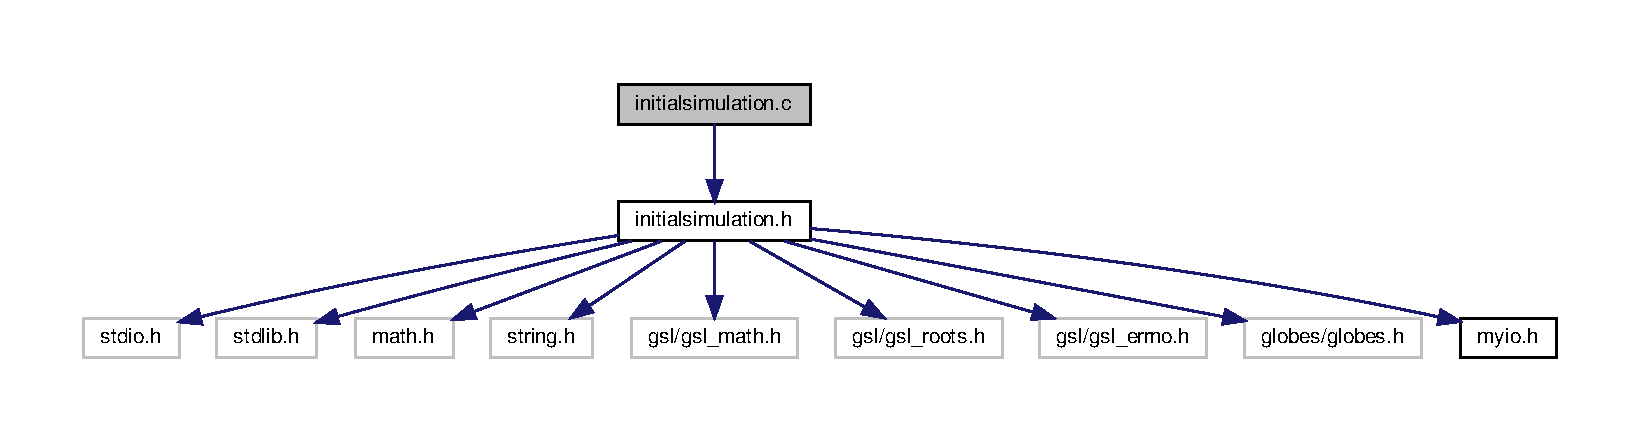
\includegraphics[width=350pt]{initialsimulation_8c__incl}
\end{center}
\end{figure}
\subsection*{Macros}
\begin{DoxyCompactItemize}
\item 
\#define \hyperlink{initialsimulation_8c_aa985f5d78fe22e2bf9115004a82d9008}{M\+A\+X\+\_\+\+S\+YS}~200
\item 
\#define \hyperlink{initialsimulation_8c_aff6f6215352e5d38380d9ce04a692c87}{E\+X\+P\+\_\+\+F\+AR}~0
\item 
\#define \hyperlink{initialsimulation_8c_ace970fbe7e3d2edb2ab0923fb12a9fc1}{E\+X\+P\+\_\+\+N\+E\+AR}~1
\end{DoxyCompactItemize}
\subsection*{Functions}
\begin{DoxyCompactItemize}
\item 
double \hyperlink{initialsimulation_8c_a2f8edc4561e9744ed4233b205fa7ec32}{min} (double x, double y)
\item 
double \hyperlink{initialsimulation_8c_a435ef393d7d5394df67d5da81c108c7d}{square} (double x)
\item 
double \hyperlink{initialsimulation_8c_ad87b3fdc467a8bb3d8b02bee4f76acac}{likelihood} (double true\+\_\+rate, double fit\+\_\+rate, double sqr\+\_\+sigma)
\item 
double \hyperlink{initialsimulation_8c_a526d68b687c952d000bac0c9d8fd4639}{chi\+D\+C\+Norm} (int exp, int rule, int n\+\_\+params, double $\ast$x, double $\ast$errors, void $\ast$user\+\_\+data)
\item 
double \hyperlink{initialsimulation_8c_aa3d32db5e12332300e78d8fc8de6184d}{chi\+D\+C\+Spectral} (int exp, int rule, int n\+\_\+params, double $\ast$x, double $\ast$errors, void $\ast$user\+\_\+data)
\item 
double \hyperlink{initialsimulation_8c_aa34890f04451218ee65fddd5810924e6}{Do\+Chi\+Square} (double x, void $\ast$dummy)
\item 
void \hyperlink{initialsimulation_8c_a98deac6879cfff61ffac7b16a3dcbdc4}{gsl\+Error} (const char $\ast$reason, const char $\ast$file, int line, int gsl\+\_\+errno)
\item 
void \hyperlink{initialsimulation_8c_a2acac04fd9fbdb6899edcf9aa40e7d0c}{Compute\+Sensitivity\+Curve} ()
\item 
int \hyperlink{initialsimulation_8c_a0ddf1224851353fc92bfbff6f499fa97}{main} (int argc, char $\ast$argv\mbox{[}$\,$\mbox{]})
\end{DoxyCompactItemize}
\subsection*{Variables}
\begin{DoxyCompactItemize}
\item 
char \hyperlink{initialsimulation_8c_a612d6b5b01674a0aec144bf224de6879}{M\+Y\+F\+I\+L\+E1} \mbox{[}$\,$\mbox{]} =\char`\"{}histsima.\+dat\char`\"{}
\item 
char \hyperlink{initialsimulation_8c_adfc2d3d253f6255b799065aa32d95cb2}{M\+Y\+F\+I\+L\+E2} \mbox{[}$\,$\mbox{]} =\char`\"{}histsimb.\+dat\char`\"{}
\item 
char \hyperlink{initialsimulation_8c_ac1dafa9fa032f3fd9126bad6b7a9850c}{M\+Y\+F\+I\+L\+E3} \mbox{[}$\,$\mbox{]} =\char`\"{}histsim1.\+dat\char`\"{}
\item 
double \hyperlink{initialsimulation_8c_a34595bc67066b681fdf55138851f5537}{theta12}
\item 
double \hyperlink{initialsimulation_8c_a16d90a56a2e53f1e0ce749a1924f5e91}{theta13}
\item 
double \hyperlink{initialsimulation_8c_ad7eb34b77c1ced121f217184784ca4ca}{theta23}
\item 
double \hyperlink{initialsimulation_8c_a9d56cc3e601b27fad6831203a4626bd2}{deltacp}
\item 
double \hyperlink{initialsimulation_8c_a188db76c6a2dc2aa72024eb9cfb5eee2}{sdm}
\item 
double \hyperlink{initialsimulation_8c_a3c9a8dabf1ad4dafa47e2d8002a71b44}{ldm}
\item 
glb\+\_\+params \hyperlink{initialsimulation_8c_a04b2e1a70c7d99ae440fc0b97b42bb2b}{true\+\_\+values}
\item 
glb\+\_\+params \hyperlink{initialsimulation_8c_a7b09cafa395dbf045d36fc6dad50319a}{test\+\_\+values}
\item 
glb\+\_\+params \hyperlink{initialsimulation_8c_a4849c92a9edd1a0b4d2ff01484cebc91}{input\+\_\+errors}
\item 
const gsl\+\_\+root\+\_\+fsolver\+\_\+type $\ast$ \hyperlink{initialsimulation_8c_a00bb11e935f05b5bb392ec7cc02a1478}{T}
\item 
gsl\+\_\+root\+\_\+fsolver $\ast$ \hyperlink{initialsimulation_8c_a9b42b07c83ecf6e931fc25d97a107cf0}{s}
\item 
gsl\+\_\+function \hyperlink{initialsimulation_8c_a76f2e70c9fc2a87ebcc598a0e021d2e6}{gsl\+\_\+func}
\item 
const double \hyperlink{initialsimulation_8c_a0a8e978504303b8dcd44cb9329b4cfc4}{min\+\_\+runtime} = 1e-\/2
\item 
const double \hyperlink{initialsimulation_8c_aa66d6bca132b398b255c2fd11ae6e7cc}{max\+\_\+runtime} = 1e4
\item 
const double \hyperlink{initialsimulation_8c_aa61745407a26c87961303a3c321dbba0}{chi2\+\_\+goal} = 2.\+7
\item 
const int \hyperlink{initialsimulation_8c_a8ceb9a82655d4344fa7db3b8d0dc8afb}{t\+Steps} = 30
\item 
const double \hyperlink{initialsimulation_8c_aa1edd4d864d9e90a1f10a7d13a68a885}{logs22th13\+\_\+precision} = 0.\+005
\item 
double \hyperlink{initialsimulation_8c_ac40fbcecee7fb042256f95763d5c1c68}{sys\+\_\+errors} \mbox{[}\hyperlink{initialsimulation_8c_aa985f5d78fe22e2bf9115004a82d9008}{M\+A\+X\+\_\+\+S\+YS}\mbox{]}
\item 
double \hyperlink{initialsimulation_8c_a6ce721d0fe57253b204857c23ed0e4db}{sys\+\_\+startval} \mbox{[}\hyperlink{initialsimulation_8c_aa985f5d78fe22e2bf9115004a82d9008}{M\+A\+X\+\_\+\+S\+YS}\mbox{]}
\item 
double \hyperlink{initialsimulation_8c_af986a51f33f1570fd3fc8186dd81d866}{sigma\+\_\+binbin} = 0.\+0
\end{DoxyCompactItemize}


\subsection{Macro Definition Documentation}
\mbox{\Hypertarget{initialsimulation_8c_aff6f6215352e5d38380d9ce04a692c87}\label{initialsimulation_8c_aff6f6215352e5d38380d9ce04a692c87}} 
\index{initialsimulation.\+c@{initialsimulation.\+c}!E\+X\+P\+\_\+\+F\+AR@{E\+X\+P\+\_\+\+F\+AR}}
\index{E\+X\+P\+\_\+\+F\+AR@{E\+X\+P\+\_\+\+F\+AR}!initialsimulation.\+c@{initialsimulation.\+c}}
\subsubsection{\texorpdfstring{E\+X\+P\+\_\+\+F\+AR}{EXP\_FAR}}
{\footnotesize\ttfamily \#define E\+X\+P\+\_\+\+F\+AR~0}



Definition at line 66 of file initialsimulation.\+c.



Referenced by chi\+D\+C\+Norm(), chi\+D\+C\+Spectral(), Compute\+Sensitivity\+Curve(), Do\+Chi\+Square(), and main().

\mbox{\Hypertarget{initialsimulation_8c_ace970fbe7e3d2edb2ab0923fb12a9fc1}\label{initialsimulation_8c_ace970fbe7e3d2edb2ab0923fb12a9fc1}} 
\index{initialsimulation.\+c@{initialsimulation.\+c}!E\+X\+P\+\_\+\+N\+E\+AR@{E\+X\+P\+\_\+\+N\+E\+AR}}
\index{E\+X\+P\+\_\+\+N\+E\+AR@{E\+X\+P\+\_\+\+N\+E\+AR}!initialsimulation.\+c@{initialsimulation.\+c}}
\subsubsection{\texorpdfstring{E\+X\+P\+\_\+\+N\+E\+AR}{EXP\_NEAR}}
{\footnotesize\ttfamily \#define E\+X\+P\+\_\+\+N\+E\+AR~1}



Definition at line 67 of file initialsimulation.\+c.



Referenced by chi\+D\+C\+Norm(), chi\+D\+C\+Spectral(), Compute\+Sensitivity\+Curve(), and main().

\mbox{\Hypertarget{initialsimulation_8c_aa985f5d78fe22e2bf9115004a82d9008}\label{initialsimulation_8c_aa985f5d78fe22e2bf9115004a82d9008}} 
\index{initialsimulation.\+c@{initialsimulation.\+c}!M\+A\+X\+\_\+\+S\+YS@{M\+A\+X\+\_\+\+S\+YS}}
\index{M\+A\+X\+\_\+\+S\+YS@{M\+A\+X\+\_\+\+S\+YS}!initialsimulation.\+c@{initialsimulation.\+c}}
\subsubsection{\texorpdfstring{M\+A\+X\+\_\+\+S\+YS}{MAX\_SYS}}
{\footnotesize\ttfamily \#define M\+A\+X\+\_\+\+S\+YS~200}



Definition at line 61 of file initialsimulation.\+c.



Referenced by main().



\subsection{Function Documentation}
\mbox{\Hypertarget{initialsimulation_8c_a526d68b687c952d000bac0c9d8fd4639}\label{initialsimulation_8c_a526d68b687c952d000bac0c9d8fd4639}} 
\index{initialsimulation.\+c@{initialsimulation.\+c}!chi\+D\+C\+Norm@{chi\+D\+C\+Norm}}
\index{chi\+D\+C\+Norm@{chi\+D\+C\+Norm}!initialsimulation.\+c@{initialsimulation.\+c}}
\subsubsection{\texorpdfstring{chi\+D\+C\+Norm()}{chiDCNorm()}}
{\footnotesize\ttfamily double chi\+D\+C\+Norm (\begin{DoxyParamCaption}\item[{int}]{exp,  }\item[{int}]{rule,  }\item[{int}]{n\+\_\+params,  }\item[{double $\ast$}]{x,  }\item[{double $\ast$}]{errors,  }\item[{void $\ast$}]{user\+\_\+data }\end{DoxyParamCaption})}



Definition at line 114 of file initialsimulation.\+c.



References E\+X\+P\+\_\+\+F\+AR, E\+X\+P\+\_\+\+N\+E\+AR, likelihood(), square(), and sys\+\_\+startval.



Referenced by main().


\begin{DoxyCode}
115                                  \{
116   \textcolor{keywordtype}{int} n\_bins = glbGetNumberOfBins(\hyperlink{initialsimulation_8c_aff6f6215352e5d38380d9ce04a692c87}{EXP\_FAR});
117   \textcolor{keywordtype}{double} *true\_rates\_N = glbGetRuleRatePtr(\hyperlink{initialsimulation_8c_ace970fbe7e3d2edb2ab0923fb12a9fc1}{EXP\_NEAR}, 0);
118   \textcolor{keywordtype}{double} *true\_rates\_F = glbGetRuleRatePtr(\hyperlink{initialsimulation_8c_aff6f6215352e5d38380d9ce04a692c87}{EXP\_FAR}, 0);
119   \textcolor{keywordtype}{double} signal\_fit\_rates\_N[n\_bins];
120   \textcolor{keywordtype}{double} signal\_fit\_rates\_F[n\_bins];
121   \textcolor{keywordtype}{double} signal\_norm\_N, signal\_norm\_F;
122   \textcolor{keywordtype}{int} ew\_low, ew\_high;
123   \textcolor{keywordtype}{double} emin, emax;
124   \textcolor{keywordtype}{double} fit\_rate;
125   \textcolor{keywordtype}{double} chi2 = 0.0;
126   \textcolor{keywordtype}{int} i;
127 
128   \textcolor{comment}{/* Request simulated energy interval and analysis energy window */}
129   glbGetEminEmax(exp, &emin, &emax);
130   glbGetEnergyWindowBins(exp, rule, &ew\_low, &ew\_high);
131 
132   \textcolor{comment}{/* Apply energy calibration error */}
133   glbShiftEnergyScale(\hyperlink{namespacequickplot_a81eab613e6132e2f34362e0d796374b6}{x}[3], glbGetSignalFitRatePtr(\hyperlink{initialsimulation_8c_aff6f6215352e5d38380d9ce04a692c87}{EXP\_FAR}, 0),
134                       signal\_fit\_rates\_F, n\_bins, emin, emax);
135   glbShiftEnergyScale(\hyperlink{namespacequickplot_a81eab613e6132e2f34362e0d796374b6}{x}[4], glbGetSignalFitRatePtr(\hyperlink{initialsimulation_8c_ace970fbe7e3d2edb2ab0923fb12a9fc1}{EXP\_NEAR}, 0),
136                       signal\_fit\_rates\_N, n\_bins, emin, emax);
137 
138   \textcolor{comment}{/* Loop over all bins in energy window */}
139   signal\_norm\_F = 1.0 + \hyperlink{namespacequickplot_a81eab613e6132e2f34362e0d796374b6}{x}[0] + \hyperlink{namespacequickplot_a81eab613e6132e2f34362e0d796374b6}{x}[1];
140   signal\_norm\_N = 1.0 + x[0] + x[2];
141   \textcolor{keywordflow}{for} (i=ew\_low; i <= ew\_high; i++)
142   \{
143     \textcolor{comment}{/* Statistical part of chi^2 for far detector}
144 \textcolor{comment}{     * Normalization is affected by flux error x[0] and fiducial mass error x[1] */}
145     fit\_rate  = signal\_norm\_F * signal\_fit\_rates\_F[i];
146     chi2 += \hyperlink{initialsimulation_8c_ad87b3fdc467a8bb3d8b02bee4f76acac}{likelihood}(true\_rates\_F[i], fit\_rate, true\_rates\_F[i]);
147 
148     \textcolor{comment}{/* Statistical part of chi^2 for near detector}
149 \textcolor{comment}{     * Normalization is affected by flux error x[0] and fiducial mass error x[2] */}
150     fit\_rate  = signal\_norm\_N * signal\_fit\_rates\_N[i];
151     chi2 += \hyperlink{initialsimulation_8c_ad87b3fdc467a8bb3d8b02bee4f76acac}{likelihood}(true\_rates\_N[i], fit\_rate, true\_rates\_N[i]);
152   \}
153 
154   \textcolor{comment}{/* Systematical part of chi^2 (= priors) */}
155   \textcolor{keywordflow}{for} (i=0; i < n\_params; i++)
156     chi2 += \hyperlink{initialsimulation_8c_a435ef393d7d5394df67d5da81c108c7d}{square}(x[i] / errors[i]);
157 
158   \textcolor{comment}{/* Save the systematics parameters as starting values for the next step */}
159   \textcolor{keywordflow}{for} (i=0; i < n\_params; i++)
160     \hyperlink{initialsimulation_8c_a6ce721d0fe57253b204857c23ed0e4db}{sys\_startval}[i] = x[i];
161 
162   \textcolor{keywordflow}{return} chi2;
163 \}
\end{DoxyCode}
Here is the call graph for this function\+:\nopagebreak
\begin{figure}[H]
\begin{center}
\leavevmode
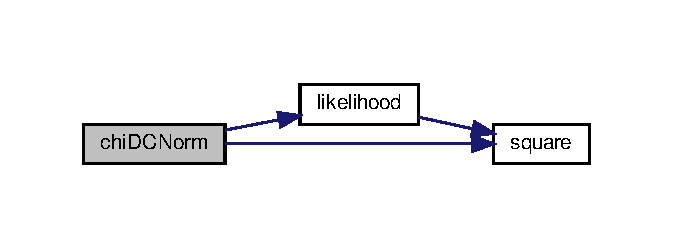
\includegraphics[width=323pt]{initialsimulation_8c_a526d68b687c952d000bac0c9d8fd4639_cgraph}
\end{center}
\end{figure}
Here is the caller graph for this function\+:\nopagebreak
\begin{figure}[H]
\begin{center}
\leavevmode
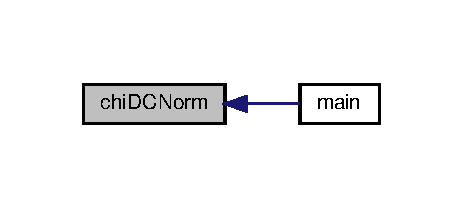
\includegraphics[width=222pt]{initialsimulation_8c_a526d68b687c952d000bac0c9d8fd4639_icgraph}
\end{center}
\end{figure}
\mbox{\Hypertarget{initialsimulation_8c_aa3d32db5e12332300e78d8fc8de6184d}\label{initialsimulation_8c_aa3d32db5e12332300e78d8fc8de6184d}} 
\index{initialsimulation.\+c@{initialsimulation.\+c}!chi\+D\+C\+Spectral@{chi\+D\+C\+Spectral}}
\index{chi\+D\+C\+Spectral@{chi\+D\+C\+Spectral}!initialsimulation.\+c@{initialsimulation.\+c}}
\subsubsection{\texorpdfstring{chi\+D\+C\+Spectral()}{chiDCSpectral()}}
{\footnotesize\ttfamily double chi\+D\+C\+Spectral (\begin{DoxyParamCaption}\item[{int}]{exp,  }\item[{int}]{rule,  }\item[{int}]{n\+\_\+params,  }\item[{double $\ast$}]{x,  }\item[{double $\ast$}]{errors,  }\item[{void $\ast$}]{user\+\_\+data }\end{DoxyParamCaption})}



Definition at line 178 of file initialsimulation.\+c.



References E\+X\+P\+\_\+\+F\+AR, E\+X\+P\+\_\+\+N\+E\+AR, likelihood(), sigma\+\_\+binbin, square(), and sys\+\_\+startval.



Referenced by main().


\begin{DoxyCode}
179                                      \{
180   \textcolor{keywordtype}{int} n\_bins = glbGetNumberOfBins(\hyperlink{initialsimulation_8c_aff6f6215352e5d38380d9ce04a692c87}{EXP\_FAR});
181   \textcolor{keywordtype}{double} *true\_rates\_N = glbGetRuleRatePtr(\hyperlink{initialsimulation_8c_ace970fbe7e3d2edb2ab0923fb12a9fc1}{EXP\_NEAR}, 0);
182   \textcolor{keywordtype}{double} *true\_rates\_F = glbGetRuleRatePtr(\hyperlink{initialsimulation_8c_aff6f6215352e5d38380d9ce04a692c87}{EXP\_FAR}, 0);
183   \textcolor{keywordtype}{double} signal\_fit\_rates\_N[n\_bins];
184   \textcolor{keywordtype}{double} signal\_fit\_rates\_F[n\_bins];
185   \textcolor{keywordtype}{double} signal\_norm\_N, signal\_norm\_F;
186   \textcolor{keywordtype}{int} ew\_low, ew\_high;
187   \textcolor{keywordtype}{double} emin, emax;
188   \textcolor{keywordtype}{double} fit\_rate;
189   \textcolor{keywordtype}{double} chi2 = 0.0;
190   \textcolor{keywordtype}{int} i;
191 
192   \textcolor{comment}{/* Request simulated energy interval and analysis energy window */}
193   glbGetEminEmax(exp, &emin, &emax);
194   glbGetEnergyWindowBins(exp, rule, &ew\_low, &ew\_high);
195 
196   \textcolor{comment}{/* Apply energy calibration error */}
197   glbShiftEnergyScale(\hyperlink{namespacequickplot_a81eab613e6132e2f34362e0d796374b6}{x}[3], glbGetSignalFitRatePtr(\hyperlink{initialsimulation_8c_aff6f6215352e5d38380d9ce04a692c87}{EXP\_FAR}, 0),
198                       signal\_fit\_rates\_F, n\_bins, emin, emax);
199   glbShiftEnergyScale(\hyperlink{namespacequickplot_a81eab613e6132e2f34362e0d796374b6}{x}[4], glbGetSignalFitRatePtr(\hyperlink{initialsimulation_8c_ace970fbe7e3d2edb2ab0923fb12a9fc1}{EXP\_NEAR}, 0),
200                       signal\_fit\_rates\_N, n\_bins, emin, emax);
201 
202   \textcolor{comment}{/* Loop over all bins in energy window */}
203   signal\_norm\_F = 1.0 + \hyperlink{namespacequickplot_a81eab613e6132e2f34362e0d796374b6}{x}[0] + \hyperlink{namespacequickplot_a81eab613e6132e2f34362e0d796374b6}{x}[1];
204   signal\_norm\_N = 1.0 + x[0] + x[2];
205   \textcolor{keywordflow}{for} (i=ew\_low; i <= ew\_high; i++)
206   \{
207     \textcolor{comment}{/* Statistical part of chi^2 for far detector}
208 \textcolor{comment}{     * Normalization is affected by flux error x[0], fiducial mass error x[1],}
209 \textcolor{comment}{     * spectral perturbations x[5+i], and bin-to-bin error sigma\_binbin */}
210     fit\_rate  = (signal\_norm\_F + x[5+i]) * signal\_fit\_rates\_F[i];
211     chi2 += \hyperlink{initialsimulation_8c_ad87b3fdc467a8bb3d8b02bee4f76acac}{likelihood}( true\_rates\_F[i], fit\_rate,
212                     true\_rates\_F[i] * (1.0 + true\_rates\_F[i]*\hyperlink{initialsimulation_8c_a435ef393d7d5394df67d5da81c108c7d}{square}(
      \hyperlink{initialsimulation_8c_af986a51f33f1570fd3fc8186dd81d866}{sigma\_binbin})) );
213 
214     \textcolor{comment}{/* Statistical part of chi^2 for near detector}
215 \textcolor{comment}{     * Normalization is affected by flux error x[0], fiducial mass error x[2],}
216 \textcolor{comment}{     * spectral perturbations x[5+i], and bin-to-bin error sigma\_binbin */}
217     fit\_rate  = (signal\_norm\_N + x[5+i]) * signal\_fit\_rates\_N[i];
218     chi2 += \hyperlink{initialsimulation_8c_ad87b3fdc467a8bb3d8b02bee4f76acac}{likelihood}( true\_rates\_N[i], fit\_rate,
219                     true\_rates\_N[i] * (1.0 + true\_rates\_N[i]*\hyperlink{initialsimulation_8c_a435ef393d7d5394df67d5da81c108c7d}{square}(
      \hyperlink{initialsimulation_8c_af986a51f33f1570fd3fc8186dd81d866}{sigma\_binbin})) );
220   \}
221 
222   \textcolor{comment}{/* Systematical part of chi^2 (= priors) */}
223   \textcolor{keywordflow}{for} (i=0; i < n\_params; i++)
224     chi2 += \hyperlink{initialsimulation_8c_a435ef393d7d5394df67d5da81c108c7d}{square}(x[i] / errors[i]);
225 
226   \textcolor{comment}{/* Save the systematics parameters as starting values for the next step */}
227   \textcolor{keywordflow}{for} (i=0; i < n\_params; i++)
228     \hyperlink{initialsimulation_8c_a6ce721d0fe57253b204857c23ed0e4db}{sys\_startval}[i] = x[i];
229 
230   \textcolor{keywordflow}{return} chi2;
231 \}
\end{DoxyCode}
Here is the call graph for this function\+:\nopagebreak
\begin{figure}[H]
\begin{center}
\leavevmode
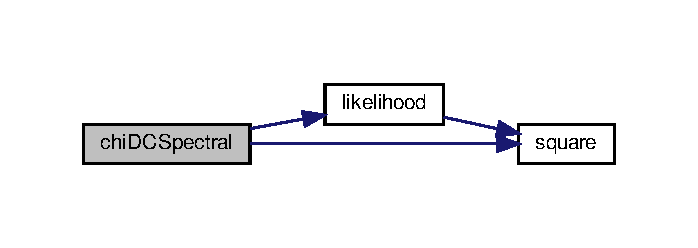
\includegraphics[width=335pt]{initialsimulation_8c_aa3d32db5e12332300e78d8fc8de6184d_cgraph}
\end{center}
\end{figure}
Here is the caller graph for this function\+:\nopagebreak
\begin{figure}[H]
\begin{center}
\leavevmode
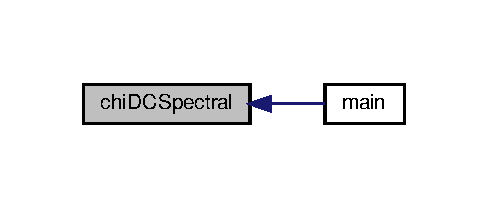
\includegraphics[width=234pt]{initialsimulation_8c_aa3d32db5e12332300e78d8fc8de6184d_icgraph}
\end{center}
\end{figure}
\mbox{\Hypertarget{initialsimulation_8c_a2acac04fd9fbdb6899edcf9aa40e7d0c}\label{initialsimulation_8c_a2acac04fd9fbdb6899edcf9aa40e7d0c}} 
\index{initialsimulation.\+c@{initialsimulation.\+c}!Compute\+Sensitivity\+Curve@{Compute\+Sensitivity\+Curve}}
\index{Compute\+Sensitivity\+Curve@{Compute\+Sensitivity\+Curve}!initialsimulation.\+c@{initialsimulation.\+c}}
\subsubsection{\texorpdfstring{Compute\+Sensitivity\+Curve()}{ComputeSensitivityCurve()}}
{\footnotesize\ttfamily void Compute\+Sensitivity\+Curve (\begin{DoxyParamCaption}{ }\end{DoxyParamCaption})}



Definition at line 274 of file initialsimulation.\+c.



References Add\+To\+Output2(), deltacp, E\+X\+P\+\_\+\+F\+AR, E\+X\+P\+\_\+\+N\+E\+AR, gsl\+\_\+func, input\+\_\+errors, ldm, logs22th13\+\_\+precision, max\+\_\+runtime, min(), min\+\_\+runtime, s, sdm, test\+\_\+values, theta12, theta13, theta23, true\+\_\+values, t\+Steps, and quickplot\+::x.



Referenced by main().


\begin{DoxyCode}
274                               \{
275   \textcolor{keywordtype}{double} t\_factor = pow(\hyperlink{initialsimulation_8c_aa66d6bca132b398b255c2fd11ae6e7cc}{max\_runtime}/\hyperlink{initialsimulation_8c_a0a8e978504303b8dcd44cb9329b4cfc4}{min\_runtime}, 1.0/
      \hyperlink{initialsimulation_8c_a8ceb9a82655d4344fa7db3b8d0dc8afb}{tSteps});
276   \textcolor{keywordtype}{double} t;
277   \textcolor{keywordtype}{double} \hyperlink{namespacequickplot_a81eab613e6132e2f34362e0d796374b6}{x};               \textcolor{comment}{/* Current value of log[sin^2(2*th13)] */}
278   \textcolor{keywordtype}{double} x\_lo, x\_hi;      \textcolor{comment}{/* Bracketing interval for root finder */}
279   \textcolor{keywordtype}{double} x\_sens[\hyperlink{initialsimulation_8c_a8ceb9a82655d4344fa7db3b8d0dc8afb}{tSteps}+1];\textcolor{comment}{/* Calculated sensitivities to log[sin^2(2*th13)] */}
280   \textcolor{keywordtype}{int} gsl\_status;         \textcolor{comment}{/* GSL error code */}
281   \textcolor{keywordtype}{int} iter;               \textcolor{comment}{/* Iteration counter for root finder */}
282   \textcolor{keyword}{const} \textcolor{keywordtype}{int} max\_iter=100; \textcolor{comment}{/* Maximum number of iterations allowed in root finder */}
283   \textcolor{keywordtype}{int} j;
284 
285   \textcolor{keywordflow}{for} (j=0; j <= \hyperlink{initialsimulation_8c_a8ceb9a82655d4344fa7db3b8d0dc8afb}{tSteps}; j++)      \textcolor{comment}{/* Initialize output vector */}
286     x\_sens[j] = 1;                 \textcolor{comment}{/* As x is always <= 0 this signals "no value" */}
287 
288   \textcolor{comment}{/* Loop over all data points in this dataset, using log stepping */}
289   \textcolor{keywordflow}{for} (j=0; j <= \hyperlink{initialsimulation_8c_a8ceb9a82655d4344fa7db3b8d0dc8afb}{tSteps}; j++)
290   \{
291     \textcolor{comment}{/* Set running time */}
292     t = \hyperlink{initialsimulation_8c_a0a8e978504303b8dcd44cb9329b4cfc4}{min\_runtime} * pow(t\_factor,j);
293     glbSetRunningTime(\hyperlink{initialsimulation_8c_aff6f6215352e5d38380d9ce04a692c87}{EXP\_FAR}, 0, t);
294     glbSetRunningTime(\hyperlink{initialsimulation_8c_ace970fbe7e3d2edb2ab0923fb12a9fc1}{EXP\_NEAR}, 0, t);
295 
296     \textcolor{comment}{/* Calculate "true" event rates */}
297     glbDefineParams(\hyperlink{initialsimulation_8c_a04b2e1a70c7d99ae440fc0b97b42bb2b}{true\_values},\hyperlink{initialsimulation_8c_a34595bc67066b681fdf55138851f5537}{theta12},\hyperlink{initialsimulation_8c_a16d90a56a2e53f1e0ce749a1924f5e91}{theta13},\hyperlink{initialsimulation_8c_ad7eb34b77c1ced121f217184784ca4ca}{theta23},
      \hyperlink{initialsimulation_8c_a9d56cc3e601b27fad6831203a4626bd2}{deltacp},\hyperlink{initialsimulation_8c_a188db76c6a2dc2aa72024eb9cfb5eee2}{sdm},\hyperlink{initialsimulation_8c_a3c9a8dabf1ad4dafa47e2d8002a71b44}{ldm});
298     glbSetDensityParams(\hyperlink{initialsimulation_8c_a04b2e1a70c7d99ae440fc0b97b42bb2b}{true\_values},1.0,GLB\_ALL);
299     glbDefineParams(\hyperlink{initialsimulation_8c_a7b09cafa395dbf045d36fc6dad50319a}{test\_values},\hyperlink{initialsimulation_8c_a34595bc67066b681fdf55138851f5537}{theta12},\hyperlink{initialsimulation_8c_a16d90a56a2e53f1e0ce749a1924f5e91}{theta13},\hyperlink{initialsimulation_8c_ad7eb34b77c1ced121f217184784ca4ca}{theta23},
      \hyperlink{initialsimulation_8c_a9d56cc3e601b27fad6831203a4626bd2}{deltacp},\hyperlink{initialsimulation_8c_a188db76c6a2dc2aa72024eb9cfb5eee2}{sdm},\hyperlink{initialsimulation_8c_a3c9a8dabf1ad4dafa47e2d8002a71b44}{ldm});
300     glbSetDensityParams(\hyperlink{initialsimulation_8c_a7b09cafa395dbf045d36fc6dad50319a}{test\_values},1.0,GLB\_ALL);
301     glbDefineParams(\hyperlink{initialsimulation_8c_a4849c92a9edd1a0b4d2ff01484cebc91}{input\_errors}, 0.1*\hyperlink{initialsimulation_8c_a34595bc67066b681fdf55138851f5537}{theta12}, 0, 0.15*
      \hyperlink{initialsimulation_8c_ad7eb34b77c1ced121f217184784ca4ca}{theta23}, 0, 0.05*\hyperlink{initialsimulation_8c_a188db76c6a2dc2aa72024eb9cfb5eee2}{sdm}, 0.05*\hyperlink{initialsimulation_8c_a3c9a8dabf1ad4dafa47e2d8002a71b44}{ldm});
302     glbSetDensityParams(\hyperlink{initialsimulation_8c_a4849c92a9edd1a0b4d2ff01484cebc91}{input\_errors}, 0.05, GLB\_ALL);
303     glbSetOscillationParameters(\hyperlink{initialsimulation_8c_a04b2e1a70c7d99ae440fc0b97b42bb2b}{true\_values});
304     glbSetInputErrors(\hyperlink{initialsimulation_8c_a4849c92a9edd1a0b4d2ff01484cebc91}{input\_errors});
305     glbSetRates();
306 
307     \textcolor{comment}{/* Determine sensitivity to sin^2(2*th13) by  using the GSL Brent-Dekker}
308 \textcolor{comment}{     * algorithm to find the th13, for which chi^2 = 2.7 (90%) */}
309     x\_lo = -3.0;
310     x\_hi = -0.1;
311     iter = 0;
312 
313     \textcolor{comment}{/* Start root finder. The initial search interval is guessed based on the}
314 \textcolor{comment}{     * results from a neighboring grid point */}
315     \textcolor{keywordtype}{double} deviation=0.1;
316     \textcolor{keywordflow}{do} \{
317       \textcolor{keywordflow}{if} (j > 0) \{
318         x\_lo = x\_sens[j-1] - deviation;
319         x\_hi = \hyperlink{initialsimulation_8c_a2f8edc4561e9744ed4233b205fa7ec32}{min}(x\_sens[j-1] + deviation, -0.001);
320       \}
321       gsl\_status = gsl\_root\_fsolver\_set(\hyperlink{initialsimulation_8c_a9b42b07c83ecf6e931fc25d97a107cf0}{s}, &\hyperlink{initialsimulation_8c_a76f2e70c9fc2a87ebcc598a0e021d2e6}{gsl\_func}, x\_lo, x\_hi);
322       deviation *= 2;
323     \} \textcolor{keywordflow}{while} (gsl\_status != GSL\_SUCCESS);
324 
325     \textcolor{comment}{/* Iterate root finder */}
326     \textcolor{keywordflow}{do} \{
327       gsl\_status = gsl\_root\_fsolver\_iterate(\hyperlink{initialsimulation_8c_a9b42b07c83ecf6e931fc25d97a107cf0}{s});
328       x          = gsl\_root\_fsolver\_root(\hyperlink{initialsimulation_8c_a9b42b07c83ecf6e931fc25d97a107cf0}{s});
329       x\_lo       = gsl\_root\_fsolver\_x\_lower(\hyperlink{initialsimulation_8c_a9b42b07c83ecf6e931fc25d97a107cf0}{s});
330       x\_hi       = gsl\_root\_fsolver\_x\_upper(\hyperlink{initialsimulation_8c_a9b42b07c83ecf6e931fc25d97a107cf0}{s});
331       gsl\_status = gsl\_root\_test\_interval (x\_lo, x\_hi, \hyperlink{initialsimulation_8c_aa1edd4d864d9e90a1f10a7d13a68a885}{logs22th13\_precision}, 0);
332     \} \textcolor{keywordflow}{while} (gsl\_status == GSL\_CONTINUE && iter < max\_iter);
333 
334     \textcolor{comment}{/* Save results */}
335     x\_sens[j] = \hyperlink{namespacequickplot_a81eab613e6132e2f34362e0d796374b6}{x};
336     \hyperlink{myio_8c_ae9af054c63cf3b736da1ee7151f69d2c}{AddToOutput2}(t, x);
337 
339 
340   \textcolor{comment}{// Setting up output}
341 
342   \textcolor{keywordtype}{int} max\_channel\_id = 17;
343 
344   \textcolor{keywordtype}{char} buf[60];
345   \textcolor{keywordtype}{char} str[60];
346 
347   \textcolor{keywordflow}{for}(\textcolor{keywordtype}{int} i=0; i<max\_channel\_id+1;i++)\{
348 
349     sprintf(buf,\textcolor{stringliteral}{"%dtime2histsim\_channel%d.dat"},j,i);
350     strcpy(str,buf);
351 
352     FILE* f\_out = fopen(str,\textcolor{stringliteral}{"w"});
353 
354     
355     \textcolor{comment}{// double hist\_time = 100000;}
356     \textcolor{comment}{// glbSetRunningTime(EXP\_NEAR,0,hist\_time);}
357 
358     \textcolor{comment}{//printf("Running time is; %f",glbGetRunningTime(1,0));}
359 
360     glbShowChannelRates(f\_out,\hyperlink{initialsimulation_8c_ace970fbe7e3d2edb2ab0923fb12a9fc1}{EXP\_NEAR},i,GLB\_PRE,GLB\_WO\_EFF,GLB\_WO\_BG);
361 
362   fclose(f\_out);
363 
364 
365   \}
366 
367   \}
368 \}
\end{DoxyCode}
Here is the call graph for this function\+:
\nopagebreak
\begin{figure}[H]
\begin{center}
\leavevmode
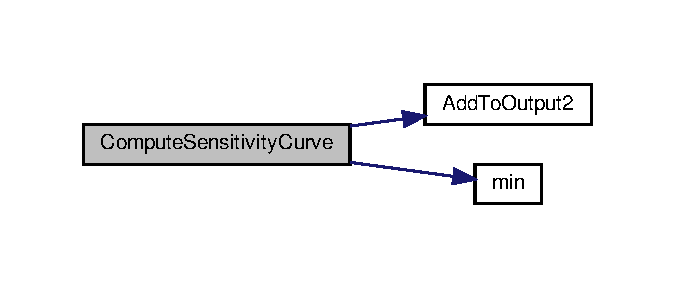
\includegraphics[width=324pt]{initialsimulation_8c_a2acac04fd9fbdb6899edcf9aa40e7d0c_cgraph}
\end{center}
\end{figure}
Here is the caller graph for this function\+:\nopagebreak
\begin{figure}[H]
\begin{center}
\leavevmode
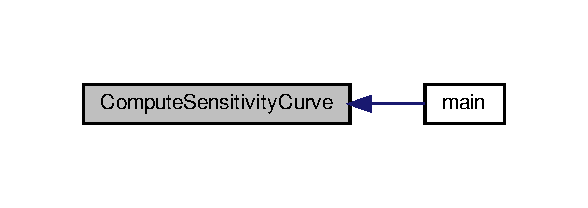
\includegraphics[width=282pt]{initialsimulation_8c_a2acac04fd9fbdb6899edcf9aa40e7d0c_icgraph}
\end{center}
\end{figure}
\mbox{\Hypertarget{initialsimulation_8c_aa34890f04451218ee65fddd5810924e6}\label{initialsimulation_8c_aa34890f04451218ee65fddd5810924e6}} 
\index{initialsimulation.\+c@{initialsimulation.\+c}!Do\+Chi\+Square@{Do\+Chi\+Square}}
\index{Do\+Chi\+Square@{Do\+Chi\+Square}!initialsimulation.\+c@{initialsimulation.\+c}}
\subsubsection{\texorpdfstring{Do\+Chi\+Square()}{DoChiSquare()}}
{\footnotesize\ttfamily double Do\+Chi\+Square (\begin{DoxyParamCaption}\item[{double}]{x,  }\item[{void $\ast$}]{dummy }\end{DoxyParamCaption})}



Definition at line 239 of file initialsimulation.\+c.



References chi2\+\_\+goal, E\+X\+P\+\_\+\+F\+AR, sys\+\_\+startval, and test\+\_\+values.



Referenced by main().


\begin{DoxyCode}
239                                          \{
240   \textcolor{keywordtype}{double} thetheta13, chi2;
241 
242   \textcolor{comment}{/* Set vector of test values */}
243   thetheta13 = asin(sqrt(pow(10,\hyperlink{namespacequickplot_a81eab613e6132e2f34362e0d796374b6}{x})))/2;
244   glbSetOscParams(\hyperlink{initialsimulation_8c_a7b09cafa395dbf045d36fc6dad50319a}{test\_values}, thetheta13, GLB\_THETA\_13);
245   glbSetOscParams(\hyperlink{initialsimulation_8c_a7b09cafa395dbf045d36fc6dad50319a}{test\_values}, 200.0/2 * (\hyperlink{namespacequickplot_a81eab613e6132e2f34362e0d796374b6}{x}+4)*M\_PI/180, GLB\_DELTA\_CP);
246 
247   \textcolor{comment}{/* Set starting values for systematics minimiyer to the coordinates of}
248 \textcolor{comment}{   * minimum in the last iteration. This accelerates the minimization and}
249 \textcolor{comment}{   * prevents convergence problems. */}
250   glbSetSysStartingValuesList(\hyperlink{initialsimulation_8c_aff6f6215352e5d38380d9ce04a692c87}{EXP\_FAR}, 0, GLB\_ON, \hyperlink{initialsimulation_8c_a6ce721d0fe57253b204857c23ed0e4db}{sys\_startval});
251 
252   \textcolor{comment}{/* Compute Chi^2 for all loaded experiments and all rules}
253 \textcolor{comment}{   * Correlations are unimportant in reactor experiments, so glbChiSys is sufficient */}
254   chi2 = glbChiSys(\hyperlink{initialsimulation_8c_a7b09cafa395dbf045d36fc6dad50319a}{test\_values}, GLB\_ALL, GLB\_ALL);
255 
256   \textcolor{keywordflow}{return} chi2 - \hyperlink{initialsimulation_8c_aa61745407a26c87961303a3c321dbba0}{chi2\_goal};
257 \}
\end{DoxyCode}
Here is the caller graph for this function\+:\nopagebreak
\begin{figure}[H]
\begin{center}
\leavevmode
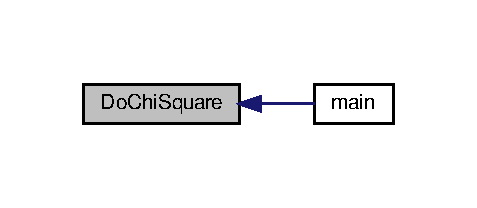
\includegraphics[width=229pt]{initialsimulation_8c_aa34890f04451218ee65fddd5810924e6_icgraph}
\end{center}
\end{figure}
\mbox{\Hypertarget{initialsimulation_8c_a98deac6879cfff61ffac7b16a3dcbdc4}\label{initialsimulation_8c_a98deac6879cfff61ffac7b16a3dcbdc4}} 
\index{initialsimulation.\+c@{initialsimulation.\+c}!gsl\+Error@{gsl\+Error}}
\index{gsl\+Error@{gsl\+Error}!initialsimulation.\+c@{initialsimulation.\+c}}
\subsubsection{\texorpdfstring{gsl\+Error()}{gslError()}}
{\footnotesize\ttfamily void gsl\+Error (\begin{DoxyParamCaption}\item[{const char $\ast$}]{reason,  }\item[{const char $\ast$}]{file,  }\item[{int}]{line,  }\item[{int}]{gsl\+\_\+errno }\end{DoxyParamCaption})}



Definition at line 261 of file initialsimulation.\+c.



Referenced by main().


\begin{DoxyCode}
261                                                                             \{
262   \textcolor{keyword}{static} \textcolor{keywordtype}{int} n\_errors=0;
263 
264   printf(\textcolor{stringliteral}{"GSL Error in file %s:%d : %s\(\backslash\)n"}, file, line, gsl\_strerror(gsl\_errno));
265   \textcolor{keywordflow}{if} (++n\_errors > 1000)
266   \{
267     printf(\textcolor{stringliteral}{"Too many GSL errors. Program aborted.\(\backslash\)n"});
268     abort();
269   \}
270 \}
\end{DoxyCode}
Here is the caller graph for this function\+:\nopagebreak
\begin{figure}[H]
\begin{center}
\leavevmode
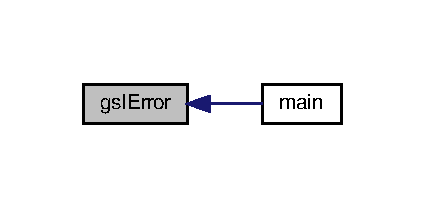
\includegraphics[width=204pt]{initialsimulation_8c_a98deac6879cfff61ffac7b16a3dcbdc4_icgraph}
\end{center}
\end{figure}
\mbox{\Hypertarget{initialsimulation_8c_ad87b3fdc467a8bb3d8b02bee4f76acac}\label{initialsimulation_8c_ad87b3fdc467a8bb3d8b02bee4f76acac}} 
\index{initialsimulation.\+c@{initialsimulation.\+c}!likelihood@{likelihood}}
\index{likelihood@{likelihood}!initialsimulation.\+c@{initialsimulation.\+c}}
\subsubsection{\texorpdfstring{likelihood()}{likelihood()}}
{\footnotesize\ttfamily double likelihood (\begin{DoxyParamCaption}\item[{double}]{true\+\_\+rate,  }\item[{double}]{fit\+\_\+rate,  }\item[{double}]{sqr\+\_\+sigma }\end{DoxyParamCaption})\hspace{0.3cm}{\ttfamily [inline]}}



Definition at line 91 of file initialsimulation.\+c.



References square().



Referenced by chi\+D\+C\+Norm(), and chi\+D\+C\+Spectral().


\begin{DoxyCode}
92 \{
93   \textcolor{keywordflow}{if} (sqr\_sigma > 0)
94     \textcolor{keywordflow}{return} \hyperlink{initialsimulation_8c_a435ef393d7d5394df67d5da81c108c7d}{square}(true\_rate - fit\_rate) / sqr\_sigma;
95   \textcolor{keywordflow}{else}
96     \textcolor{keywordflow}{return} 0.0;
97 \}
\end{DoxyCode}
Here is the call graph for this function\+:\nopagebreak
\begin{figure}[H]
\begin{center}
\leavevmode
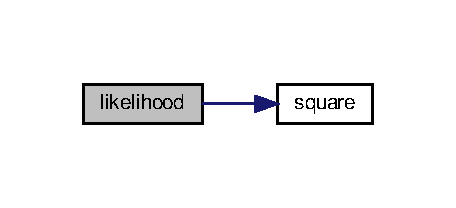
\includegraphics[width=219pt]{initialsimulation_8c_ad87b3fdc467a8bb3d8b02bee4f76acac_cgraph}
\end{center}
\end{figure}
Here is the caller graph for this function\+:\nopagebreak
\begin{figure}[H]
\begin{center}
\leavevmode
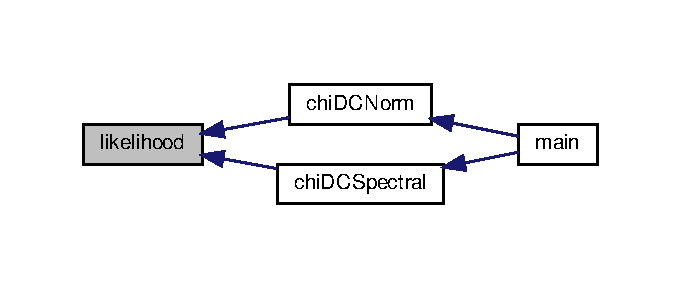
\includegraphics[width=327pt]{initialsimulation_8c_ad87b3fdc467a8bb3d8b02bee4f76acac_icgraph}
\end{center}
\end{figure}
\mbox{\Hypertarget{initialsimulation_8c_a0ddf1224851353fc92bfbff6f499fa97}\label{initialsimulation_8c_a0ddf1224851353fc92bfbff6f499fa97}} 
\index{initialsimulation.\+c@{initialsimulation.\+c}!main@{main}}
\index{main@{main}!initialsimulation.\+c@{initialsimulation.\+c}}
\subsubsection{\texorpdfstring{main()}{main()}}
{\footnotesize\ttfamily int main (\begin{DoxyParamCaption}\item[{int}]{argc,  }\item[{char $\ast$}]{argv\mbox{[}$\,$\mbox{]} }\end{DoxyParamCaption})}



Definition at line 375 of file initialsimulation.\+c.



References chi\+D\+C\+Norm(), chi\+D\+C\+Spectral(), Compute\+Sensitivity\+Curve(), deltacp, Do\+Chi\+Square(), E\+X\+P\+\_\+\+F\+AR, E\+X\+P\+\_\+\+N\+E\+AR, gsl\+\_\+func, gsl\+Error(), Init\+Output(), input\+\_\+errors, ldm, M\+A\+X\+\_\+\+S\+YS, M\+Y\+F\+I\+L\+E1, M\+Y\+F\+I\+L\+E2, s, sdm, sys\+\_\+startval, T, test\+\_\+values, theta12, theta13, theta23, and true\+\_\+values.


\begin{DoxyCode}
376 \{
377   \textcolor{keywordtype}{double} *old\_sys\_errors = NULL;      \textcolor{comment}{/* Temp. pointer to systematical error array */}
378   \textcolor{keywordtype}{int} sys\_dim;                        \textcolor{comment}{/* Abbrv. for number of systematical errors */}
379   \textcolor{keywordtype}{int} n\_bins=86;                      \textcolor{comment}{/* Number of bins */}
380   \textcolor{keywordtype}{int} i;
381 
382   \textcolor{comment}{/* Initialization */}
383   \textcolor{keywordflow}{for} (i=0; i < \hyperlink{initialsimulation_8c_aa985f5d78fe22e2bf9115004a82d9008}{MAX\_SYS}; i++)
384     \hyperlink{initialsimulation_8c_a6ce721d0fe57253b204857c23ed0e4db}{sys\_startval}[i] = 0.0;
385 
386   \textcolor{comment}{/* Set standard oscillation parameters (cf. hep-ph/0405172v5) */}
387   \hyperlink{initialsimulation_8c_a34595bc67066b681fdf55138851f5537}{theta12} = asin(sqrt(0.3));
388   \hyperlink{initialsimulation_8c_a16d90a56a2e53f1e0ce749a1924f5e91}{theta13} = 0.0;
389   \hyperlink{initialsimulation_8c_ad7eb34b77c1ced121f217184784ca4ca}{theta23} = M\_PI/4;
390   \hyperlink{initialsimulation_8c_a9d56cc3e601b27fad6831203a4626bd2}{deltacp} = M\_PI/2;
391   \hyperlink{initialsimulation_8c_a188db76c6a2dc2aa72024eb9cfb5eee2}{sdm} = 7.9e-5;
392   \hyperlink{initialsimulation_8c_a3c9a8dabf1ad4dafa47e2d8002a71b44}{ldm} = 2.6e-3;
393 
394   glbInit(argv[0]);                    \textcolor{comment}{/* Initialize GLoBES and define chi^2 functions */}
395   glbDefineChiFunction(&\hyperlink{initialsimulation_8c_a526d68b687c952d000bac0c9d8fd4639}{chiDCNorm},     5,        \textcolor{stringliteral}{"chiDCNorm"},     NULL);
396   glbDefineChiFunction(&\hyperlink{initialsimulation_8c_aa3d32db5e12332300e78d8fc8de6184d}{chiDCSpectral}, 5+n\_bins, \textcolor{stringliteral}{"chiDCSpectral"}, NULL);
397 
398   gsl\_set\_error\_handler(&\hyperlink{initialsimulation_8c_a98deac6879cfff61ffac7b16a3dcbdc4}{gslError});    \textcolor{comment}{/* Initialize GSL root finder */}
399   \hyperlink{initialsimulation_8c_a76f2e70c9fc2a87ebcc598a0e021d2e6}{gsl\_func}.function = &\hyperlink{initialsimulation_8c_aa34890f04451218ee65fddd5810924e6}{DoChiSquare};
400   \hyperlink{initialsimulation_8c_a76f2e70c9fc2a87ebcc598a0e021d2e6}{gsl\_func}.params   = NULL;
401   \hyperlink{initialsimulation_8c_a00bb11e935f05b5bb392ec7cc02a1478}{T} = gsl\_root\_fsolver\_brent;
402   \hyperlink{initialsimulation_8c_a9b42b07c83ecf6e931fc25d97a107cf0}{s} = gsl\_root\_fsolver\_alloc(\hyperlink{initialsimulation_8c_a00bb11e935f05b5bb392ec7cc02a1478}{T});
403 
404   \textcolor{comment}{/* Load 2 experiments: DC far (#0) and near (#1) detectors */}
405   glbClearExperimentList();
406   glbInitExperiment(\textcolor{stringliteral}{"CHIPS-GLB/glb-CHIPS10-7mrad-ME-FAR.glb"}, &glb\_experiment\_list[0], &glb\_num\_of\_exps);
407   glbInitExperiment(\textcolor{stringliteral}{"CHIPS-GLB/glb-CHIPS10-7mrad-ME-NEAR.glb"}, &glb\_experiment\_list[0], &glb\_num\_of\_exps);
408   \textcolor{keywordflow}{if} (glbGetNumberOfBins(\hyperlink{initialsimulation_8c_aff6f6215352e5d38380d9ce04a692c87}{EXP\_FAR}) != n\_bins || glbGetNumberOfBins(
      \hyperlink{initialsimulation_8c_ace970fbe7e3d2edb2ab0923fb12a9fc1}{EXP\_NEAR}) != n\_bins)
409   \{
410     printf(\textcolor{stringliteral}{"ERROR: Number of bins changed in AEDL file, but not in C code (or vice-versa).\(\backslash\)n"});
411     printf(\textcolor{stringliteral}{"nbins %i"},n\_bins);
412     printf(\textcolor{stringliteral}{"far bins %i"},glbGetNumberOfBins(\hyperlink{initialsimulation_8c_aff6f6215352e5d38380d9ce04a692c87}{EXP\_FAR}));
413     printf(\textcolor{stringliteral}{"near bins %i"},glbGetNumberOfBins(\hyperlink{initialsimulation_8c_ace970fbe7e3d2edb2ab0923fb12a9fc1}{EXP\_NEAR}));
414 
415     \textcolor{keywordflow}{return} -1;
416   \}
417   \textcolor{keywordflow}{else}
418     n\_bins = glbGetNumberOfBins(\hyperlink{initialsimulation_8c_aff6f6215352e5d38380d9ce04a692c87}{EXP\_FAR});
419 
420   \textcolor{comment}{/* Initialize parameter vectors */}
421   \hyperlink{initialsimulation_8c_a04b2e1a70c7d99ae440fc0b97b42bb2b}{true\_values}  = glbAllocParams();
422   \hyperlink{initialsimulation_8c_a7b09cafa395dbf045d36fc6dad50319a}{test\_values}  = glbAllocParams();
423   \hyperlink{initialsimulation_8c_a4849c92a9edd1a0b4d2ff01484cebc91}{input\_errors} = glbAllocParams();
424   glbDefineParams(\hyperlink{initialsimulation_8c_a04b2e1a70c7d99ae440fc0b97b42bb2b}{true\_values},\hyperlink{initialsimulation_8c_a34595bc67066b681fdf55138851f5537}{theta12},\hyperlink{initialsimulation_8c_a16d90a56a2e53f1e0ce749a1924f5e91}{theta13},\hyperlink{initialsimulation_8c_ad7eb34b77c1ced121f217184784ca4ca}{theta23},
      \hyperlink{initialsimulation_8c_a9d56cc3e601b27fad6831203a4626bd2}{deltacp},\hyperlink{initialsimulation_8c_a188db76c6a2dc2aa72024eb9cfb5eee2}{sdm},\hyperlink{initialsimulation_8c_a3c9a8dabf1ad4dafa47e2d8002a71b44}{ldm});
425   glbSetDensityParams(\hyperlink{initialsimulation_8c_a04b2e1a70c7d99ae440fc0b97b42bb2b}{true\_values},1.0,GLB\_ALL);
426   glbDefineParams(\hyperlink{initialsimulation_8c_a7b09cafa395dbf045d36fc6dad50319a}{test\_values},\hyperlink{initialsimulation_8c_a34595bc67066b681fdf55138851f5537}{theta12},\hyperlink{initialsimulation_8c_a16d90a56a2e53f1e0ce749a1924f5e91}{theta13},\hyperlink{initialsimulation_8c_ad7eb34b77c1ced121f217184784ca4ca}{theta23},
      \hyperlink{initialsimulation_8c_a9d56cc3e601b27fad6831203a4626bd2}{deltacp},\hyperlink{initialsimulation_8c_a188db76c6a2dc2aa72024eb9cfb5eee2}{sdm},\hyperlink{initialsimulation_8c_a3c9a8dabf1ad4dafa47e2d8002a71b44}{ldm});
427   glbSetDensityParams(\hyperlink{initialsimulation_8c_a7b09cafa395dbf045d36fc6dad50319a}{test\_values},1.0,GLB\_ALL);
428   glbDefineParams(\hyperlink{initialsimulation_8c_a4849c92a9edd1a0b4d2ff01484cebc91}{input\_errors}, 0.1*\hyperlink{initialsimulation_8c_a34595bc67066b681fdf55138851f5537}{theta12}, 0, 0.15*\hyperlink{initialsimulation_8c_ad7eb34b77c1ced121f217184784ca4ca}{theta23}, 0, 0.05*
      \hyperlink{initialsimulation_8c_a188db76c6a2dc2aa72024eb9cfb5eee2}{sdm}, 0.05*\hyperlink{initialsimulation_8c_a3c9a8dabf1ad4dafa47e2d8002a71b44}{ldm});
429   glbSetDensityParams(\hyperlink{initialsimulation_8c_a4849c92a9edd1a0b4d2ff01484cebc91}{input\_errors}, 0.05, GLB\_ALL);
430   glbSetOscillationParameters(\hyperlink{initialsimulation_8c_a04b2e1a70c7d99ae440fc0b97b42bb2b}{true\_values});
431   glbSetInputErrors(\hyperlink{initialsimulation_8c_a4849c92a9edd1a0b4d2ff01484cebc91}{input\_errors});
432 
433   \textcolor{comment}{/* Calculate sensitivity curve without systematics */}
434   \hyperlink{myio_8c_ad28713ee02cd79dc48ad1ee2a7b62177}{InitOutput}(\hyperlink{initialsimulation_8c_a612d6b5b01674a0aec144bf224de6879}{MYFILE1},\textcolor{stringliteral}{"Format: Running time   Log(10,s22th13) sens. \(\backslash\)n"});
435   glbSwitchSystematics(GLB\_ALL, GLB\_ALL, GLB\_OFF);
436   \hyperlink{initialsimulation_8c_a2acac04fd9fbdb6899edcf9aa40e7d0c}{ComputeSensitivityCurve}();
437   glbSwitchSystematics(GLB\_ALL, GLB\_ALL, GLB\_ON);
438 
439   \textcolor{comment}{/* Calculate sensitivity curve with normalization and energy calibration errors,}
440 \textcolor{comment}{   * as defined in the AEDL files */}
441   \hyperlink{myio_8c_ad28713ee02cd79dc48ad1ee2a7b62177}{InitOutput}(\hyperlink{initialsimulation_8c_adfc2d3d253f6255b799065aa32d95cb2}{MYFILE2},\textcolor{stringliteral}{"Format: Running time   Log(10,s22th13) sens. \(\backslash\)n"});
442   \hyperlink{initialsimulation_8c_a2acac04fd9fbdb6899edcf9aa40e7d0c}{ComputeSensitivityCurve}();
443 
444   printf(\textcolor{stringliteral}{"Number of channels: %d"},glbGetNumberOfChannels(\hyperlink{initialsimulation_8c_ace970fbe7e3d2edb2ab0923fb12a9fc1}{EXP\_NEAR}));
445 
446   \textcolor{keywordflow}{for}(\textcolor{keywordtype}{int} js = 0; js<=18;js++)\{
447   printf(\textcolor{stringliteral}{"Channel: %s"},glbValueToName(\hyperlink{initialsimulation_8c_ace970fbe7e3d2edb2ab0923fb12a9fc1}{EXP\_NEAR},\textcolor{stringliteral}{"channel"},js));
448   \}  
449   
450 
451   \textcolor{comment}{/* Clean up */}
452   glbFreeParams(\hyperlink{initialsimulation_8c_a04b2e1a70c7d99ae440fc0b97b42bb2b}{true\_values});
453   glbFreeParams(\hyperlink{initialsimulation_8c_a7b09cafa395dbf045d36fc6dad50319a}{test\_values});
454   glbFreeParams(\hyperlink{initialsimulation_8c_a4849c92a9edd1a0b4d2ff01484cebc91}{input\_errors});
455   gsl\_root\_fsolver\_free(\hyperlink{initialsimulation_8c_a9b42b07c83ecf6e931fc25d97a107cf0}{s});
456 
457   \textcolor{keywordflow}{return} 0;
458 \}
\end{DoxyCode}
Here is the call graph for this function\+:
\nopagebreak
\begin{figure}[H]
\begin{center}
\leavevmode
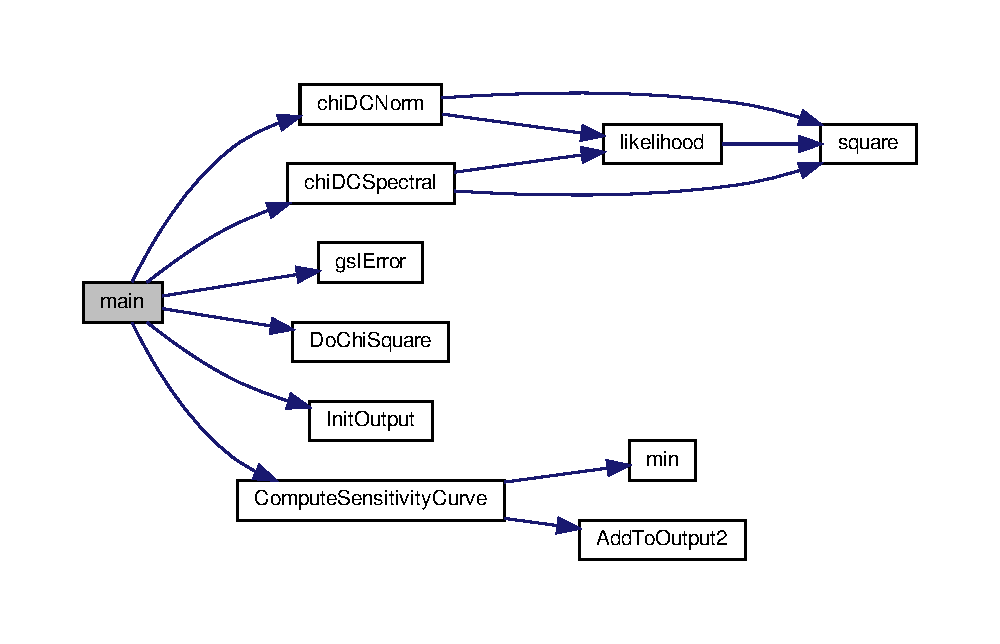
\includegraphics[width=350pt]{initialsimulation_8c_a0ddf1224851353fc92bfbff6f499fa97_cgraph}
\end{center}
\end{figure}
\mbox{\Hypertarget{initialsimulation_8c_a2f8edc4561e9744ed4233b205fa7ec32}\label{initialsimulation_8c_a2f8edc4561e9744ed4233b205fa7ec32}} 
\index{initialsimulation.\+c@{initialsimulation.\+c}!min@{min}}
\index{min@{min}!initialsimulation.\+c@{initialsimulation.\+c}}
\subsubsection{\texorpdfstring{min()}{min()}}
{\footnotesize\ttfamily double min (\begin{DoxyParamCaption}\item[{double}]{x,  }\item[{double}]{y }\end{DoxyParamCaption})\hspace{0.3cm}{\ttfamily [inline]}}



Definition at line 75 of file initialsimulation.\+c.



References quickplot\+::x, and quickplot\+::y.



Referenced by Compute\+Sensitivity\+Curve().


\begin{DoxyCode}
76 \{
77   \textcolor{keywordflow}{if} (\hyperlink{namespacequickplot_a81eab613e6132e2f34362e0d796374b6}{x} < \hyperlink{namespacequickplot_a010fcab3235443a7866d032bea36b2e8}{y})
78     \textcolor{keywordflow}{return} \hyperlink{namespacequickplot_a81eab613e6132e2f34362e0d796374b6}{x};
79   \textcolor{keywordflow}{else}
80     \textcolor{keywordflow}{return} \hyperlink{namespacequickplot_a010fcab3235443a7866d032bea36b2e8}{y};
81 \}
\end{DoxyCode}
Here is the caller graph for this function\+:\nopagebreak
\begin{figure}[H]
\begin{center}
\leavevmode
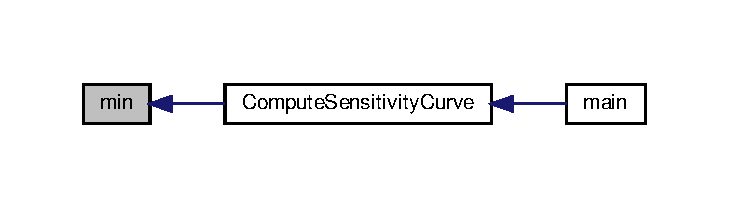
\includegraphics[width=350pt]{initialsimulation_8c_a2f8edc4561e9744ed4233b205fa7ec32_icgraph}
\end{center}
\end{figure}
\mbox{\Hypertarget{initialsimulation_8c_a435ef393d7d5394df67d5da81c108c7d}\label{initialsimulation_8c_a435ef393d7d5394df67d5da81c108c7d}} 
\index{initialsimulation.\+c@{initialsimulation.\+c}!square@{square}}
\index{square@{square}!initialsimulation.\+c@{initialsimulation.\+c}}
\subsubsection{\texorpdfstring{square()}{square()}}
{\footnotesize\ttfamily double square (\begin{DoxyParamCaption}\item[{double}]{x }\end{DoxyParamCaption})\hspace{0.3cm}{\ttfamily [inline]}}



Definition at line 84 of file initialsimulation.\+c.



References quickplot\+::x.



Referenced by chi\+D\+C\+Norm(), chi\+D\+C\+Spectral(), and likelihood().


\begin{DoxyCode}
85 \{
86   \textcolor{keywordflow}{return} \hyperlink{namespacequickplot_a81eab613e6132e2f34362e0d796374b6}{x}*\hyperlink{namespacequickplot_a81eab613e6132e2f34362e0d796374b6}{x};
87 \}
\end{DoxyCode}
Here is the caller graph for this function\+:
\nopagebreak
\begin{figure}[H]
\begin{center}
\leavevmode
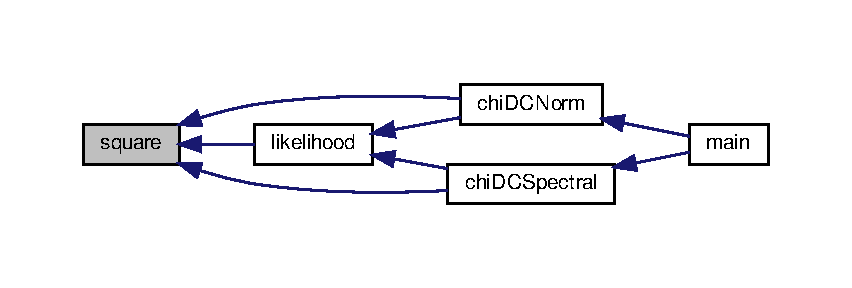
\includegraphics[width=350pt]{initialsimulation_8c_a435ef393d7d5394df67d5da81c108c7d_icgraph}
\end{center}
\end{figure}


\subsection{Variable Documentation}
\mbox{\Hypertarget{initialsimulation_8c_aa61745407a26c87961303a3c321dbba0}\label{initialsimulation_8c_aa61745407a26c87961303a3c321dbba0}} 
\index{initialsimulation.\+c@{initialsimulation.\+c}!chi2\+\_\+goal@{chi2\+\_\+goal}}
\index{chi2\+\_\+goal@{chi2\+\_\+goal}!initialsimulation.\+c@{initialsimulation.\+c}}
\subsubsection{\texorpdfstring{chi2\+\_\+goal}{chi2\_goal}}
{\footnotesize\ttfamily const double chi2\+\_\+goal = 2.\+7}



Definition at line 57 of file initialsimulation.\+c.



Referenced by Do\+Chi\+Square().

\mbox{\Hypertarget{initialsimulation_8c_a9d56cc3e601b27fad6831203a4626bd2}\label{initialsimulation_8c_a9d56cc3e601b27fad6831203a4626bd2}} 
\index{initialsimulation.\+c@{initialsimulation.\+c}!deltacp@{deltacp}}
\index{deltacp@{deltacp}!initialsimulation.\+c@{initialsimulation.\+c}}
\subsubsection{\texorpdfstring{deltacp}{deltacp}}
{\footnotesize\ttfamily double deltacp}



Definition at line 42 of file initialsimulation.\+c.



Referenced by Compute\+Sensitivity\+Curve(), and main().

\mbox{\Hypertarget{initialsimulation_8c_a76f2e70c9fc2a87ebcc598a0e021d2e6}\label{initialsimulation_8c_a76f2e70c9fc2a87ebcc598a0e021d2e6}} 
\index{initialsimulation.\+c@{initialsimulation.\+c}!gsl\+\_\+func@{gsl\+\_\+func}}
\index{gsl\+\_\+func@{gsl\+\_\+func}!initialsimulation.\+c@{initialsimulation.\+c}}
\subsubsection{\texorpdfstring{gsl\+\_\+func}{gsl\_func}}
{\footnotesize\ttfamily gsl\+\_\+function gsl\+\_\+func}



Definition at line 52 of file initialsimulation.\+c.



Referenced by Compute\+Sensitivity\+Curve(), and main().

\mbox{\Hypertarget{initialsimulation_8c_a4849c92a9edd1a0b4d2ff01484cebc91}\label{initialsimulation_8c_a4849c92a9edd1a0b4d2ff01484cebc91}} 
\index{initialsimulation.\+c@{initialsimulation.\+c}!input\+\_\+errors@{input\+\_\+errors}}
\index{input\+\_\+errors@{input\+\_\+errors}!initialsimulation.\+c@{initialsimulation.\+c}}
\subsubsection{\texorpdfstring{input\+\_\+errors}{input\_errors}}
{\footnotesize\ttfamily glb\+\_\+params input\+\_\+errors}



Definition at line 47 of file initialsimulation.\+c.



Referenced by Compute\+Sensitivity\+Curve(), and main().

\mbox{\Hypertarget{initialsimulation_8c_a3c9a8dabf1ad4dafa47e2d8002a71b44}\label{initialsimulation_8c_a3c9a8dabf1ad4dafa47e2d8002a71b44}} 
\index{initialsimulation.\+c@{initialsimulation.\+c}!ldm@{ldm}}
\index{ldm@{ldm}!initialsimulation.\+c@{initialsimulation.\+c}}
\subsubsection{\texorpdfstring{ldm}{ldm}}
{\footnotesize\ttfamily double ldm}



Definition at line 42 of file initialsimulation.\+c.



Referenced by Compute\+Sensitivity\+Curve(), and main().

\mbox{\Hypertarget{initialsimulation_8c_aa1edd4d864d9e90a1f10a7d13a68a885}\label{initialsimulation_8c_aa1edd4d864d9e90a1f10a7d13a68a885}} 
\index{initialsimulation.\+c@{initialsimulation.\+c}!logs22th13\+\_\+precision@{logs22th13\+\_\+precision}}
\index{logs22th13\+\_\+precision@{logs22th13\+\_\+precision}!initialsimulation.\+c@{initialsimulation.\+c}}
\subsubsection{\texorpdfstring{logs22th13\+\_\+precision}{logs22th13\_precision}}
{\footnotesize\ttfamily const double logs22th13\+\_\+precision = 0.\+005}



Definition at line 59 of file initialsimulation.\+c.



Referenced by Compute\+Sensitivity\+Curve().

\mbox{\Hypertarget{initialsimulation_8c_aa66d6bca132b398b255c2fd11ae6e7cc}\label{initialsimulation_8c_aa66d6bca132b398b255c2fd11ae6e7cc}} 
\index{initialsimulation.\+c@{initialsimulation.\+c}!max\+\_\+runtime@{max\+\_\+runtime}}
\index{max\+\_\+runtime@{max\+\_\+runtime}!initialsimulation.\+c@{initialsimulation.\+c}}
\subsubsection{\texorpdfstring{max\+\_\+runtime}{max\_runtime}}
{\footnotesize\ttfamily const double max\+\_\+runtime = 1e4}



Definition at line 56 of file initialsimulation.\+c.



Referenced by Compute\+Sensitivity\+Curve().

\mbox{\Hypertarget{initialsimulation_8c_a0a8e978504303b8dcd44cb9329b4cfc4}\label{initialsimulation_8c_a0a8e978504303b8dcd44cb9329b4cfc4}} 
\index{initialsimulation.\+c@{initialsimulation.\+c}!min\+\_\+runtime@{min\+\_\+runtime}}
\index{min\+\_\+runtime@{min\+\_\+runtime}!initialsimulation.\+c@{initialsimulation.\+c}}
\subsubsection{\texorpdfstring{min\+\_\+runtime}{min\_runtime}}
{\footnotesize\ttfamily const double min\+\_\+runtime = 1e-\/2}



Definition at line 55 of file initialsimulation.\+c.



Referenced by Compute\+Sensitivity\+Curve().

\mbox{\Hypertarget{initialsimulation_8c_a612d6b5b01674a0aec144bf224de6879}\label{initialsimulation_8c_a612d6b5b01674a0aec144bf224de6879}} 
\index{initialsimulation.\+c@{initialsimulation.\+c}!M\+Y\+F\+I\+L\+E1@{M\+Y\+F\+I\+L\+E1}}
\index{M\+Y\+F\+I\+L\+E1@{M\+Y\+F\+I\+L\+E1}!initialsimulation.\+c@{initialsimulation.\+c}}
\subsubsection{\texorpdfstring{M\+Y\+F\+I\+L\+E1}{MYFILE1}}
{\footnotesize\ttfamily char M\+Y\+F\+I\+L\+E1\mbox{[}$\,$\mbox{]} =\char`\"{}histsima.\+dat\char`\"{}}



Definition at line 34 of file initialsimulation.\+c.



Referenced by main().

\mbox{\Hypertarget{initialsimulation_8c_adfc2d3d253f6255b799065aa32d95cb2}\label{initialsimulation_8c_adfc2d3d253f6255b799065aa32d95cb2}} 
\index{initialsimulation.\+c@{initialsimulation.\+c}!M\+Y\+F\+I\+L\+E2@{M\+Y\+F\+I\+L\+E2}}
\index{M\+Y\+F\+I\+L\+E2@{M\+Y\+F\+I\+L\+E2}!initialsimulation.\+c@{initialsimulation.\+c}}
\subsubsection{\texorpdfstring{M\+Y\+F\+I\+L\+E2}{MYFILE2}}
{\footnotesize\ttfamily char M\+Y\+F\+I\+L\+E2\mbox{[}$\,$\mbox{]} =\char`\"{}histsimb.\+dat\char`\"{}}



Definition at line 35 of file initialsimulation.\+c.



Referenced by main().

\mbox{\Hypertarget{initialsimulation_8c_ac1dafa9fa032f3fd9126bad6b7a9850c}\label{initialsimulation_8c_ac1dafa9fa032f3fd9126bad6b7a9850c}} 
\index{initialsimulation.\+c@{initialsimulation.\+c}!M\+Y\+F\+I\+L\+E3@{M\+Y\+F\+I\+L\+E3}}
\index{M\+Y\+F\+I\+L\+E3@{M\+Y\+F\+I\+L\+E3}!initialsimulation.\+c@{initialsimulation.\+c}}
\subsubsection{\texorpdfstring{M\+Y\+F\+I\+L\+E3}{MYFILE3}}
{\footnotesize\ttfamily char M\+Y\+F\+I\+L\+E3\mbox{[}$\,$\mbox{]} =\char`\"{}histsim1.\+dat\char`\"{}}



Definition at line 36 of file initialsimulation.\+c.

\mbox{\Hypertarget{initialsimulation_8c_a9b42b07c83ecf6e931fc25d97a107cf0}\label{initialsimulation_8c_a9b42b07c83ecf6e931fc25d97a107cf0}} 
\index{initialsimulation.\+c@{initialsimulation.\+c}!s@{s}}
\index{s@{s}!initialsimulation.\+c@{initialsimulation.\+c}}
\subsubsection{\texorpdfstring{s}{s}}
{\footnotesize\ttfamily gsl\+\_\+root\+\_\+fsolver$\ast$ s}



Definition at line 51 of file initialsimulation.\+c.



Referenced by Compute\+Sensitivity\+Curve(), and main().

\mbox{\Hypertarget{initialsimulation_8c_a188db76c6a2dc2aa72024eb9cfb5eee2}\label{initialsimulation_8c_a188db76c6a2dc2aa72024eb9cfb5eee2}} 
\index{initialsimulation.\+c@{initialsimulation.\+c}!sdm@{sdm}}
\index{sdm@{sdm}!initialsimulation.\+c@{initialsimulation.\+c}}
\subsubsection{\texorpdfstring{sdm}{sdm}}
{\footnotesize\ttfamily double sdm}



Definition at line 42 of file initialsimulation.\+c.



Referenced by Compute\+Sensitivity\+Curve(), and main().

\mbox{\Hypertarget{initialsimulation_8c_af986a51f33f1570fd3fc8186dd81d866}\label{initialsimulation_8c_af986a51f33f1570fd3fc8186dd81d866}} 
\index{initialsimulation.\+c@{initialsimulation.\+c}!sigma\+\_\+binbin@{sigma\+\_\+binbin}}
\index{sigma\+\_\+binbin@{sigma\+\_\+binbin}!initialsimulation.\+c@{initialsimulation.\+c}}
\subsubsection{\texorpdfstring{sigma\+\_\+binbin}{sigma\_binbin}}
{\footnotesize\ttfamily double sigma\+\_\+binbin = 0.\+0}



Definition at line 64 of file initialsimulation.\+c.



Referenced by chi\+D\+C\+Spectral().

\mbox{\Hypertarget{initialsimulation_8c_ac40fbcecee7fb042256f95763d5c1c68}\label{initialsimulation_8c_ac40fbcecee7fb042256f95763d5c1c68}} 
\index{initialsimulation.\+c@{initialsimulation.\+c}!sys\+\_\+errors@{sys\+\_\+errors}}
\index{sys\+\_\+errors@{sys\+\_\+errors}!initialsimulation.\+c@{initialsimulation.\+c}}
\subsubsection{\texorpdfstring{sys\+\_\+errors}{sys\_errors}}
{\footnotesize\ttfamily double sys\+\_\+errors\mbox{[}\hyperlink{initialsimulation_8c_aa985f5d78fe22e2bf9115004a82d9008}{M\+A\+X\+\_\+\+S\+YS}\mbox{]}}



Definition at line 62 of file initialsimulation.\+c.

\mbox{\Hypertarget{initialsimulation_8c_a6ce721d0fe57253b204857c23ed0e4db}\label{initialsimulation_8c_a6ce721d0fe57253b204857c23ed0e4db}} 
\index{initialsimulation.\+c@{initialsimulation.\+c}!sys\+\_\+startval@{sys\+\_\+startval}}
\index{sys\+\_\+startval@{sys\+\_\+startval}!initialsimulation.\+c@{initialsimulation.\+c}}
\subsubsection{\texorpdfstring{sys\+\_\+startval}{sys\_startval}}
{\footnotesize\ttfamily double sys\+\_\+startval\mbox{[}\hyperlink{initialsimulation_8c_aa985f5d78fe22e2bf9115004a82d9008}{M\+A\+X\+\_\+\+S\+YS}\mbox{]}}



Definition at line 63 of file initialsimulation.\+c.



Referenced by chi\+D\+C\+Norm(), chi\+D\+C\+Spectral(), Do\+Chi\+Square(), and main().

\mbox{\Hypertarget{initialsimulation_8c_a00bb11e935f05b5bb392ec7cc02a1478}\label{initialsimulation_8c_a00bb11e935f05b5bb392ec7cc02a1478}} 
\index{initialsimulation.\+c@{initialsimulation.\+c}!T@{T}}
\index{T@{T}!initialsimulation.\+c@{initialsimulation.\+c}}
\subsubsection{\texorpdfstring{T}{T}}
{\footnotesize\ttfamily const gsl\+\_\+root\+\_\+fsolver\+\_\+type$\ast$ T}



Definition at line 50 of file initialsimulation.\+c.



Referenced by main().

\mbox{\Hypertarget{initialsimulation_8c_a7b09cafa395dbf045d36fc6dad50319a}\label{initialsimulation_8c_a7b09cafa395dbf045d36fc6dad50319a}} 
\index{initialsimulation.\+c@{initialsimulation.\+c}!test\+\_\+values@{test\+\_\+values}}
\index{test\+\_\+values@{test\+\_\+values}!initialsimulation.\+c@{initialsimulation.\+c}}
\subsubsection{\texorpdfstring{test\+\_\+values}{test\_values}}
{\footnotesize\ttfamily glb\+\_\+params test\+\_\+values}



Definition at line 46 of file initialsimulation.\+c.



Referenced by Compute\+Sensitivity\+Curve(), Do\+Chi\+Square(), and main().

\mbox{\Hypertarget{initialsimulation_8c_a34595bc67066b681fdf55138851f5537}\label{initialsimulation_8c_a34595bc67066b681fdf55138851f5537}} 
\index{initialsimulation.\+c@{initialsimulation.\+c}!theta12@{theta12}}
\index{theta12@{theta12}!initialsimulation.\+c@{initialsimulation.\+c}}
\subsubsection{\texorpdfstring{theta12}{theta12}}
{\footnotesize\ttfamily double theta12}



Definition at line 42 of file initialsimulation.\+c.



Referenced by Compute\+Sensitivity\+Curve(), and main().

\mbox{\Hypertarget{initialsimulation_8c_a16d90a56a2e53f1e0ce749a1924f5e91}\label{initialsimulation_8c_a16d90a56a2e53f1e0ce749a1924f5e91}} 
\index{initialsimulation.\+c@{initialsimulation.\+c}!theta13@{theta13}}
\index{theta13@{theta13}!initialsimulation.\+c@{initialsimulation.\+c}}
\subsubsection{\texorpdfstring{theta13}{theta13}}
{\footnotesize\ttfamily double theta13}



Definition at line 42 of file initialsimulation.\+c.



Referenced by Compute\+Sensitivity\+Curve(), and main().

\mbox{\Hypertarget{initialsimulation_8c_ad7eb34b77c1ced121f217184784ca4ca}\label{initialsimulation_8c_ad7eb34b77c1ced121f217184784ca4ca}} 
\index{initialsimulation.\+c@{initialsimulation.\+c}!theta23@{theta23}}
\index{theta23@{theta23}!initialsimulation.\+c@{initialsimulation.\+c}}
\subsubsection{\texorpdfstring{theta23}{theta23}}
{\footnotesize\ttfamily double theta23}



Definition at line 42 of file initialsimulation.\+c.



Referenced by Compute\+Sensitivity\+Curve(), and main().

\mbox{\Hypertarget{initialsimulation_8c_a04b2e1a70c7d99ae440fc0b97b42bb2b}\label{initialsimulation_8c_a04b2e1a70c7d99ae440fc0b97b42bb2b}} 
\index{initialsimulation.\+c@{initialsimulation.\+c}!true\+\_\+values@{true\+\_\+values}}
\index{true\+\_\+values@{true\+\_\+values}!initialsimulation.\+c@{initialsimulation.\+c}}
\subsubsection{\texorpdfstring{true\+\_\+values}{true\_values}}
{\footnotesize\ttfamily glb\+\_\+params true\+\_\+values}



Definition at line 45 of file initialsimulation.\+c.



Referenced by Compute\+Sensitivity\+Curve(), and main().

\mbox{\Hypertarget{initialsimulation_8c_a8ceb9a82655d4344fa7db3b8d0dc8afb}\label{initialsimulation_8c_a8ceb9a82655d4344fa7db3b8d0dc8afb}} 
\index{initialsimulation.\+c@{initialsimulation.\+c}!t\+Steps@{t\+Steps}}
\index{t\+Steps@{t\+Steps}!initialsimulation.\+c@{initialsimulation.\+c}}
\subsubsection{\texorpdfstring{t\+Steps}{tSteps}}
{\footnotesize\ttfamily const int t\+Steps = 30}



Definition at line 58 of file initialsimulation.\+c.



Referenced by Compute\+Sensitivity\+Curve().


\hypertarget{initialsimulation_8h}{}\section{initialsimulation.\+h File Reference}
\label{initialsimulation_8h}\index{initialsimulation.\+h@{initialsimulation.\+h}}
{\ttfamily \#include $<$stdio.\+h$>$}\newline
{\ttfamily \#include $<$stdlib.\+h$>$}\newline
{\ttfamily \#include $<$math.\+h$>$}\newline
{\ttfamily \#include $<$string.\+h$>$}\newline
{\ttfamily \#include $<$gsl/gsl\+\_\+math.\+h$>$}\newline
{\ttfamily \#include $<$gsl/gsl\+\_\+roots.\+h$>$}\newline
{\ttfamily \#include $<$gsl/gsl\+\_\+errno.\+h$>$}\newline
{\ttfamily \#include $<$globes/globes.\+h$>$}\newline
{\ttfamily \#include \char`\"{}myio.\+h\char`\"{}}\newline
Include dependency graph for initialsimulation.\+h\+:
\nopagebreak
\begin{figure}[H]
\begin{center}
\leavevmode
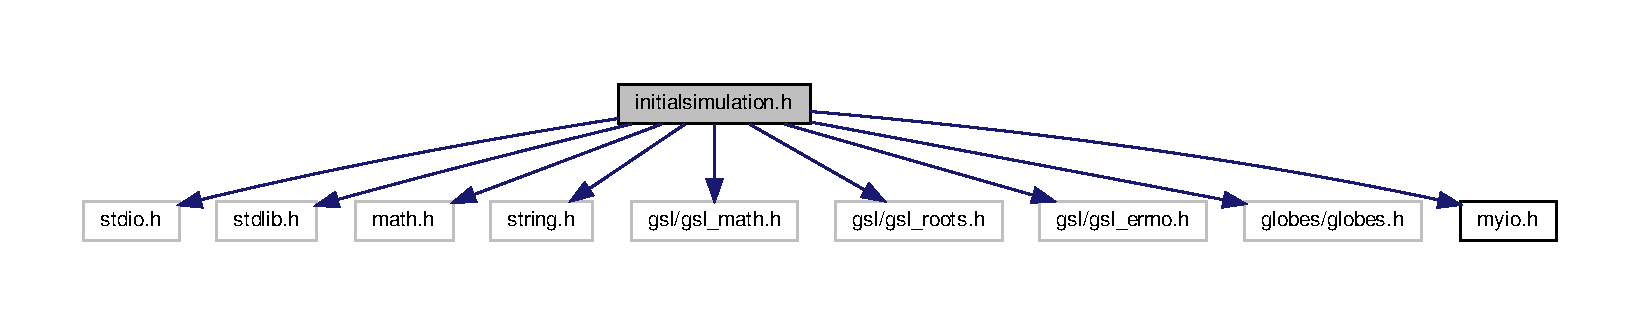
\includegraphics[width=350pt]{initialsimulation_8h__incl}
\end{center}
\end{figure}
This graph shows which files directly or indirectly include this file\+:
\nopagebreak
\begin{figure}[H]
\begin{center}
\leavevmode
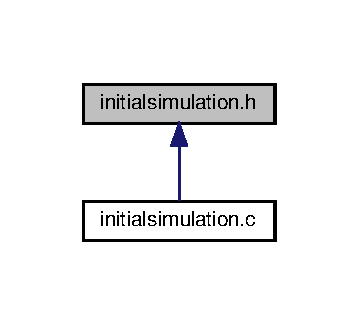
\includegraphics[width=172pt]{initialsimulation_8h__dep__incl}
\end{center}
\end{figure}

\hypertarget{myio_8c}{}\section{myio.\+c File Reference}
\label{myio_8c}\index{myio.\+c@{myio.\+c}}
{\ttfamily \#include \char`\"{}myio.\+h\char`\"{}}\newline
{\ttfamily \#include $<$stdio.\+h$>$}\newline
{\ttfamily \#include $<$string.\+h$>$}\newline
Include dependency graph for myio.\+c\+:\nopagebreak
\begin{figure}[H]
\begin{center}
\leavevmode
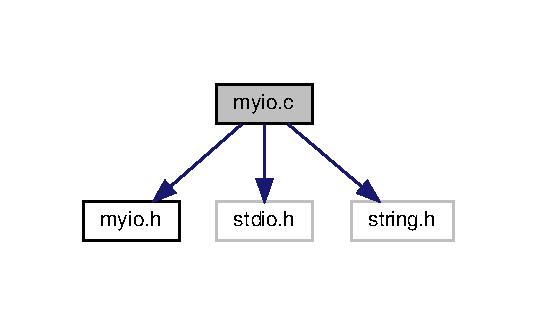
\includegraphics[width=258pt]{myio_8c__incl}
\end{center}
\end{figure}
\subsection*{Functions}
\begin{DoxyCompactItemize}
\item 
void \hyperlink{myio_8c_ad28713ee02cd79dc48ad1ee2a7b62177}{Init\+Output} (char $\ast$filename, char $\ast$headline)
\item 
void \hyperlink{myio_8c_a689d604a981e54de08599dc9cb597579}{Add\+To\+Output} (double n1, double n2, double n3)
\item 
void \hyperlink{myio_8c_ae9af054c63cf3b736da1ee7151f69d2c}{Add\+To\+Output2} (double n1, double n2)
\end{DoxyCompactItemize}
\subsection*{Variables}
\begin{DoxyCompactItemize}
\item 
static char $\ast$ \hyperlink{myio_8c_a0000f7a2b68b443a53bc17affd3770ce}{T\+H\+E\+F\+I\+LE}
\end{DoxyCompactItemize}


\subsection{Function Documentation}
\mbox{\Hypertarget{myio_8c_a689d604a981e54de08599dc9cb597579}\label{myio_8c_a689d604a981e54de08599dc9cb597579}} 
\index{myio.\+c@{myio.\+c}!Add\+To\+Output@{Add\+To\+Output}}
\index{Add\+To\+Output@{Add\+To\+Output}!myio.\+c@{myio.\+c}}
\subsubsection{\texorpdfstring{Add\+To\+Output()}{AddToOutput()}}
{\footnotesize\ttfamily void Add\+To\+Output (\begin{DoxyParamCaption}\item[{double}]{n1,  }\item[{double}]{n2,  }\item[{double}]{n3 }\end{DoxyParamCaption})}

\mbox{\Hypertarget{myio_8c_ae9af054c63cf3b736da1ee7151f69d2c}\label{myio_8c_ae9af054c63cf3b736da1ee7151f69d2c}} 
\index{myio.\+c@{myio.\+c}!Add\+To\+Output2@{Add\+To\+Output2}}
\index{Add\+To\+Output2@{Add\+To\+Output2}!myio.\+c@{myio.\+c}}
\subsubsection{\texorpdfstring{Add\+To\+Output2()}{AddToOutput2()}}
{\footnotesize\ttfamily void Add\+To\+Output2 (\begin{DoxyParamCaption}\item[{double}]{n1,  }\item[{double}]{n2 }\end{DoxyParamCaption})}

Here is the caller graph for this function\+:\nopagebreak
\begin{figure}[H]
\begin{center}
\leavevmode
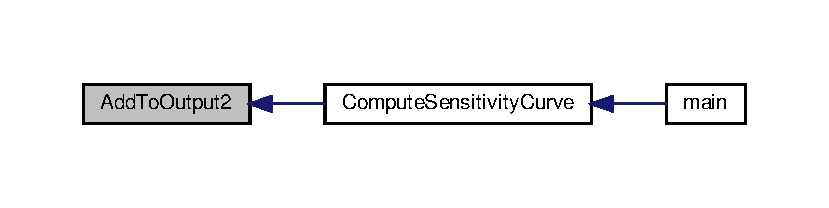
\includegraphics[width=350pt]{myio_8c_ae9af054c63cf3b736da1ee7151f69d2c_icgraph}
\end{center}
\end{figure}
\mbox{\Hypertarget{myio_8c_ad28713ee02cd79dc48ad1ee2a7b62177}\label{myio_8c_ad28713ee02cd79dc48ad1ee2a7b62177}} 
\index{myio.\+c@{myio.\+c}!Init\+Output@{Init\+Output}}
\index{Init\+Output@{Init\+Output}!myio.\+c@{myio.\+c}}
\subsubsection{\texorpdfstring{Init\+Output()}{InitOutput()}}
{\footnotesize\ttfamily void Init\+Output (\begin{DoxyParamCaption}\item[{char $\ast$}]{filename,  }\item[{char $\ast$}]{headline }\end{DoxyParamCaption})}

Here is the caller graph for this function\+:\nopagebreak
\begin{figure}[H]
\begin{center}
\leavevmode
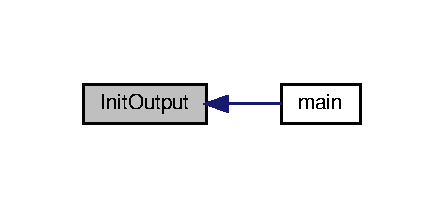
\includegraphics[width=213pt]{myio_8c_ad28713ee02cd79dc48ad1ee2a7b62177_icgraph}
\end{center}
\end{figure}


\subsection{Variable Documentation}
\mbox{\Hypertarget{myio_8c_a0000f7a2b68b443a53bc17affd3770ce}\label{myio_8c_a0000f7a2b68b443a53bc17affd3770ce}} 
\index{myio.\+c@{myio.\+c}!T\+H\+E\+F\+I\+LE@{T\+H\+E\+F\+I\+LE}}
\index{T\+H\+E\+F\+I\+LE@{T\+H\+E\+F\+I\+LE}!myio.\+c@{myio.\+c}}
\subsubsection{\texorpdfstring{T\+H\+E\+F\+I\+LE}{THEFILE}}
{\footnotesize\ttfamily char$\ast$ T\+H\+E\+F\+I\+LE\hspace{0.3cm}{\ttfamily [static]}}


\hypertarget{myio_8h}{}\section{myio.\+h File Reference}
\label{myio_8h}\index{myio.\+h@{myio.\+h}}
This graph shows which files directly or indirectly include this file\+:\nopagebreak
\begin{figure}[H]
\begin{center}
\leavevmode
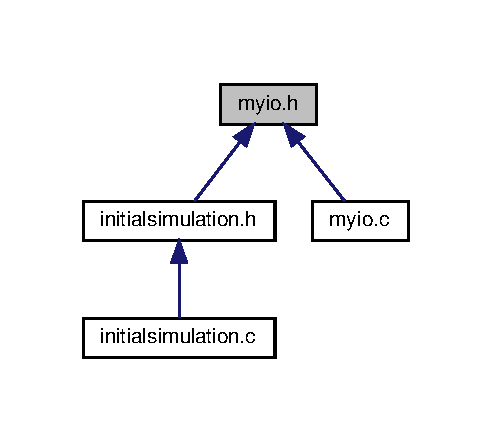
\includegraphics[width=236pt]{myio_8h__dep__incl}
\end{center}
\end{figure}
\subsection*{Functions}
\begin{DoxyCompactItemize}
\item 
void \hyperlink{myio_8h_ad28713ee02cd79dc48ad1ee2a7b62177}{Init\+Output} (char $\ast$filename, char $\ast$headline)
\item 
void \hyperlink{myio_8h_a689d604a981e54de08599dc9cb597579}{Add\+To\+Output} (double n1, double n2, double n3)
\item 
void \hyperlink{myio_8h_ae9af054c63cf3b736da1ee7151f69d2c}{Add\+To\+Output2} (double n1, double n2)
\end{DoxyCompactItemize}


\subsection{Function Documentation}
\mbox{\Hypertarget{myio_8h_a689d604a981e54de08599dc9cb597579}\label{myio_8h_a689d604a981e54de08599dc9cb597579}} 
\index{myio.\+h@{myio.\+h}!Add\+To\+Output@{Add\+To\+Output}}
\index{Add\+To\+Output@{Add\+To\+Output}!myio.\+h@{myio.\+h}}
\subsubsection{\texorpdfstring{Add\+To\+Output()}{AddToOutput()}}
{\footnotesize\ttfamily void Add\+To\+Output (\begin{DoxyParamCaption}\item[{double}]{n1,  }\item[{double}]{n2,  }\item[{double}]{n3 }\end{DoxyParamCaption})}



Definition at line 48 of file myio.\+c.



References T\+H\+E\+F\+I\+LE.


\begin{DoxyCode}
49 \{
50  \textcolor{keywordflow}{if}(strlen(\hyperlink{myio_8c_a0000f7a2b68b443a53bc17affd3770ce}{THEFILE})==0) printf(\textcolor{stringliteral}{"%g %g %f \(\backslash\)n"},n1,n2,n3);
51  \textcolor{keywordflow}{else} 
52  \{
53    FILE* f=fopen(\hyperlink{myio_8c_a0000f7a2b68b443a53bc17affd3770ce}{THEFILE}, \textcolor{stringliteral}{"a"});
54    \textcolor{keywordflow}{if} (!f)
55    \{
56      printf(\textcolor{stringliteral}{"File cannot be opened!\(\backslash\)n"});
57      \hyperlink{myio_8c_a0000f7a2b68b443a53bc17affd3770ce}{THEFILE}[0]=0;
58    \}
59    \textcolor{keywordflow}{else}
60    \{
61     fprintf(f,\textcolor{stringliteral}{"%g %g %f \(\backslash\)n"},n1,n2,n3);
62     fclose(f);
63    \}
64  \}
65 \}
\end{DoxyCode}
\mbox{\Hypertarget{myio_8h_ae9af054c63cf3b736da1ee7151f69d2c}\label{myio_8h_ae9af054c63cf3b736da1ee7151f69d2c}} 
\index{myio.\+h@{myio.\+h}!Add\+To\+Output2@{Add\+To\+Output2}}
\index{Add\+To\+Output2@{Add\+To\+Output2}!myio.\+h@{myio.\+h}}
\subsubsection{\texorpdfstring{Add\+To\+Output2()}{AddToOutput2()}}
{\footnotesize\ttfamily void Add\+To\+Output2 (\begin{DoxyParamCaption}\item[{double}]{n1,  }\item[{double}]{n2 }\end{DoxyParamCaption})}



Definition at line 67 of file myio.\+c.



References T\+H\+E\+F\+I\+LE.



Referenced by Compute\+Sensitivity\+Curve().


\begin{DoxyCode}
68 \{
69  \textcolor{keywordflow}{if}(strlen(\hyperlink{myio_8c_a0000f7a2b68b443a53bc17affd3770ce}{THEFILE})==0) printf(\textcolor{stringliteral}{"%g %g \(\backslash\)n"},n1,n2);
70  \textcolor{keywordflow}{else} 
71  \{
72    FILE* f=fopen(\hyperlink{myio_8c_a0000f7a2b68b443a53bc17affd3770ce}{THEFILE}, \textcolor{stringliteral}{"a"});
73    \textcolor{keywordflow}{if} (!f)
74    \{
75      printf(\textcolor{stringliteral}{"File cannot be opened!\(\backslash\)n"});
76      \hyperlink{myio_8c_a0000f7a2b68b443a53bc17affd3770ce}{THEFILE}[0]=0;
77    \}
78    \textcolor{keywordflow}{else}
79    \{
80     fprintf(f,\textcolor{stringliteral}{"%g %g \(\backslash\)n"},n1,n2);
81     fclose(f);
82    \}
83  \}
84 \}
\end{DoxyCode}
Here is the caller graph for this function\+:\nopagebreak
\begin{figure}[H]
\begin{center}
\leavevmode
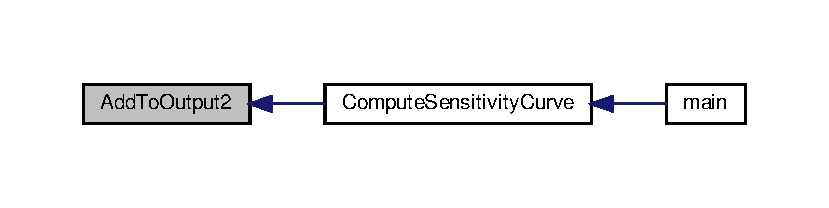
\includegraphics[width=350pt]{myio_8h_ae9af054c63cf3b736da1ee7151f69d2c_icgraph}
\end{center}
\end{figure}
\mbox{\Hypertarget{myio_8h_ad28713ee02cd79dc48ad1ee2a7b62177}\label{myio_8h_ad28713ee02cd79dc48ad1ee2a7b62177}} 
\index{myio.\+h@{myio.\+h}!Init\+Output@{Init\+Output}}
\index{Init\+Output@{Init\+Output}!myio.\+h@{myio.\+h}}
\subsubsection{\texorpdfstring{Init\+Output()}{InitOutput()}}
{\footnotesize\ttfamily void Init\+Output (\begin{DoxyParamCaption}\item[{char $\ast$}]{filename,  }\item[{char $\ast$}]{headline }\end{DoxyParamCaption})}



Definition at line 29 of file myio.\+c.



References T\+H\+E\+F\+I\+LE.



Referenced by main().


\begin{DoxyCode}
30 \{
31  \hyperlink{myio_8c_a0000f7a2b68b443a53bc17affd3770ce}{THEFILE}=filename;
32  \textcolor{keywordflow}{if}(strlen(\hyperlink{myio_8c_a0000f7a2b68b443a53bc17affd3770ce}{THEFILE})==0) printf(headline);
33  \textcolor{keywordflow}{else} 
34  \{
35    FILE* f=fopen(\hyperlink{myio_8c_a0000f7a2b68b443a53bc17affd3770ce}{THEFILE}, \textcolor{stringliteral}{"w"});
36    \textcolor{keywordflow}{if} (!f)
37    \{
38      printf(\textcolor{stringliteral}{"File cannot be opened!\(\backslash\)n"});
39      \hyperlink{myio_8c_a0000f7a2b68b443a53bc17affd3770ce}{THEFILE}[0]=0;
40    \}
41    \textcolor{keywordflow}{else} \{
42     fprintf(f,headline);
43     fclose(f);
44    \}
45  \}
46 \}
\end{DoxyCode}
Here is the caller graph for this function\+:\nopagebreak
\begin{figure}[H]
\begin{center}
\leavevmode
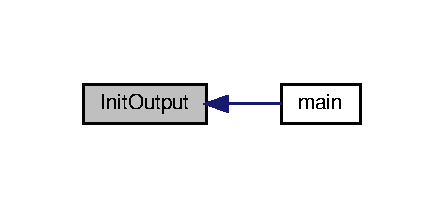
\includegraphics[width=213pt]{myio_8h_ad28713ee02cd79dc48ad1ee2a7b62177_icgraph}
\end{center}
\end{figure}

\hypertarget{quickplot_8py}{}\section{Plotting/quickplot.py File Reference}
\label{quickplot_8py}\index{Plotting/quickplot.\+py@{Plotting/quickplot.\+py}}
\subsection*{Namespaces}
\begin{DoxyCompactItemize}
\item 
 \hyperlink{namespacequickplot}{quickplot}
\end{DoxyCompactItemize}
\subsection*{Variables}
\begin{DoxyCompactItemize}
\item 
\hyperlink{namespacequickplot_a81eab613e6132e2f34362e0d796374b6}{quickplot.\+x}
\item 
\hyperlink{namespacequickplot_a010fcab3235443a7866d032bea36b2e8}{quickplot.\+y}
\item 
\hyperlink{namespacequickplot_a26e9d46e54bdec05e3fe95d1105f5c63}{quickplot.\+unpack}
\item 
\hyperlink{namespacequickplot_a665c218bc9c59ff692bf90bfbf077344}{quickplot.\+weights}
\end{DoxyCompactItemize}

%--- End generated contents ---

% Index
\backmatter
\newpage
\phantomsection
\clearemptydoublepage
\addcontentsline{toc}{chapter}{Index}
\printindex

\end{document}
